\documentclass{article}
\usepackage{graphicx, amsmath, amssymb, hyperref, subcaption, cleveref, listings, float}

\usepackage[bottom]{footmisc}
\usepackage[margin=.70in]{geometry}
\title{Sistemi embedded}

\author{Giuseppe Capasso}
\renewcommand{\contentsname}{Indice}
\renewcommand{\refname}{Riferimenti}
\renewcommand{\figurename}{Figura}
\renewcommand{\tablename}{Tabella}

\crefformat{section}{\S#2#1#3}
\crefformat{subsection}{\S#2#1#3}
\crefformat{subsubsection}{\S#2#1#3}
\crefformat{figure}{#2Figura~#1#3}
\crefformat{footnote}{#2\footnotemark[#1]#3}
\crefformat{table}{#2Tabella~#1#3}

\crefname{lstlisting}{listato}{listati}
\Crefname{lstlisting}{Listato}{Listati}

\begin{document}

\pagestyle{plain}
\pagenumbering{roman}
\setcounter{page}{1}
\maketitle

\tableofcontents
\newpage

\pagenumbering{arabic}
\setcounter{page}{1}
\section{Architettura ARM}
\textbf{A}dvanced \textbf{R}isc \textbf{M}achine (ARM) è un progetto per realizzare un processore RISC con un modello basato su \textbf{I}ntellectual \textbf{P}roperty (IP): le aziende che scelgono di implementare ARM devono acquisire i progetti e poi occuparsi di mettere su silicio integrandosi con periferiche e e sistemi esterni producendo un \textbf{S}ystem \textbf{o}n \textbf{C}hip.

\subsection{Famiglie di processori ARM}
I processori ARM possono essere caratterizzati in $3$ grandi famiglie (profili) in base all'utilizzo principale dette \textbf{Cortex}:
\begin{itemize}
  \item Cortex M: profilo utilizzato per i micro-processori. Sistemi che si occupano di eseguire poche operazioni in ambito industriale;
  \item Cortex A: detto anche \textbf{application processor} per applicazioni ad alte performance con supporto alla virtualizzazione e sicurezza;
  \item Cortex R: processori adatti per le applicazioni di tipo real-time il cui focus è sulla \textit{safety} e sulla predicibilità delle operazioni e per questo più semplici;
\end{itemize}

Queste famiglie sono contraddistinte secondo la versione dell'architettura in cui vengono calate. Come mostrato in \cref{fig:arm-evolution}.

\begin{figure}[h]
  \begin{center}
    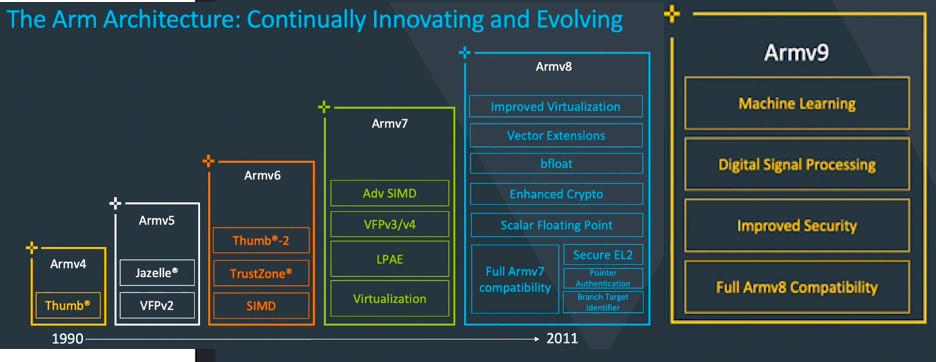
\includegraphics[width=0.95\textwidth]{./figures/ch1/arm-vision-architecture-roadmap.jpg}
  \end{center}
  \caption{Evoluzione dell'architettura ARM}\label{fig:arm-evolution}
\end{figure}

In ARMv6, sono state introdotte le prime istruzioni vettoriali (SIMD), TrustZone (per la sicurezza delle applicazioni) e l'ISA \textbf{Thumb2}. Thumb2 introduce istruzioni a lunghezza variabile a $16-bit$ a differenza di quelle a lunghezza fissa presenti in \textbf{Thumb} a partire da ARMv4. Per la struttura di Thumb e Thumb2 non è possibile avere la modalità di indirizzamento assoluto, ma è possibile specificare locazioni di memoria come \textit{offset} rispetto al PC. Questo rende il codice scritto per ARM \textbf{rilocabile} per costruzione.

Fino ad ARMv7, i processori sono a $32-bit$. A partire da \textbf{ARMv8}, l'architettura diventa a $64-bit$ (possibilità di retro-compatibilità a $32-bit$) introducendo supporto hardware alla virtualizzazione. 

\subsection{Cortex M}
Di seguito si fa riferimento alle architetture $M3$ e $M4$ perchè simili tra loro se non per qualche piccola differenza. Ad esempio, $M4$ ha un componente esplicito per il calcolo a virgola mobile (FPU). In \cref{fig:cortex-m4-arch}, è mostrato lo schema di riferimento utilizzato.

\begin{figure}[h]
  \begin{center}
    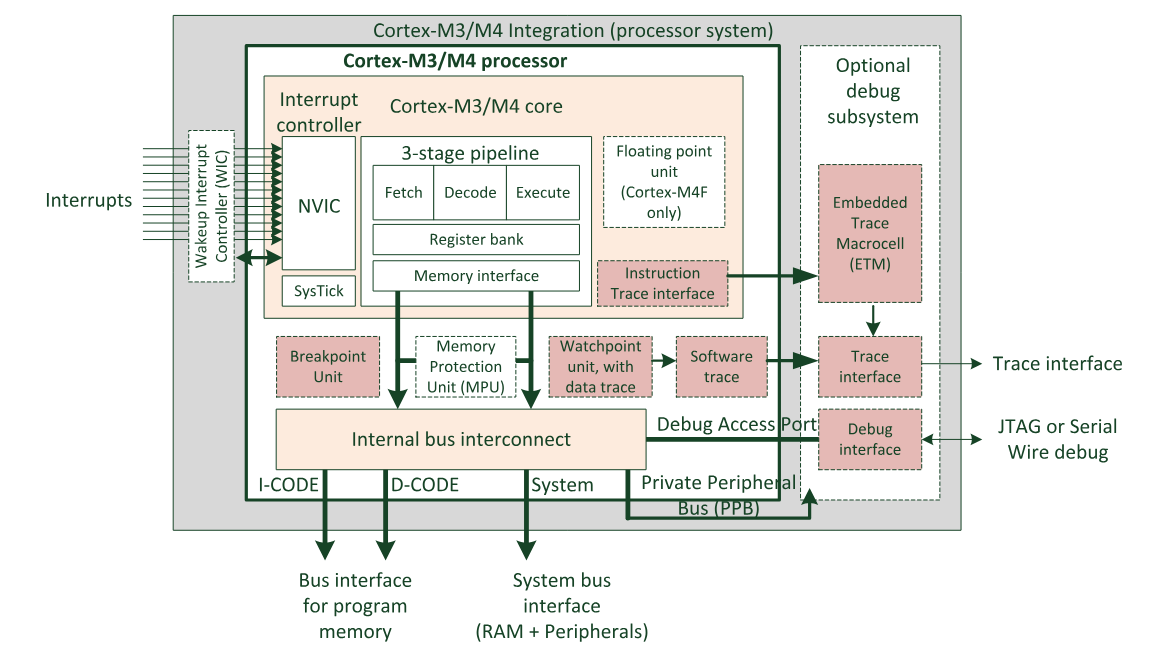
\includegraphics[width=0.95\textwidth]{./figures/ch1/cortex-m/arch.png}
  \end{center}
  \caption{Schema a blocchi di riferimento del Cortex-M3/M4}\label{fig:cortex-m4-arch}
\end{figure}

\paragraph{Cortex M4: FPU} Il Cortex-M4 include una unità dedicata al calcolo a virgola mobile. Questa unità ha un \textit{register file} dedicato da $32$ ($S0-S31$) registri a $32-bit$ (per operare a singola precisione). Questi possono essere visti (con l'\textbf{\textit{aliasing}}) anche come $16$ ($D0-D15$) registri a $64-bit$ (per operare a doppia precisione). Inoltre, sono presenti anche registri di controllo per le ordinarie operazioni in floating-point. Bisogna chiedersi fino a che livello c'è il supporto alle operazioni in virgola mobile poichè lo standard \textbf{\textit{IEEE-754}} richiede molte funzionalità come il supporto alle operazioni con numeri de-normalizzati, operazioni di \textbf{rounding} ecc. Data la mole di operazioni, la FPU consuma molta energia e spesso viene spenta quando non richiesta.

\paragraph{Assembler}
ARM prevede \textbf{\textit{UAL}} (unified assembler language) che aggiunge pseudo istruzioni per fare le operazioni più complicate o per complicare codice sia per Thumb che per Thumb2. UAL prevede pseudo-operazioni che richiedono più istruzioni. Ad esempio, l'assegnazione di una costante a $32-bit$ non è possibile a $16-bit$. UAL prevede un costrutto in cui l'assemblatore dedica un'area di memoria detta \textbf{\textit{LITERAL POOL}} in cui conserva le costanti a $32-bit$ con una $MOVE$.

\paragraph{Arm Architecture Procedure Call Standard: AAPCS}
ARM ha creato uno standard per far interagire programmi in C e assembler in cui viene standardizzato il modo in cui si scrivono le funzioni che richiamano il codice assembler (calling convention). Quando la funzione C passa fino a 4 parametri (a $32-bit$) per default il passaggio dei parametri avviene attraverso i primi 4 registri del processore ($R0 - R3$) e in $R0$ si scrive il risultato. Questa cosa serve quando il processore utilizza istruzioni non compliant con lo standard ieee-754 fp perchè il compilatore non usa cose nonstandard.

\paragraph{Stato di funzionamento e livelli di privilegio}
Il Cortex-M ha $3$ livelli di privilegio, presentati in \cref{fig:cortex-m-state}:

\begin{itemize}
  \item \textbf{handler mode}: utilizzato quando ci si trova a gestire un'eccezione o un'interruzione;
  \item \textbf{thread mode}: in questo stato viene eseguito il codice applicativo. Questa modalità è ulteriormente diviso in \textbf{\textit{thread mode privileged}} e \textbf{\textit{thread mode unpriviledge}}. La modalità di privilegio può essere gestita con il registro CONTROL;
\end{itemize}

\begin{figure}[h]
  \begin{center}
    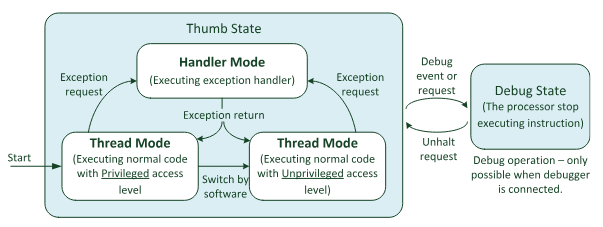
\includegraphics[width=0.95\textwidth]{./figures/ch1/cortex-m/state.png}
  \end{center}
  \caption{Stato e livelli di privilegio del cortex-M}\label{fig:cortex-m-state}
\end{figure}

Se si esegue codice \textbf{Bare metal}, tutto il codice applicativo è privilegiato; mentre se si esegue un sistema operativo, il codice privilegiato è quello riservato alle operazioni quali system-call, scheduler ecc.

Lo stato in cui si trova il processore è un concetto ortoganale a quello delle modalità ed è riferito alla tipologia di istruzioni che sta eseguendo. Nel cortex-M, il processore è sempre in \textbf{Thumb mode}, ma in Cortex-R o Cortex-A questo può essere anche in \textbf{ARM mode}. Inoltre, il processore può essere in \textbf{Debug State}.


\subsubsection{Core}
In \cref{fig:cortex-m4-arch}, la parte in giallo è detta \textbf{core}. È composta da una pipeline a $3$ stadi e un \textbf{\textit{register file}} composto da $16$ registri a $32-bit$: $R0-R15$. Tra questi, si distinguono:
\begin{itemize}
  \item $R15$: program counter (\textbf{PC});
  \item $R14$: link register (\textbf{LR}). Serve a rendere più efficiente la chiamata a funzione evitando di il PC nello stack.
  \item $R13$: stack pointer (\textbf{SP}). È un registro \textbf{banked}: a questo registro "logico" possono corrispondere diverse strutture fisiche dipendentemente dallo stato in cui ci si trova. Ad esempio, nel \textbf{\textit{68k}}, si trova $A7$ e $A7'$. In ARM, sono detti $PSP$ (\textbf{\textit{Process Stack Pointer}}) e $MSP$ (\textbf{\textit{Main Stack Pointer}})  
\end{itemize}

All'interno del core, c'è un'interfacciamento verso la memoria e la parte per la gestione delle interruzioni. In riferimento a quest'ultima, c'è l'NVIC (controller delle interruzioni) a cui è collegato il \textbf{SysTick} (contatore a $24-bit$ programmabile per avere interruzioni ogni $10ms$) che serve a scandire il tempo nel sistema attraverso delle interruzioni in relazione al clock fisico.

\paragraph{Registri speciali}
Oltre ai general purpose register ce ne sono alcuni particolari. Ad esempio, si è già parlato del registro \textit{CONTROL} che ha un bit detto \textit{SPSEL} per selezionare quale stack pointer utilizzare o il bit \textit{nPriv} per impostare la modalità di privilegio. Un altro bit importante è \textit{FPCA} che abilita il salvataggio dello stato della FPU che può essere critico poichè molto oneroso, ma parte di un eventuale contesto di un processo. In situazione di errore, non è necessario salvare magari perchè ci si trova in una situazione non recuperabile.

Un registro particolare è il \textit{FAULTMASK} che serve a mascherare le interruzioni (oltre a quelle hardware) via software per effettuare debug.

Il registro \textit{PRIMASK} è utile per disabilitare le interruzioni per le normali operazioni. Ad esempio, se si sta facendo un'operazione atomica si alza questo bit.

Infine, il registro \textit{BASEPRI} agisce sulle interruzione delle periferiche che possono essere disabilitate da un livello minimo in poi.

Lo \textit{Status} register contiene tutte le informazioni generiche per l'utente come il valore dei classici bit $N, Z, V, C, Q$. Per il bit $Q$ potrebbe essere fatto un discorso a parte sull'aritmetica a saturazione molto utilizzata nei sistemi DSP: Invece di saltare da una parte all'altra dell'intervallo di rappresentazione, si preferisce saturare all'estremo più vicino. Inoltre, è impensabile di controllare l'overflow ad ogni operazione con eventuale salto. In questo senso, il bit $Q$ è \textbf{\textit{sticky}} (deve essere resettato manualmente) e indica che c'è stata un'operazione.
Inoltre, in relazione al Cortex-M4, c'è il bit \textit{GE} (Greater Equal) che vengono utilizzati anche dalle opzioni SIMD. Per questo motivo ci sono $4$ flag \textit{GE} poichè il confronto può essere fatto su altrettanti coppie di valori. 
Infine, il registro di stato ha delle istruzioni apposite per impostare e salvare il suo valore:
\begin{itemize}
  \item MRS: move from register to status;
  \item MSR: move from status to register;
\end{itemize}

\paragraph{Eccezioni ed interruzioni}
Il core contiene il \textit{Nested Interrupt Vectored Controller} (\textbf{NVIC}) per gestire le interruzioni ed eccezioni. Alle eccezioni (\cref{fig:cortex-m-exception}) sono associate delle priorità: quella col numero più basso ha priorità maggiore. Le prime eccezioni sono quelle di sistema: da $0$ a $2$ ci sono le eccezioni di \textit{RESET}, \textit{NMI} (\textbf{Non  maskerable interrupt}) e \textit{Hard Fault}. Successivamente ci sono eccezioni che riguardano \textit{fault} di altri componenti come \textit{MPU}, \textit{BUS} ecc. Infine, c'è un gruppo di eccezioni che possono essere associate a quelle di sistema quali la \textit{SVC} (che può essere usata per creare un meccanismo di systemcall) e quella di SysTick per scandire il tempo. A partire dall'eccezione $16$, ci sono le IRQ a cui vengono collegate le periferiche (fino a $255$).

\begin{figure}
  \begin{center}
    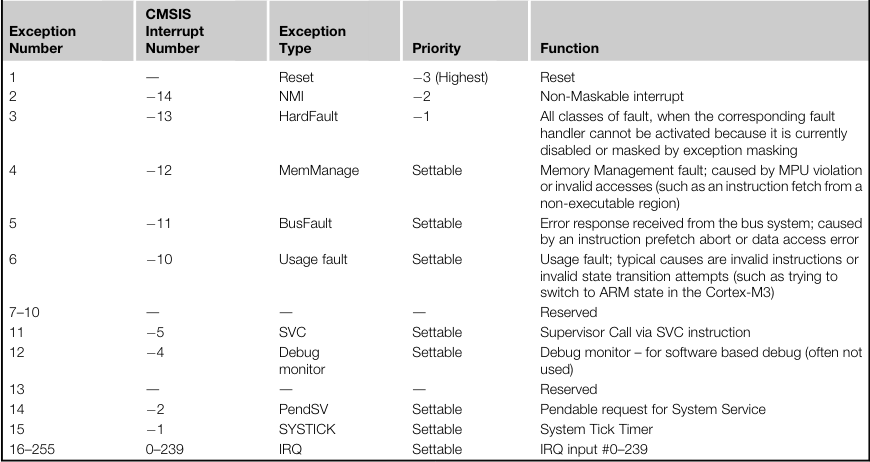
\includegraphics[width=0.95\textwidth]{./figures/ch1/cortex-m/exception-types.png}
  \end{center}
  \caption{Tabella delle eccezioni del Cortex M3/M4}\label{fig:cortex-m-exception}
\end{figure}

NVIC ha una \textit{Vector Table} (riportata in \cref{fig:cortex-m-vector-table}) in cui ci sono gli indirizzi di memoria a cui saltare per gestire le eccezioni. Questa tabella può essere caricata dall'utente per gestire le periferiche. Ad esempio, STM userà le interruzioni per integrare il core con i suoi dispositivi.

Essendo indirizzi a $32-bit$ gli ultimi $2-bit$ sono sempre zero. ARM sfrutta questo fatto per codificare se la \textit{routine} deve essere gestita in ARM o Thumb state. Infatti, nel Cortex-M (che non ha ARM state), LSB (bit più a destra, meno significativo) è sempre $1$.

\begin{figure}[H]
  \begin{center}
    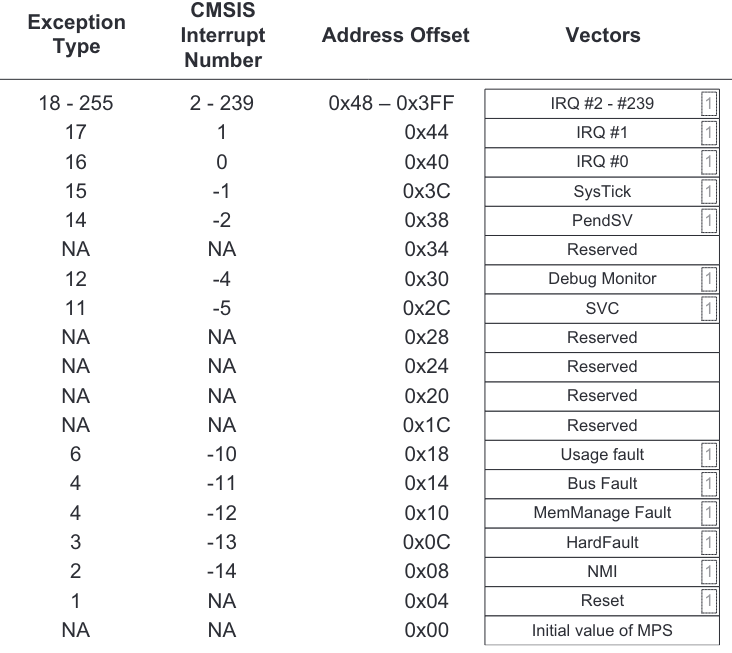
\includegraphics[width=.7\textwidth]{./figures/ch1/cortex-m/vector-table.png}
  \end{center}
  \caption{Indirizzi handler delle interruzioni in Cortex M3/M4}\label{fig:cortex-m-vector-table}
\end{figure}

\subsubsection{Memoria}
Sul Cortex-M, si hanno a disposizione $4GB$ di spazio lineare con indirizzi a $32-bit$ partizionata come in \cref{fig:cortex-m-memory-map}.

\begin{figure}[h]
  \begin{center}
    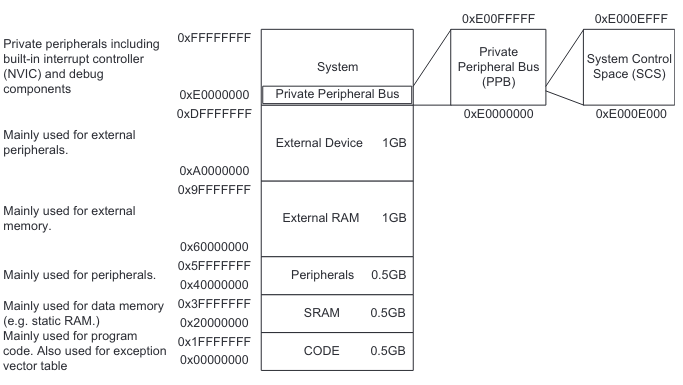
\includegraphics[width=0.95\textwidth]{./figures/ch1/cortex-m/memory-map.png}
  \end{center}
  \caption{Partizionamento della memoria nel Cortex-M}\label{fig:cortex-m-memory-map}
\end{figure}
\begin{itemize}
  \item \textbf{SYSTEM}: gestore delle interruzioni, timer, registri di controllo\dots;
  \item \textbf{External SRAM}: serve a fare il mapping con un eventuale dispositivo DRAM esterno;
  \item \textbf{SRAM}: in cui memorizzare l'accesso ai dati utilizzati dai programmi in CODE;
  \item \textbf{CODE}: in cui memorizzare i programmi utente;
  \item \textbf{External Peripherals}: è uno spazio dedicato a mappare le periferiche integrate da un vendor (come \textit{ST});
\end{itemize}

\begin{figure}[h]
  \begin{center}
    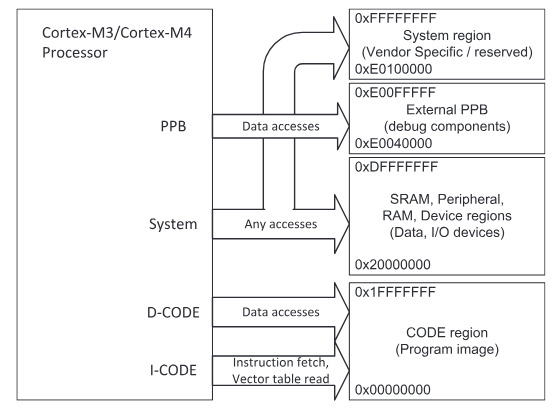
\includegraphics[width=0.65\textwidth]{./figures/ch1/cortex-m/memory-interface.png}
  \end{center}
  \caption{Interfacciamento con la memoria}\label{fig:cortex-m-memory-interface}
\end{figure}

Guardando la \cref{fig:cortex-m4-arch}, il \textit{core} si interfaccia con la memoria attraverso un componente \textbf{Interconnect}. Elimimando l'astrazione del componente interconnect, si può vedere la sua architettura in \cref{fig:cortex-m-memory-interface}. Ciascuna parte della memoria è acceduta utilizzando un bus (e un protocollo) diverso. Ad esempio, le periferiche interne possono essere accedute con \textbf{APB} attraverso il \textit{PPB} (Private Peripheral bus), quelle esterne con \textit{AHB} (AMBA High-performance bus). Un diagramma più dettagliato è mostrato in \cref{fig:cortex-m-memory-interface-detail}.

\begin{figure}[H]
  \begin{center}
    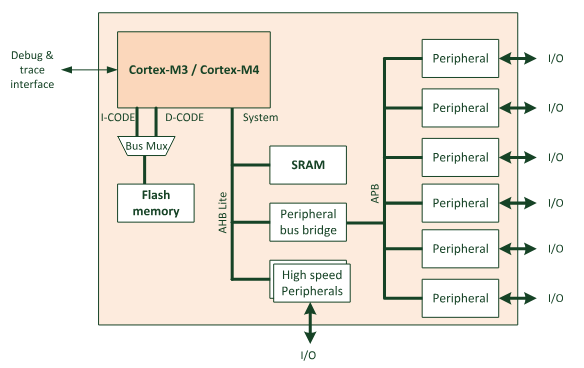
\includegraphics[width=0.75\textwidth]{./figures/ch1/cortex-m/memory-interface-detail.png}
  \end{center}
  \caption{Dettaglio interfacciamento con la memoria}\label{fig:cortex-m-memory-interface-detail}
\end{figure}

\paragraph{Bit-band region} Nei micro-controllori, molte operazioni sono fatte sui singoli bit di un registro (come ad esempio nel GPIO). Questo implica che oer fare il toggle di un bit bisogna leggere il registro, modificarlo e scriverlo (si crea un pattern \textit{read-modify-write}) che non è atomico e può creare problemi di consistenza. Il problema può essere risolto disabilitando le interruzioni, ma degradando di molto le prestazioni. ARM specifica un meccanismo detto \textbf{Bit-band}: crea un registro finto di $32-bit$ su cui vengono inseriti i singoli bit di altre regioni. In questo modo, gli accessi a bit differenti dello stesso registro è isolato. Questo è un meccanismo per controllare in maniera efficiente le periferiche esterne effettuando di fatto un \textit{alias}.

\paragraph{Alignment e endianess} ARM supporta sia la modalità big-endia che little endian. Tipicamente si usa la little-endian. L'accesso alla memoria può non essere allineato a $32-bit$ per la parte dati. Tuttavia ci sono alcuni casi speciali. Per le operazioni sullo stack (push e pop), load/store, operazioni esclusive e operazioni di tipo \textbf{Bit-band} gli accessi deveono essere allineati.

\paragraph{Attributi di memoria} Ad ogni regione di memoria sono associati 2 bit per configurare il comportamento di memoria e della cache (\textit{bufferable} e \textit{cacheable}), come in \cref{tab:memory-attributes}, e due per indicare che la memoria è \textit{executable} e \textit{shareable} 

\begin{table}
  \caption{Attributi di memoria nel Cortex-M}\label{tab:memory-attributes}
  \begin{center}
    \begin{tabular}[c]{l|l|l}
      \hline
      \multicolumn{1}{c|}{\textbf{Bufferable}} & 
      \multicolumn{1}{c|}{\textbf{Cacheable}} &
      \multicolumn{1}{c}{\textbf{Memory type and behavior}} \\
      \hline
      0 & 0 & \textbf{Strong ordered}: attendere del trasferimento\\
      1 & 0 & \textbf{Device type}: una scrittura può essere bufferizzata  \\
      0 & 1 & memoria con cache \textbf{write through} \\
      1 & 1 & memoria con cache \textbf{write back}\\
      \hline
    \end{tabular}
  \end{center}
\end{table}

\paragraph{Memory Protection Unit: MPU} L'MPU è un dispositivo che si intromette tra il core e l'interfacciamento con la memoria. Questo dispositivo può essere configurato con range di indirizzi e indicando quali sono le operazioni che devonoe essere eseguiti su di essi (\textit{read, write, executable}) e la modalità di privilegio in cui bisogna trovarsi. Bisgona notare che questo componente è opzionale e non è presente in tutti i Cortex-M.

Questo può essere utilizzato per creare una forma di protezione: un sistema operativo può proteggere le strutture dati da un task utente; oppure può essere usato per creare una forma di isolamento rudimentale. Quindi è una matrice che incrocia una serie di attributi e solleva un'eccezione di \textit{memory fault}.

\paragraph{Memory barriers} Anche nel Cortex-M, bisogna trattare problemi di consistenza verso la memoria considerando anche chi il core non conosce cosa succede nel memory controller. Infatti, il vendor potrebbe aggiungere una DRAM \textit{off-chip} che effettua operazioni di ottimizzazione delle transazioni e ciò potrebbe condurre a risultati non corretti. Una \textbf{memory barrier} è un meccanismo per dire al controller della memoria di \textit{prescindere da tutte le ottimizzazioni hardware propagando con certezza tutte le transazione iniziate} (\textit{out-of-order execution} non supportata da Cortex-M). La memory barrier viene implementata con $3$ istruzioni:
\begin{itemize}
  \item \textbf{DMB}: data memory barrier. Assicura che tutti gli accessi in memoria sono completati prima del successivo;
  \item \textbf{DSB}: data syncronization barrier. Assicura che tutti gli accessi in memoria sono completati prima prossima istruzione;
  \item \textbf{ISB}: instruction syncronization barrier. Effettua un flush della pipeline, assicurando che tutte le istruzioni sono completate prima delle prossime;
\end{itemize}

Con ARMv7, può sembrare eccessivo, ma con ARMv8 i processori Cortex-M sono complicati e se un RTOS deve fare un context switch allora è necessario ripulire tutto il core propagando i diversi tipi di cache.

\subsubsection{Infrastruttura di debug}
L'infrastruttura di debug (\cref{fig:cortex-m-debug-infra}) è un componente opzionale sia perchè viene solo utilizzato in fase di sviluppo sia perchè può essere un vettore di attacco visto che lascia completo accesso al dispositivo. Dopo la fase di sviluppo i connettori per il debug vengono bruciati per impedirne l'accesso. Infatti, attraverso il debugging si accede a strutture dati che non è possibile accedere da programmatore. Quindi l'infrastruttura di debug deve essere hardware e produce un blob di bit in uscita ed è necessario avere un indice (particolare per il modello della board) in cui è descritto il significato di ogni singolo bit.

Il protocollo standard per fare debugging è \textbf{JTAG}. Si tratta di un protocollo seriale con $5$ fili che scansiona (attraverso una \textbf{scan chain}) l'intero sistema. Quando il sistema è in modalità di debug, tutti i fli-flop entrano in una modalità di funzionamento (scan mode) tale per cui diventano l'n-esimo stadio di un grande shift register. Attraverso dei comandi, JTAG prevede le operazioni di base e quindi è possibile leggere il valore di tutti i registri nel sistema. Oltre a quella standard, ARM ha un'interfaccia di debug \textit{SWD} (\textbf{Serial Wire Debugging}) che è una reinterpretazione di JTAG e condividono anche gli stessi fili. Infine, c'è una terza interfaccia (questa volta parallela) detta \textit{TRACE}  che permette di estrarre dati dalla memoria, ma è qualcosa propost ed implementato solo da ARM.

\begin{figure}[h]
  \begin{center}
    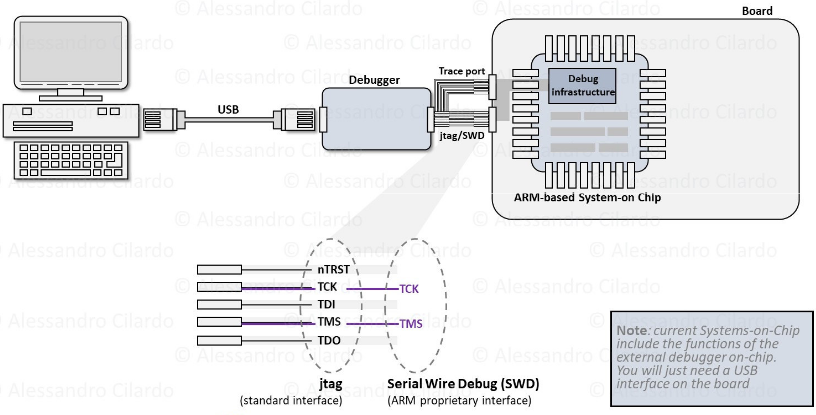
\includegraphics[width=0.95\textwidth]{./figures/ch1/cortex-m/debug-infra.png}
  \end{center}
  \caption{Infrastruttura di debug per il Cortex-M}\label{fig:cortex-m-debug-infra}
\end{figure}

Il protocollo JTAG utilizza un'interfaccia di debug e dei controller che vengono istanziati sui vari chip. JTAG funziona effettuando delle richieste ai controller creando una sola unica catena di scan che deve essere leggibile e scrivibile. Oltre a questo protocollo di basso livello, c'è un'infrastruttura di alto livello che serve a specificare a JTAG cosa possiede la scheda a cui è collegato e sostanzialmente quali sono le risorse su cui può accedere (memorizzando queste informazioni in una maniera standard).

\subsubsection{ARM Ethos Network Processing Unit (NPU)}
ARM Ethos è una serie di processori specializzati per l'accelerazione delle operazioni di intelligenza artificiale e machine learning, progettati per essere integrati in dispositivi embedded. Le caratteristiche peculiari di ARM Ethos includono:

\begin{itemize}
  \item \textbf{Efficienza energetica}: Progettati per offrire alte prestazioni con un consumo energetico ridotto, rendendoli ideali per dispositivi mobili e applicazioni IoT.
  \item \textbf{Supporto per reti neurali complesse}: Capaci di eseguire reti neurali convoluzionali (CNN), reti neurali ricorrenti (RNN) e altre architetture di deep learning con alta efficienza.
  \item \textbf{Scalabilità}: Disponibili in diverse configurazioni per adattarsi a una vasta gamma di applicazioni, dai dispositivi a bassa potenza ai sistemi ad alte prestazioni.
  \item \textbf{Integrazione con ARM Cortex}: Progettati per funzionare in sinergia con i processori ARM Cortex, facilitando l'integrazione nei sistemi esistenti.
  \item \textbf{Supporto per strumenti di sviluppo}: Compatibili con strumenti di sviluppo e framework di machine learning come TensorFlow Lite, facilitando lo sviluppo e l'ottimizzazione delle applicazioni AI.
\end{itemize}

\paragraph{Operazioni SIMD}
Nel contesto delle architetture ARM, le operazioni SIMD sono supportate dall'estensione NEON. NEON è un'unità di elaborazione avanzata che può eseguire operazioni su vettori di dati, tipicamente con lunghezze di 64 o 128 bit. Ogni vettore può essere suddiviso in elementi di 8, 16, 32 o 64 bit, permettendo operazioni parallele su questi elementi.

\begin{itemize}
  \item \textbf{Registri NEON}: NEON dispone di 32 registri a 64 bit (D0-D31) che possono essere accoppiati per formare 16 registri a 128 bit (Q0-Q15). Questi registri possono contenere vari tipi di dati, inclusi interi e floating-point.
  \item \textbf{Istruzioni SIMD}: Le istruzioni NEON includono operazioni aritmetiche, logiche, di spostamento e di confronto. Ad esempio, un'istruzione di somma vettoriale può sommare simultaneamente più coppie di numeri interi contenuti in due registri vettoriali.
  \item \textbf{Pipeline SIMD}: Le operazioni SIMD sono eseguite in una pipeline dedicata, separata dalla pipeline principale del processore. Questo permette di mantenere un alto throughput di elaborazione senza interferire con le operazioni scalar.
  \item \textbf{Caricamento e memorizzazione}: Le operazioni di caricamento e memorizzazione di dati nei registri NEON sono ottimizzate per gestire blocchi di dati contigui, riducendo il numero di accessi alla memoria e migliorando le prestazioni.
  \item \textbf{Interleaving e deinterleaving}: NEON supporta operazioni di interleaving e deinterleaving, che permettono di riorganizzare i dati nei registri vettoriali per ottimizzare l'elaborazione parallela.
\end{itemize}

L'uso delle operazioni SIMD con NEON può portare a significativi miglioramenti delle prestazioni in applicazioni che possono sfruttare il parallelismo a livello di dati, riducendo il tempo di elaborazione e migliorando l'efficienza energetica.

\clearpage
\subsection{Cortex-A}
Il Cortex-A è un processore di fascia alta in cui la A significa \textit{Application}. In generale, viene fatta un'analisi su ARMv7 (architettura a $32-bit$ evidenziando le differenze con ARMv8 (architettura a $64-bit$). 

\subsubsection{ARMv7}
Rispetto al Cortex-M, il Cortex-A supporta la doppia ISA \textit{ARM ISA} e \textit{Thumb2} (che può essere a $16$ o $32$ bit) e si focalizza su introdurre supporto a istruzioni SIMD con l'estensione vettoriale \textbf{NEON} attraverso un ALU con \textit{lane} dinamiche. 
Un elemento importante di ARMv7 è \textbf{Jazelle}: un supporto hardware della JVM che è una macchina a stack a $8-bit$. 

\paragraph{Modalità operative} Rispetto al Cortex-M con soli $3$ modalità operative, il Cortex-A ne prevede $7$ (in verticale in \cref{fig:cortex-a-banked-register}) :
\begin{itemize}
  \item User: modalità utente in cui esegue codice non privilegiato;
  \item System: modalità privilegiata in cui vengono usati gli stessi registri della modalità User;
  \item Abort: stato in cui si entra quando si verifica un fault relativo alla memoria (\textit{ie. page fault});
  \item Undef: stato in cui si entra quando non si riesce a decodificare un'istruzione;
  \item Supervisor: modalità che serve a fare i cambi di privilegio 
  \item IRQ: modalità in cui si servono le interruzioni ordinarie per le periferiche;
  \item FIQ: interruzioni per le periferiche che hanno requisiti di latenza.
\end{itemize}

\paragraph{Registri}
Il Cortex-A fa un forte utilizzo di \textbf{banked registers} per evitare di copiare troppe cose quando si effettua un cambio di contesto. Ogni modalità operativa ha il proprio PC, LR, ma per facilitare la condivisione i registri $R0-R3$ sono condivisi per velocizzare il passaggio di parametri.
L'idea è quella di effettuare meno push sullo stack, minimizzando gli accessi in memoria. Un registro che viene sicuramente salvato è il \textbf{\textit{CPSR} (curren program status register)} che viene salvato automaticamente \textbf{\textit{SPSR (saved program status register)}}.

Lo status register è molto simile a quello del Cortex-M e contiene:
\begin{itemize}
  \item $8-bit$ per l'uscita dell'ALU;
  \item bit $Q$ \textit{sticky}: per indicare l'aritmetica a saturazione;
  \item bit $J$: indica se si sta eseguendo in modalità Jazelle;
  \item bit $T$: per indicare quale ISA si sta eseguendo \textbf{Thumb/ARM};
  \item bit $E$: per indicare \textbf{\textit{endianess}};
  \item bit $FIQ$ $IRQ$: per abilitare le interruzioni fisiche;
  \item bit $SIMD$: bit in uscita dalla parte vettoriale;
  \item bit $Mode$: indicano la modalità operativa in cui ci si trova;
\end{itemize}

\begin{figure}[h]
  \begin{center}
    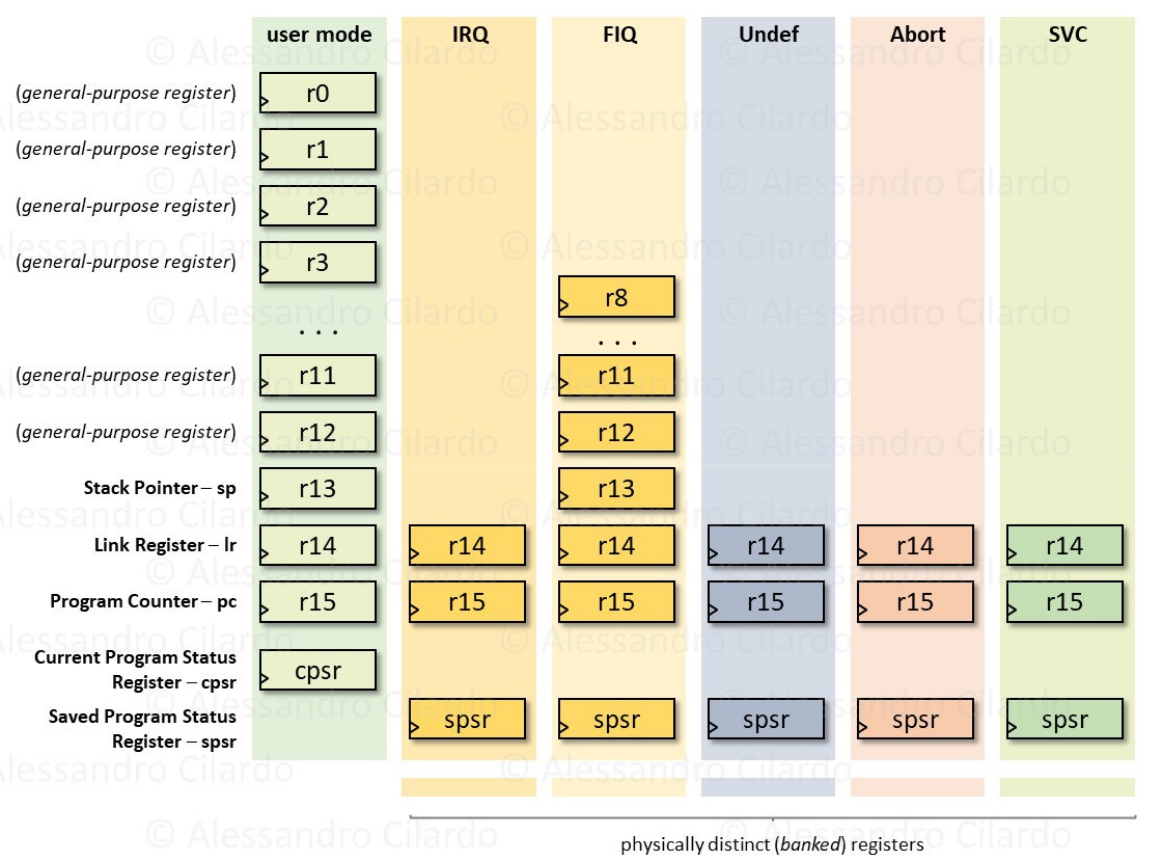
\includegraphics[width=.90\textwidth]{./figures/ch1/cortex-a/armv7-banked-register.png}
  \end{center}
  \caption{Register file per modalità operative}\label{fig:cortex-a-banked-register}
\end{figure}

Quando arriva un'eccezione, il core salva il CPSR in SPSR, viene configurato la nuova modalità e salta all'indirizzo dell'handler appropriato nella vector table (tutti gli altri registri sono mascherati con il cambio di modalità). Un caso particolare è la FIQ: viene sempre posizionato all'inizio della vector table in modo tale da poter eseguire alcune istruzioni prima di un branch per ridurre il tempo di risposta.

\paragraph{Memoria} Essendo un processore di fascia applicativa l'interfacciamento con la memoria può essere complicato. Infatti, i sistemi di fascia alta devono offrire supporto per la memoria virtuale, coerenza e consistenza. Il Cortex-A si integra con una load/store unit che può effettuare molte operazioni per ottimizzare l'accesso in memoria. Ad esempio, la load/store unit può riordinare le operazioni di lettura/scrittura facendo \textbf{\textit{coalescing}} per sfruttare al massimo il bus di interconnessione. Queste problematiche possono essere risolti disabilitando il \textit{caching}, \textit{transaction reordering} ecc.

Analogamente al Cortex-M, sono presenti attributi di memoria per specificare l'utilizzo della memoria:
\begin{itemize}
  \item \textbf{Normal}: è possibile effettuare operazioni di efficienza. È possibile decidere se un'area di memoria è condivisa e specificare gli attributi per la policy di caching;
  \item \textbf{Device}: un'area di memoria in cui si mappano registri delle periferiche. Bisogna disabilitare il caching poichè letture di un registro di periferica in cache porta risultati falsati;
  \item \textbf{Strongly ordered}: viene inibito qualsiasi riordine per non avere nessuna ottimizzazione;
\end{itemize}

\clearpage
\subsubsection{Cortex-A9}
Il cortex-A9 è un esempio di architettura ARMv7.  Come si vede dalla \cref{fig:cortex-a9}, include una parte di esecuzione speculative con \textit{prefetcher} e scrittura in memoria \textit{out-of-order}. Le caratteristiche principali sono il fetching di due istruzioni per volta e il \textit{dispatching} di fino a $4$ istruzioni per clock. Questo processore include un \textbf{return stack buffer} in cui viene copiato in automatico l'indirizzo di ritorno a funzione su chip.

Il prefetcher è in grado di prendere $8$ stream di dati indipendente continuando a mettere in cache L1 fino a quando riesce non incontra \textit{cache miss}.
\begin{figure}[h]
  \begin{center}
    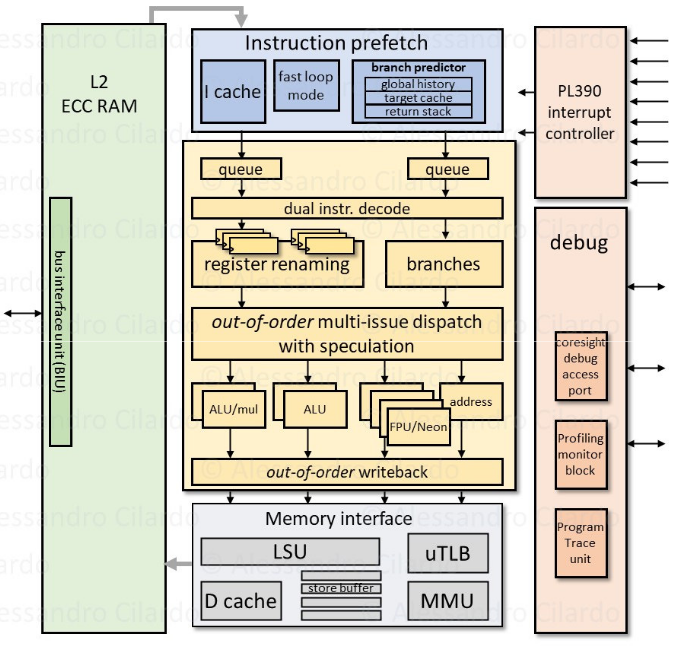
\includegraphics[width=.75\textwidth]{./figures/ch1/cortex-a/armv7-a9.png}
  \end{center}
  \caption{Architettura Cortex-A9}\label{fig:cortex-a9}
\end{figure}

Per la memoria virtuale, supporta due livelli di TLB (\textit{micro TLB} e \textit{main TLB}) separati per la parte dati e istruzioni.

\paragraph{Versione multi-core}
Questo processore può essere integrato fino ad avere $4$ core aggiungendo componenti per avere coerenza. In questa versione, i singoli \textit{core} hanno una cache L1 dedicata e una L2 condivisa. Il meccanismo per garantire la coerenza è una \textbf{snoop unit} (\cref{fig:cortex-a9-mcore}) che monitora tutte le transazioni con tag all'interno della cache L2. La snoop unit comunica con \textbf{\textit{Accelerator Coherence Port}} che consente a oggetti esterni di modificare il concetto di cache. 

In \cref{fig:cortex-a9-mcore}, è mostrato l'\textbf{\textit{Advanced Bus Interface Unit}}che consente di avere l'interconnessione della periferica sia su silicio che con un FPGA.

Ad esempio, è possibile avere un coprocessore su FPGA che accede a dei dati mappati nello spazio di indirizzamento dell'host. Il protocollo di coerenza non viene invocato nel momento in cui è l’unità esterna (es.: core FPGA) ad accedere a questa regione di memoria. Ciò comporta che i dati nella cache dei core risultano essere diversi presenti in memoria quando modificati da un’entità esterna.
Con l'utilizzo dell’ACP è possibile invalidare le linee di memoria del buffer esterno cachate e così sfruttare il meccanismo di coerenza per recuperare forzatamente i dati dalla memoria esterna, piuttosto che utilizzare i dati salvati in cache. Consente quindi di invalidare delle copie di finestre di memoria di un acceleratore che possono essere modificate da entità esterne (da cui il nome dell’unità)

\begin{figure}[h]
  \begin{center}
    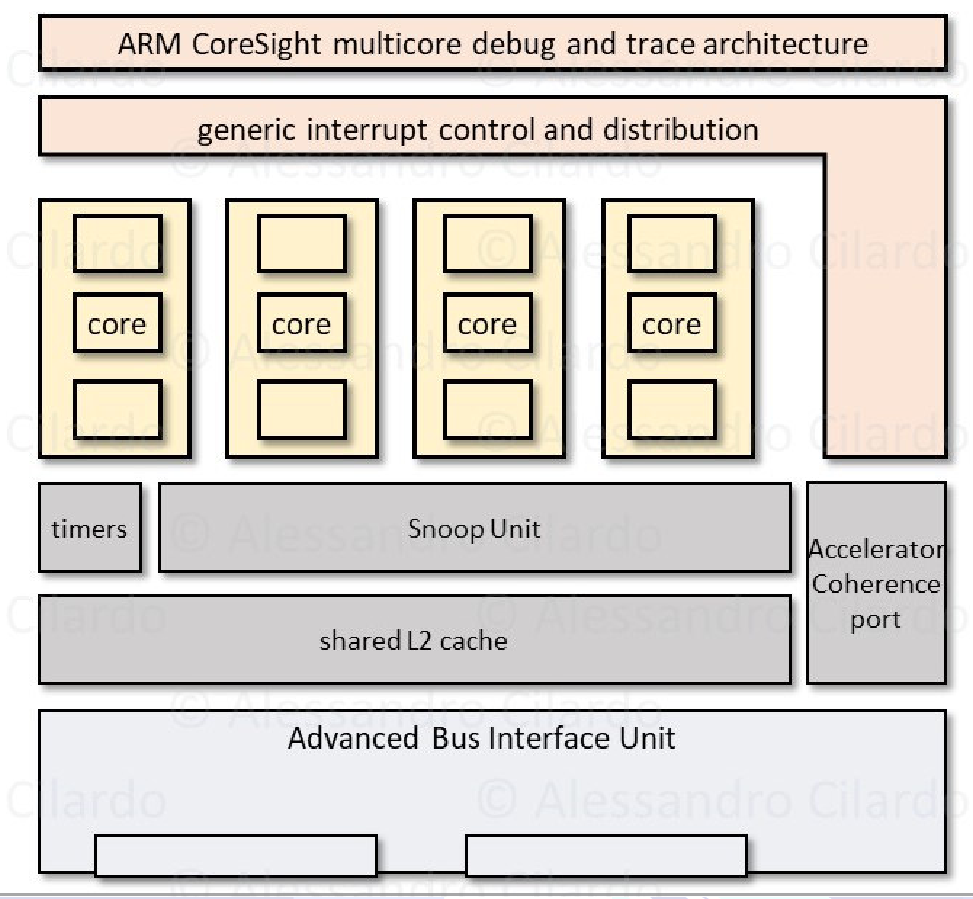
\includegraphics[width=.6\textwidth]{./figures/ch1/cortex-a/armv7-a9-multicore.png}
  \end{center}
  \caption{Componenti aggiuntivi per Cortex-A9 in versione multi-core}\label{fig:cortex-a9-mcore}
\end{figure}

\subsubsection{ARMv8}
ARMv8 supporta sia ISA a $32-bit$ che a $64-bit$ e rimuove alcuni meccanismi da ARMv7 che sono stati ritenuti inefficaci. Ad esempio, ARMv7 supporta istruzioni con pattern del tipo \textbf{\textit{ITxxx} (if-then-else)}. Inoltre, supporta la possibilità di disabilitare la cache e supporto esplicito per alcune applicazioni come la crittografia (come ad esempio AES o SHA).

\paragraph{Registri}
ARMv8 ha $32$ registri a $64-bit$ indicati con $Xi$ $(X0-X31)$ di cui possono essere indicati essere indirizzabiti i $32-bit$ meno significativi con $W0-W31$. Ci sono i soliti registri speciali $X30/LR$ e con $SP/ZERO$. $X31$ è un registro speciale che si comporta da \textit{stack pointer} quando viene utilizzato come base per \textit{load/store}; mentre serva da \textit{zero register} quando viene utilizzato come sorgente o scarta il risultato di un'operazione quando viene usato come destinazione. $X30$ si occupa di agire da \textit{link register} e non è più \textit{banked} come in ARMv7.

\paragraph{Modalità operative} 
ARMv8 introduce un modello diverso di gestire le eccezioni detti \textbf{exceptio level}. Nella configurazione base sono presenti $4$ exception level rappresentati in \cref{fig:armv8-base-exception-level}.
\begin{itemize}
  \item \textbf{\textit{EL0}}: livello utente con meno privilegi;
  \item \textbf{\textit{EL1}}: livello dedicato al sistema operativo;
  \item \textbf{\textit{EL2}}: livello dedicato al hypervisor;
  \item \textbf{\textit{EL3}}: livello dedicato al \textit{firmware} e \textit{security code};
\end{itemize}
Esistono due tipi di privilegi:
\begin{itemize}
  \item \textbf{\textit{Memory}}: attributi di memoria configurati nel MMU differenziati tra EL0 e EL1-EL3;
  \item \textbf{\textit{System Registers}}: definiscono il contesto del processore che controllano caratteristiche dell'harware come spazi di indirizzi, configurazione MMU ecc;
\end{itemize}

\begin{figure}[h]
  \begin{center}
    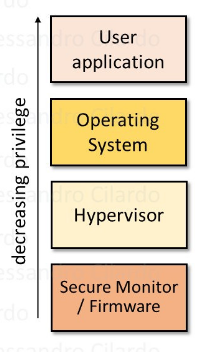
\includegraphics[width=.2\textwidth]{./figures/ch1/cortex-a/armv8-base-exception-level.png}
  \end{center}
  \caption{Livelli di privilegio in ARMv8}\label{fig:armv8-base-exception-level}
\end{figure}

In \cref{fig:armv8-exception-level}, è mostrata un'ulteriore divisione in verticale degli exception level. In particolare, ARMv8 introduce l'implementazione di un \textbf{Trusted Execution Environment} attraverso il meccanismo dei \textit{security states}. Tutto quello visto fino a questo momento fa parte del security state \textbf{non-secure}. Ad esempio, sono presenti alcune strutture dati e aree di memoria accessibili sono mentre si è in \textbf{secure state} (incluso il passaggio di stato) come registri speciali, interruzioni sicure ecc.

C’è un’ulteriore distinzione tra \textbf{AArch32} \textbf{AArch64} nei diversi EL. In realtà, non c’è ortogonalità tra aarch32 e aarch64 ma un principio di unidirezionalità: può accadere che un EL più basso (tipo EL0) esegua a 32 bit e che il livello cambi verso 64 bit nei livelli più alti, ma non è concesso il contrario. Questo perché un’applicazione utente a $32-bit$ esegue su un sistema operativo a $64-bit$. Non è possibile che un’applicazione utente a $64-bit$ esegua su un OS a $32-bit$. La regola generale è che il livello di eccezione può crescere contestualmente con il EL, e questo vale anche quando si passa verso il livello EL2 (tra VM e hypervisor).

\begin{figure}[ht]
  \begin{center}
    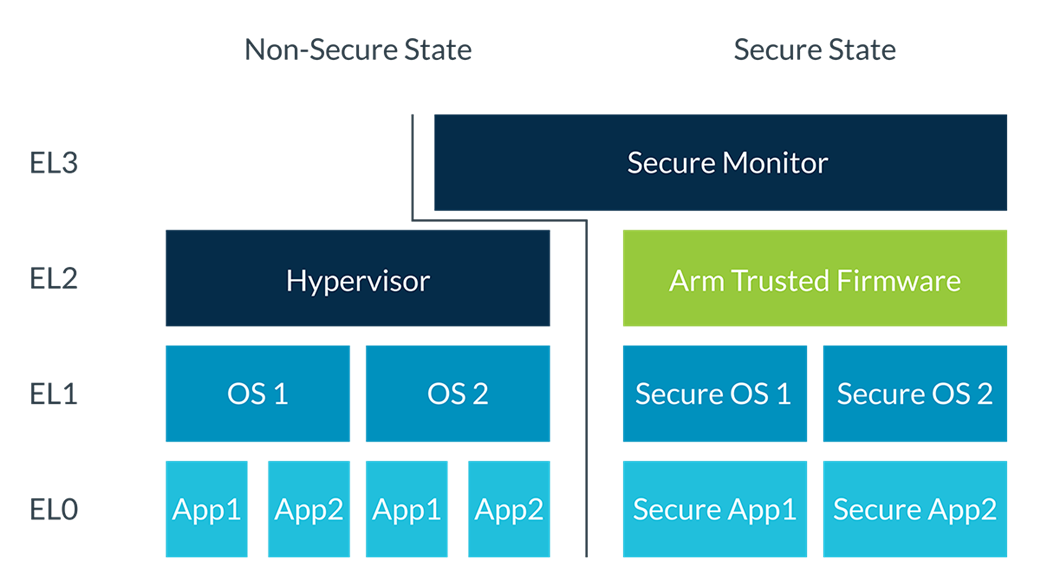
\includegraphics[width=.8\textwidth]{./figures/ch1/cortex-a/armv8-exception-level.png}
  \end{center}
  \caption{Modello di eccezione avanzato in ARMv8}\label{fig:armv8-exception-level}
\end{figure}

\paragraph{Gestione delle eccezioni}
Le gestione delle eccezioni è molto complicata perchè bisogna gestire la parte di virtualizzazione. Partendo dalla parte semplice, le eccezioni sono sempre di due tipi:
\begin{itemize}
  \item Sincrone: relative all'interno del processore (accessi di memoria invalid, istruzioni invalidi, problemi di privilegio ecc);
  \item Asincrone: relative alle periferiche. Queste possono essere sia fisiche che rivolte a macchine virtuali (e quindi devono essere inoltrate). ARMv8 mantiene FIQ e IRQ, ma le utilizza per effettuare una differenziazioni tra interruzioni relative al \textit{secure state} e \textit{non secure state}.
\end{itemize}

Quando si verifica un'eccezione il registro di stato viene salvato nel registro \textit{SPSR\_ELx} e l'indirizzo di ritorno dell'eccezione viene messo in \textit{ELR\_ELX} dedicato al livello di eccezione. $EL0$ è sprovvisto di questi registri perchè non può subire interruzioni.

L'handler che gestisce nelle eccezioni non è unico: ogni handler va duplicato per ogni exception level. In ARMv8, bisogna capire chi deve eseguire l'handler body e se l'interruzione deve essere inviata ad una macchina virtuale. Questo implica la presenza di un \textbf{\textit{top level handler}} che effettua alcune operazioni preliminari prima di gestire l'eccezione: salvare il tipo di eccezione, popolare alcuni registri e poi fare un salto al \textit{handler body} (anche in base a se l'handler deve essere a $32-bit$ o a $64-bit$) (\cref{fig:armv8-exc-handling}). Quindi il \textit{top level handler} contiene istruzioni e non un indirizzo a cui saltare. In particolare, contiene $128-byte$ di istruzioni. A differenza di come accade in architetture semplici come il Motorola, non hanno univocamente uno stack di modalità, ma hanno accesso allo stack della modalità interrotta e quello della propria, e questo può essere configurato.

\begin{figure}[ht]
  \begin{center}
    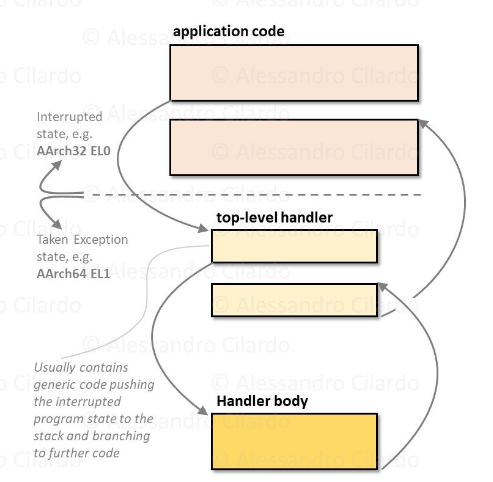
\includegraphics[width=.5\textwidth]{figures/ch1/cortex-a/armv8-exception-handling.png}
  \end{center}
  \caption{Gestione delle eccezioni in AArch64}\label{fig:armv8-exc-handling}
\end{figure}
\clearpage

La \textbf{\textit{vector table}} (\cref{fig:armv8-cortex-a-vector-table}) può essere divisa in $4$ regioni per gestire le interruzioni in base alla modalità in cui ci strova con handler a $128-byte$. La duplicazione viene fatta anche per migliorare le prestaizoni senza andare a riscrivere codice. La tabella delle interruzioni è rilocabile e dipende dal registro \textit{VBAR\_ELn}.

\begin{figure}[ht]
  \begin{center}
    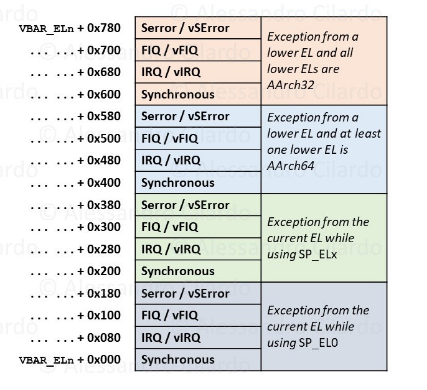
\includegraphics[width=.5\textwidth]{figures/ch1/cortex-a/armv8-vector-table.png}
  \end{center}
  \caption{Vector table di ARMv8 Cortex-A}\label{fig:armv8-cortex-a-vector-table}
\end{figure}

ARMv8 specifica un controller di interruzioni esterno ai core: \textbf{\textit{GIC (Generic Interrupt Controller)}} (\cref{fig:armv8-gic-arch}). Il GIC prevede tante interfacce quante sono le CPU, ognuna con due uscite, una IRQ e una FIQ oltre ad un livello comune detto \textbf{\textit{Distributor}} riceve diverse sorgenti di interruzioni, applica diversi criteri di masking delle priorità, e instrada verso l’opportuna interfaccia della CPU l’interruzione. Questo comportamento può essere largamente customizzato, configurato, usando dei registri di controllo/stato. Tra questi registri, in particolare di stato, c’è
quello che può essere letto da sw in particolare dal top level handler per andare a vedere qual è la sorgente di un’interruzione. In ARMv8, un'eccezione può essere in $4$ stati:
\begin{itemize}
  \item Inactive:  segnale basso
  \item Pending: segnale arrivato al GIC, ma ancora non  inoltrato all CPU;
  \item Active: handler in esecuzione;
  \item Active e Pending: quando un'interruzione è in esecuzione, ne arriva una dello stesso tipo. È possibile gestire interruzioni innestate;
\end{itemize}

\begin{figure}[ht]
  \begin{center}
    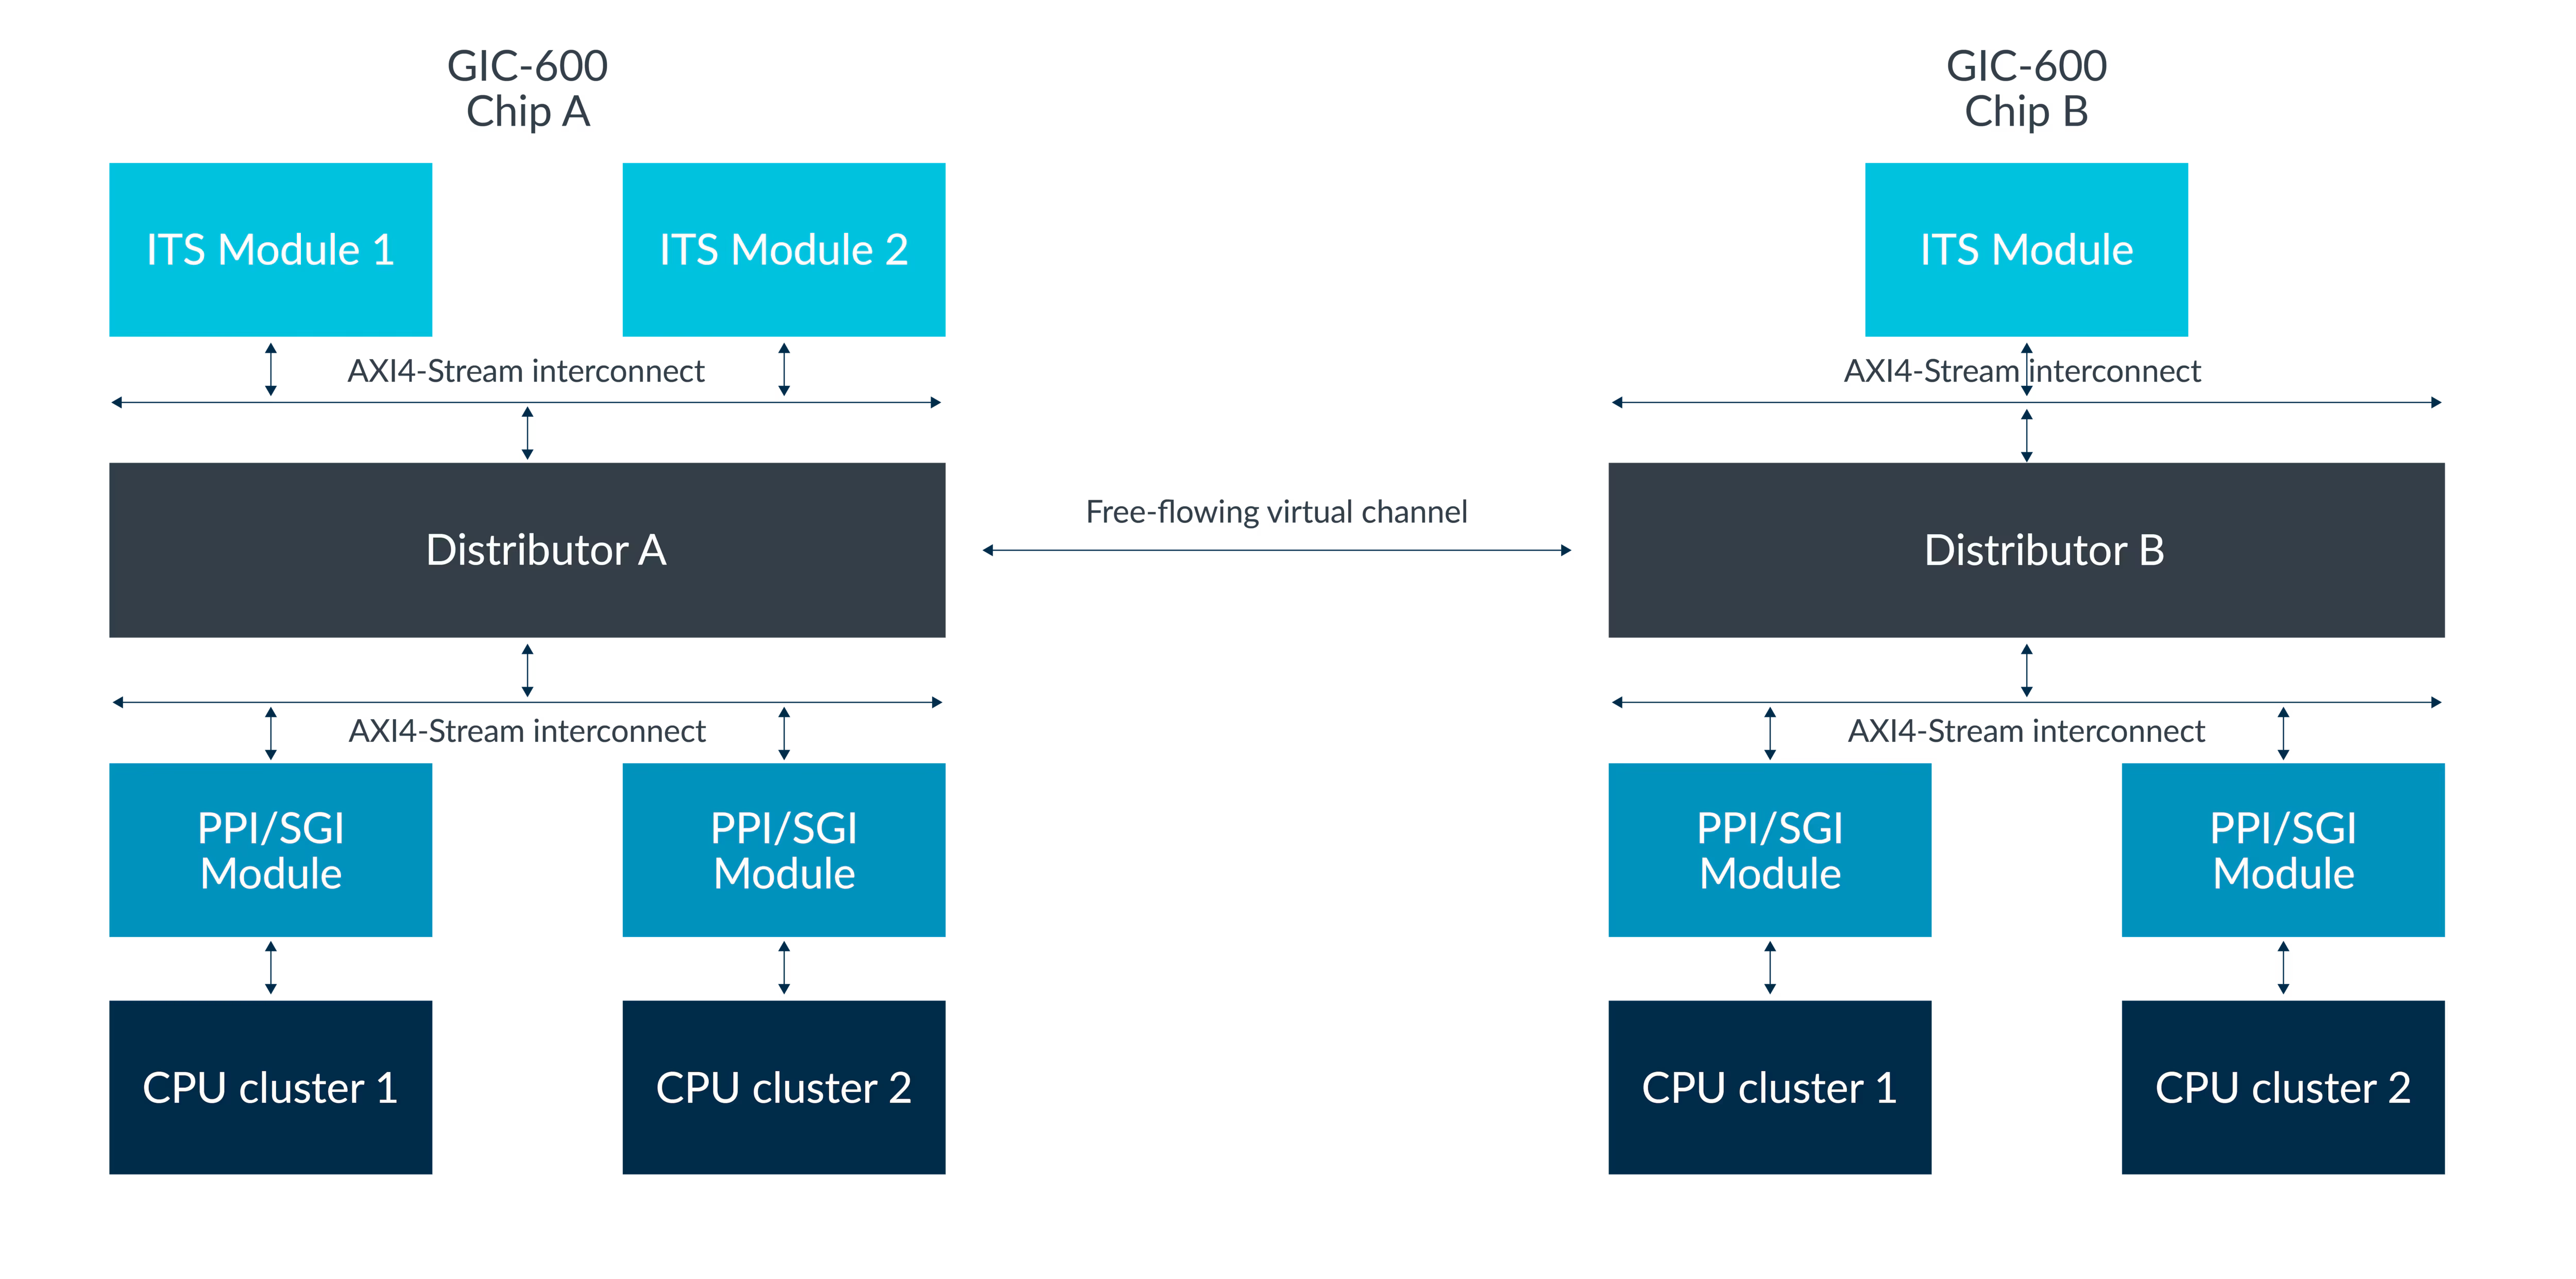
\includegraphics[width=.75\textwidth]{figures/ch1/cortex-a/armv8-gic.png}
  \end{center}
  \caption{Esempio di GIC in ARMv8}\label{fig:armv8-gic-arch}
\end{figure}

Quello che succederà quindi è che dall’esterno entreranno un certo numero di fili (numero definito dall’architettura del GIC) e dentro al GIC un registro che permette di sapere quali di questi fili sia alzato (\textit{IAR (Interrupt acknowledge register)} ed è il registro che il \textit{top-level handler} (uno dei $4$ nella vector table che può essere invocato) legge e sceglie l’opportuno handler da invocare. Un altro registro è quello con il quale si resetta lo stato dell’eccezione e si riporta allo stato di inactive: \textit{EOI (End of Interrupt)} scritto dal \textit{top-level handler}. 

A partire dalla versione $2$ del GIC, in maniera hardware, prevede la possibilità di registrare \textbf{virtual CPU interface} che consentono di gestire con la stessa logica fisica interruzioni per macchine virtuali. Questa operazione la effettua un'hypervisor in \textbf{EL1} quando registra una nuova VM. 

\paragraph{Gestione della memoria}
ARMv8 deve supportare un sistema operativo come Linux quindi memoria virtuale e per farlo si utilizza TLB. Dal punto di vista più basilare, un TLB è una \textit{black box} in cui si entra con un indirizzo virtuale e si esca con uno fisico. Estendendo il discorso ad ARM, la TLB si trova all'interno della MMU e si interpone tra il \textit{core} e la \textbf{\textit{cache}}. 

La TLB si comporta da cache poichè conserva solo le ultime traduzioni: in caso di miss entra in gioco un altro componente della MMU ovvero la \textbf{Table Walk Unit} che va ad interrogare la tabella dell pagine del processore in cui l'indirizzo virtuale è diviso in due parti: una indica il numero di pagina e l'altra l'offset della pagina. La granularità della traduzione è data dal numero di bit dell'offset e, vedendo la \cref{fig:armv8-tlb-mmu}, ogni blocco di memoria ha associato una serie di attributi che danno indicazioni su come gestirlo (eseguibile, \textit{read-only}, scrittura consentita ecc..)

\begin{figure}[ht]
  \begin{center}
    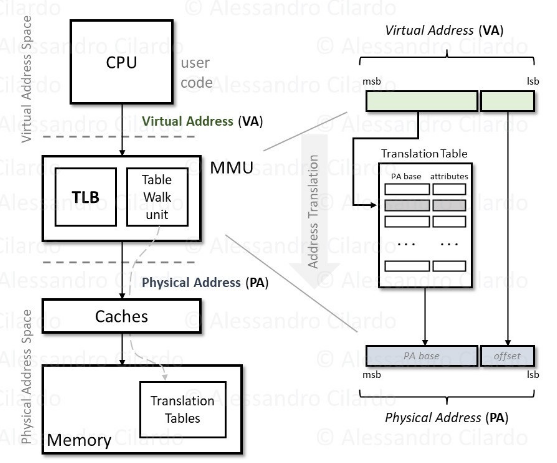
\includegraphics[width=.55\textwidth]{figures/ch1/cortex-a/armv8-tlb-mmu.png}
  \end{center}
  \caption{Funzionamento memoria virtuale in ARMv8}\label{fig:armv8-tlb-mmu}
\end{figure}

Nei sistemi moderni, la granularità fissa non funziona molto bene: alcune applicazioni hanno bisogno di gestire alcune aree di memoria in maniera fine. Per questo motivo, si introduce la \textbf{multi-level translation} (\cref{fig:armv8-multi-level.png}). ARMv8 arriva fino a $4$ livelli di traduzione con $3$ livelli di granularità diversi. La traduzione avviene a più fasi: ogni tabella contiene indicazioni per la prossima fino ad arrivare a quello fisico. Ciò diventa ancora più complicato con la virtualizzazione: questo processo funziona con un solo sistema operativo nel sistema.

\begin{figure}[ht]
  \begin{center}
    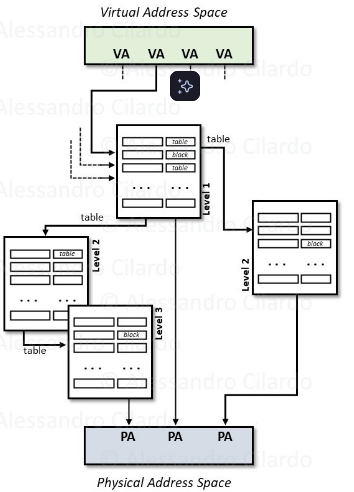
\includegraphics[width=.4\textwidth]{figures/ch1/cortex-a/armv8-tlb-multi-level.png}
  \end{center}
  \caption{Traduzione a più livelli}\label{fig:armv8-multi-level.png}
\end{figure}
 
In \cref{fig:multi-level-per-granule}, viene presentata una tabella in cui sulle colonne presenta quanto è grande l'offset e sulle righe i livelli di tabelle di traduzione.

\begin{figure}[bt]
  \begin{center}
    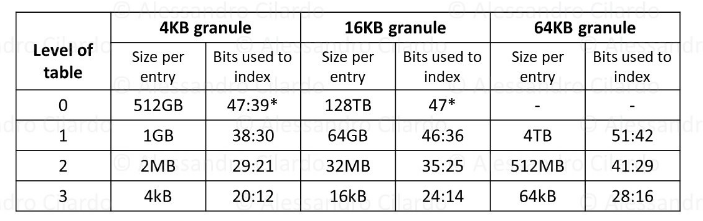
\includegraphics[width=.85\textwidth]{figures/ch1/cortex-a/armv8-tlb-multi-level-granule.png}
  \end{center}
  \caption{Memoria indirizzabile facendo variare livello di traduzione e granello}\label{fig:multi-level-per-granule}
\end{figure}

Con riferimento alla \cref{fig:multi-level-trans-ex}, da destra i primi $12-bit$ per l’offset ad esempio, altri $13-bit$ per l’accesso alla tabella di livello $3$, altri $9-bit$ per la tabella di livello $2$ e così via. Questo permette anche di fare una sorta di speculazione, nel senso che ci sono tabelle che vengono accedute più di frequente posso pensare di iniziare ad accedervi mentre intanto verifico che sia quella la tabella a cui devo accedere con gli altri bit del \textit{virtual address}. Tutto questo attiene semplicemente al meccanismo di traduzione degli indirizzi/gestione della memoria virtuale senza virtualizzazione.

\begin{figure}[H]
  \begin{center}
    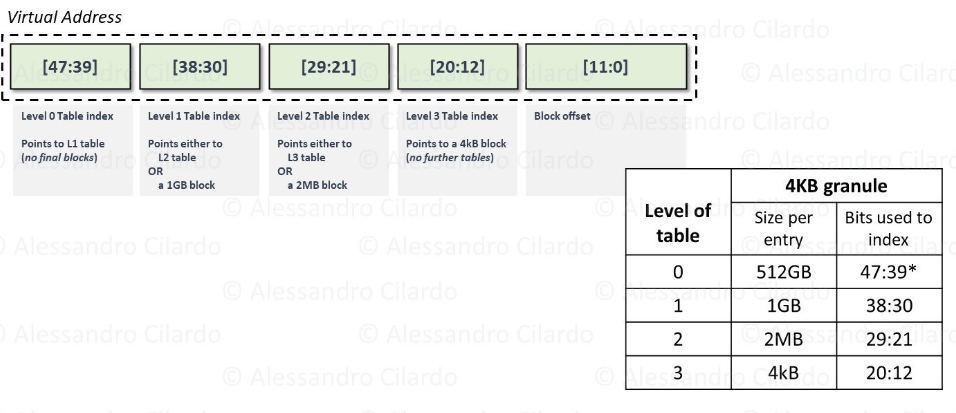
\includegraphics[width=.95\textwidth]{figures/ch1/cortex-a/armv8-tlb-multi-level-granule-example.png}
  \end{center}
  \caption{Esempio di partizionamento di un indirizzo virtuale}\label{fig:multi-level-trans-ex}
\end{figure}


\clearpage
\subsection{Interconnessioni e protocolli di comunicazione}
In questa sezione, saranno analizzati i protocoll di comunicazione con le periferiche. In particolare, si farà un focus su:
\begin{itemize}
  \item Serial Peripheral Interfae: SPI;
  \item Controller Area Network: CAN;
  \item Universal Serial Bus: USB;
  \item ARM Microcontroller Bus Architecture: AMBA;
\end{itemize}

Le periferiche sono un modo del SoC per interagire con il mondo esterno. Alcune di queste sono già presenti all'interno come memoria, controller ethernet ecc; altre devono essere integrate fisicamente utilizzando un \textbf{PHY}: un adattattore fisico che deve essere necessariamente esterno perchè opera con livelli elettrici diversi da quelli del SoC.

\subsubsection{Serial Peripheral Interfae: SPI}
SPI è un protocollo seriale di tipo \textit{master-slave} adatto per brevi distanze molto semplice. Escluse le alimentazioni $VCC$ e $GND$, ci sono $4$ fili in totale:

\begin{itemize}
  \item \textbf{SPI Clock}: segnale di clock di sincronizzazione;
  \item \textbf{Chip Select}: segnale di selezione dello slave. Ci sono tanti segnali (fili), quanto sono gli slave;
  \item \textbf{\textit{Master in Slave out (MISO)}}: dati che vanno dallo slave al master;
  \item \textbf{\textit{Master out Slave in (MOSI)}}: dati che vanno dal master allo slave;
\end{itemize}
Il protocollo è full-duplex, quindi questi due segnali sono usati in maniera contemporanea. Il singolo master ha $4$ segnali di uscita, ogni slave ha un proprio MISO che esce, e l’arbitraggio tra questi segnali può essere fatto in maniera diversa, ma di solito viene realizzato prevedendo che lo slave che non è abilitato, quindi con il chip select basso, ha il segnale di uscita MISO in alta impedenza. 

Dal punto di vista pratica, \textit{master} e \textit{slave} sono basati su \textbf{shift register} utilizzato per estrrare o inserire dati con una seriale (\cref{fig:spi-connection}).

\begin{figure}[h]
  \begin{center}
    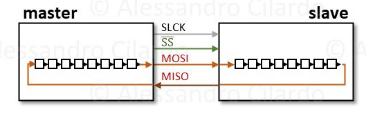
\includegraphics[width=.4\textwidth]{figures/ch1/protocols/spi-connection.png}
  \end{center}
  \caption{Interazione base tra \textit{master} e \textit{slave} con SPI creando uno shift register logico}\label{fig:spi-connection}
\end{figure}

Per il modo molto semplice con cui comunica, SPI prevede due modalità di collegamento con gli slave.

\paragraph{Slave in parallelo}
Tutti gli slave sono collegati al master attraverso un \textbf{chip select} dedicato (\cref{fig:spi-parallel-connection}. In pratica si realizza un \textbf{bus condiviso}, gli slave che non utilizzano devono mettere la propria uscita (MISO) in alta impedenza per evitare conflitti. Il segnale MOSI sarà portato per ogni slave.

\begin{figure}[H]
  \begin{center}
    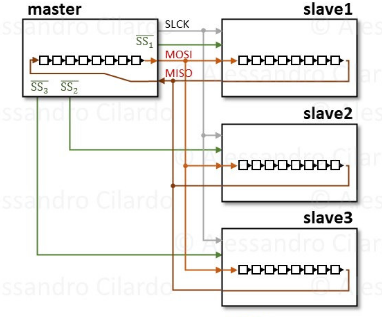
\includegraphics[width=.4\textwidth]{figures/ch1/protocols/spi-parallel-connection.png}
  \end{center}
  \caption{Connessione degli slave in parallelo con il master}\label{fig:spi-parallel-connection}
\end{figure}

\paragraph{Slave in serie}
Un altro modo di collegare gli slave è quello di metterli in serie collegando solo il primo slave al master e i restanti in cascata (\cref{fig:spi-serial-connection}). Si nota che normalmente l’implementazione di questo protocollo prevede che internamente le interfacce verso SPI sono degli shift register, in cui metto dati fatti da più bit che immetto all’esterno in modalità seriale. Infatti, una tipica implementazione di Spi, considerando una coppia singola di MOSI e MISO, ho in entrambi degli shift register che fanno scorrere i bit da sinistra verso destra. Questo comportamento è simile a quanto visto per il procotollo JTAG. 

Lo svantaggio di questi approccio è il tempo di propagazione.
\begin{figure}[H]
  \begin{center}
    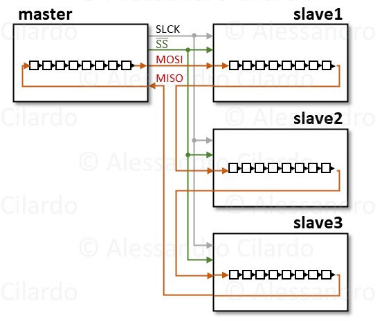
\includegraphics[width=.4\textwidth]{figures/ch1/protocols/spi-serial-connection.png}
  \end{center}
  \caption{Connessione in cascata degli slave}\label{fig:spi-serial-connection}
\end{figure}

\subsubsection{Controller Area Network: CAN}
CAN è un protocollo seriale a bus condiviso sincrono (tutti i dispositivi hanno lo stesso clock) nato per migliorare SPI ed essere adottato in ambito automotive. Il nuovo requisito di robustezza implica che bisogna gestire gli errori a livello fisico. Il protocollo supporta sia alte velocità (\textbf{1Mbps}) che basse (\textbf{50kbps}) e consente solo comunicazioni in \textbf{braodcast} (un nodo può decidere di ignorare un messaggio).

\paragraph{Segnali ed arbitraggio}
Lo scenario è che ci sono $n$ ECU che utilizzano due segnali $CAN_{high}$, $CAN_{low}$ che funzionano con una logica differenziale: se $CAN_{high} > CAN_{low}$ viene trasmesso $1$. Essendo un protocollo \textbf{multi-master} tutti possono iniziare una comunicazione e pertanto è necessario arbitrare l'accesso in scrittura. Per fare ciò si utilizza, un meccanismo $1-debole$: quando un \textit{tranceiver} vuole interagire comincia ad inviare il proprio id e, avendo lo zero priorità, la priorità massima sarà data al dispositivo con identificativo minore (con più zeri). Tutto questo si basa sulla presenza di una rete \textbf{\textit{carrier sense}} in cui chi invia il proprio identificativo ascolta per vedere se sta ricevendo il proprio id, se non è così smette di trasmettere.

\paragraph{Formato di un frame}
Dopo aver inviato l'identificativo, ci sono alcuni bit di sinccronizzazione. Non essendoci un \textbf{baud rate} fissato, bisogna sincronizzarsi con il \textbf{bit starting}. Successivamente, viene inviato \textbf{frame} vero e proprio. 

Esistono $3$ tipi di frame:
\begin{itemize}
  \item Data frame: utilizzati per inviare dati;
  \item Remote frame: utilizzati per ricevere dati;
  \item Error frame: utilizati per inviare errori;
\end{itemize}

I campi elencati in \cref{fig:can-frame-structure} sono:
\begin{itemize}
  \item Start of Frame: indica l'inizio di una trasmissione ($1 bit$);
  \item Arbitration field: identificativo del nodo ($11 bit$);
  \item Control field: lunghezza del payload o info sul payload ($6 bit$);
  \item Data field: payload del messaggio (da $0$ a $8$ bit);
  \item CRC field: controllo di ridondanza ($16 bit$);
  \item ACK field: indica se il messaggio è stato ricevuto ($2 bit$);
  \item End of Frame: indica la fine del frame ($7 bit$);
\end{itemize}

\begin{figure}
  \begin{center}
    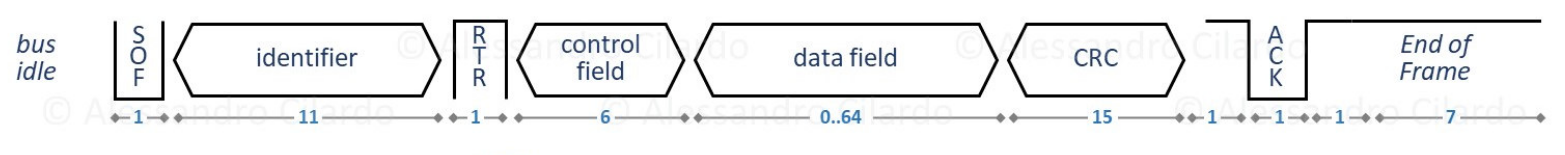
\includegraphics[width=0.95\textwidth]{figures/ch1/protocols/can-frame-structure.png}
  \end{center}
  \caption{Struttura di un frame CAN}\label{fig:can-frame-structure}
\end{figure}

Il protocollo CAN prevede $5$ tipologie di errore:
\begin{itemize}
  \item Bit error: ad esempio il bit RTR è 0 invece che 1;
  \item Stuff error: il protocollo proibisce di inviare $5-bit$ uguali per problemi di sincronizzazione;
  \item CRC error: payload corrotto;
  \item Form error;
  \item ACK error;
\end{itemize}

CAN ha un meccanismo per confinare gli errori per la \textbf{reliability}. Quando c'è un errore, viene inviato un apposito frame e il nodo cambia il suo stato interno. I nodi mantengono $2$ contatori per tenere traccia degli errori inviati (\textbf{Receive Error Counter (REC)}) e \textbf{Transmit Error Counter (TEC)}. Lo standard prvede dopo le soglie di $128$ e $256$. Oltre la prima soglia, si va in uno dei due specifici stuff error, mentre oltre la seconda si va in \textbf{bus off}, si smette di far funzionare il bus (automa in \cref{fig:can-error-fsm}).

\begin{figure}[H]
  \begin{center}
    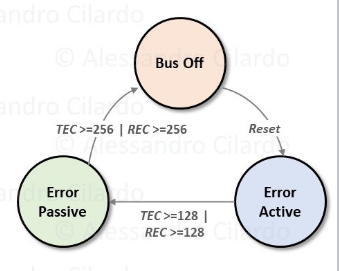
\includegraphics[width=.3\textwidth]{figures/ch1/protocols/can-error-fsm.png}
  \end{center}
  \caption{Gestione del numero di errori nel protocollo CAN}\label{fig:can-error-fsm}
\end{figure}

\subsubsection{Universal Serial Bus: USB}
Protocollo seriale disponibile in varie versioni: le ultime raggiungono velocità di $10 GB/s$ (\cref{fig:usb-evolution}). Il protocollo USB permette a due dispositivi di comunicare tra loro identificandosi come master o slave (\textbf{device} nel protocollo USB) attraverso una fase di \textit{handshaking}. Questo meccanismo, detto \textbf{\textit{USB On-The-GO (USB OTG)}} permette ai dispositivi di comunicare anche senza la presenza di un PC cambiando dinamcamente il proprio ruolo. Inoltre, USB serve sia per scambio dati che alimentazione. Anche in modalità OTG, USB rimane un protocollo master/slave in cui ci sono gli \textbf{host} (dispositivo che ha un hub USB) che agiscono come \textit{master} e i \textbf{device} (dispositivo che si connette all'hub) come \textit{slave}.

\begin{figure}[h]
  \begin{center}
    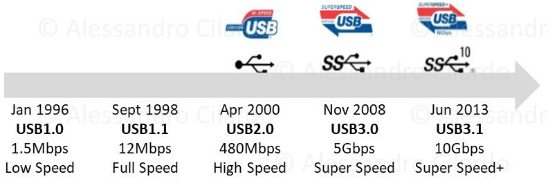
\includegraphics[width=.6\textwidth]{figures/ch1/protocols/usb-evolution.png}
  \end{center}
  \caption{Evoluzione del protocollo USB negli anni}\label{fig:usb-evolution}
\end{figure}

Il protocollo offre una funzionalità \textbf{\textit{hot plug}}: ogni dispositivo che si collega ad un master ha la possibilità di negoziare un indirizzo (a $7-bit$). L'architettura è molto semplice, un master fa polling sugli e costruisce dinamicamente la topologia di \textit{device}. L'indirizzo composto da tutti $0$ è speciale e serve a riconoscere un dispositivo in attesa di identificativo. Un altro indirizzo speciale è quello per il master, quindi nella topologia (detta \textbf{\textit{tiered star}}) sono supportati $126$ dispositivi. 

I controller host USB possono essere presenti sulla \textit{motherboard} di un PC o essere comprati esternamente. Possono essere alimentati fino a $500mA$ (esternamente) o, se self powered, fino a $100mA$ per ogni dispositivi. Esistono diversi standard per l'host USB:
\begin{itemize}
  \item UHCI: \textit{Universal Host Controller Interface};
  \item OHCI: \textit{Open Host Controller Interface};
  \item EHCI: \textit{Enhanced Host Controller Interface};
\end{itemize}

I dispositivi sono \textit{self describing} ovvero ritornano tutte le loro caratteristiche all'host per configurarsi al meglio e scegliere i \textit{driver} adatti. Formalmente, queste strutture dati sono dette \textbf{\textit{USB Descriptors}} e ne esistono di vario tipo:
\begin{itemize}
  \item Device Descriptors: seriale, DID, PID;
  \item Configuration Descriptors;
  \item Interface Descriptors;
  \item String Descriptors:
  \item USB Classes: indica la tipologia di dispositivo (\cref{fig:usb-common-classes}) e in base alla classe può includere altri descrittori;
\end{itemize}
Queste informazioni vengono scambiate durante l'interazione USB con delle richieste come ad esempio \textit{Get Status}, \textit{Set Address}, \textit{Get Descriptor} \dots. Quando un dispositivo viene inserito in un hub, parte un processo detto \textbf{enumeration}. In cui l'host, assegna ad un dispositivo l'indirizzo ed effettua il reset. Successivamente, il dispositivo invia la sue caratteristiche come device class ed altri \textbf{\textit{configuration descriptors}}.

\begin{figure}[h]
  \begin{center}
    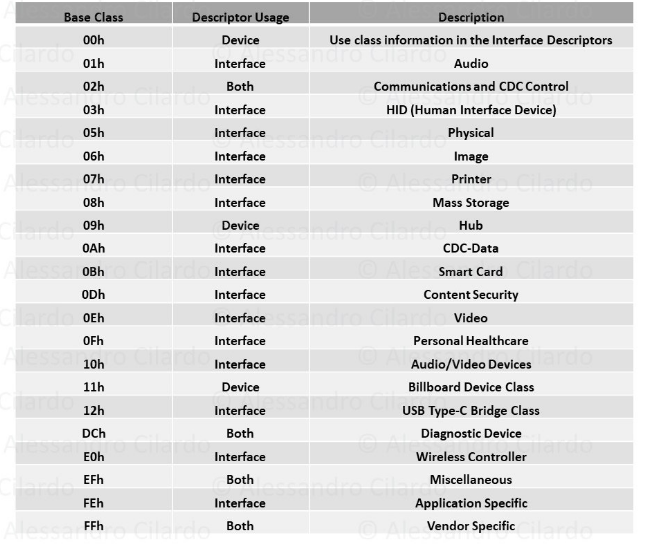
\includegraphics[width=.65\textwidth]{figures/ch1/protocols/usb-common-classes.png}
  \end{center}
  \caption{Classi comuni di dispositivi USB}\label{fig:usb-common-classes}
\end{figure}

L'architettura USB prevede diverse strutture logiche appartenenti anche allo stesso dispositivo dette \textbf{\textit{endpoint}} (\cref{fig:usb-endpoint-driver}). Ogni endpoint rappresenta una sorgente o una destinazione di dati (di fatto un buffer). Ogni dispositivo deve almeno specificare un endpoint di controllo. Gli endpoint di controllo sono bidirezionali, gli altri unidirezionali. Un altro concetto introdotto da USB sono le \textbf{\textit{pipe}}. Una pipe è un'astrazione che indica il collegamento tra due \textit{endpoint}.

\begin{figure}[H]
  \begin{center}
    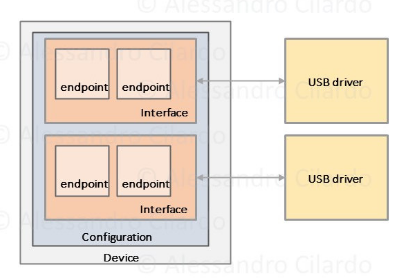
\includegraphics[width=.5\textwidth]{figures/ch1/protocols/usb-endpoint-driver.png}
  \end{center}
  \caption{Endpoint differenti nello stesso device}\label{fig:usb-endpoint-driver}
\end{figure}

USB definisce $4$ modalità di trasferimento:
\begin{itemize}
  \item Bulk: giusto per inviare grosse quantità di dati senza una certa cadenza.
  \item Isochronous: giusto per inviare di grosse moli di dati dati con tolleranza degli errori (audio/video);
  \item Control: invia pacchetti con requisiti di affidabilità e che quindi non possono essere persi;
  \item Interrupt: simile al control ma durante l'uso (tipo al mouse). Periodico non critico (ma critica l'integrità del pacchetto);
\end{itemize}

\subsubsection{ARM Microcontroller Bus Architecture: AMBA}
AMBA è un termine ombrello che indicano una famiglia di protocolli utilizzanti per le interconnessioni in ARM. Di questa famiglia, fanno parte AHB e APB indicati in \cref{fig:cortex-m4-arch}. Sono disponibili $5$ (\cref{fig:amba-evolution}) versioni di AMBA. 

\begin{figure}[h]
  \begin{center}
    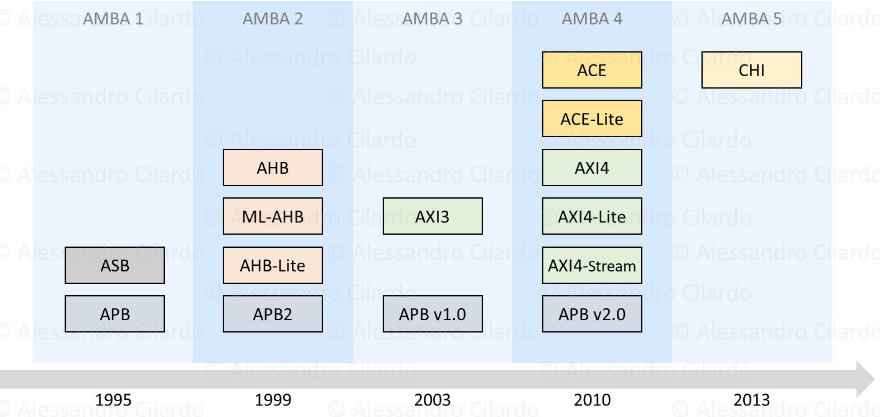
\includegraphics[width=.75\textwidth]{figures/ch1/protocols/amba-evolution.png}
  \end{center}
  \caption{Evoluzione delle suite di protocolli AMBA}\label{fig:amba-evolution}
\end{figure}

\paragraph{APB e AHB/ASB}
Nell prime versioni di AMBA ($1$ e $2$), i protocolli introdotti sono APB e AHB. L'\textbf{Advanced Peripheral Bus (APB)} viene usato per connettere periferiche \textit{low bandwidth} con un \textit{bus} condiviso e supporta più master e più slave, ma non supporta trasferimenti in \textbf{burst}. Si tratta di un protocollo semplice in cui i segnali di lettura e scrittura condividono gli stessi fili e viene utilizzato da periferiche semplici come \textbf{I2C}, \textbf{SPI} ecc. L'architettura tipica è mostrata in \cref{fig:ahb-apb-architecture} in cui si introduce un componente che fa adattattore tra APB e AHB.

\begin{figure}
  \begin{center}
    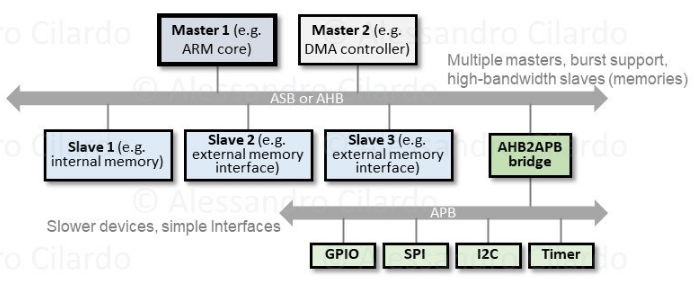
\includegraphics[width=.6\textwidth]{figures/ch1/protocols/ahb-apb-architecture.png}
  \end{center}
  \caption{Architettura con bus ad alte \textit{performance} insieme a periferiche semplici collegate con APB}\label{fig:ahb-apb-architecture}
\end{figure}

L'\textbf{Advanced High performance Bus (AHB)} sostituisce il vecchio \textbf{Advances System Bus (ASB)} e viene pensato per connettere quei dispositivi \textit{high bandwidth} come DMA, DSP su un bus condiviso. Supporta i trasferimenti in \textbf{burst}, ma essendo un protocollo con più master e più slave è un po' limitato dai sistemi di arbitraggio e indirizzamento (\cref{fig:ahb-architecture-detail}).

\begin{figure}
  \begin{center}
    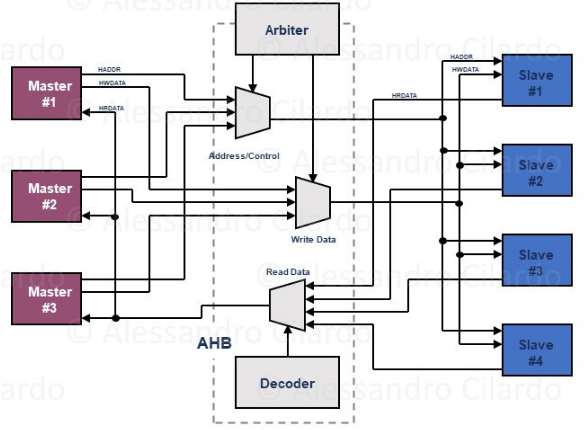
\includegraphics[width=.5\textwidth]{figures/ch1/protocols/ahb-architecture-detail.png}
  \end{center}
  \caption{Architettura interna di AHB}\label{fig:ahb-architecture-detail}
\end{figure}

\paragraph{Advanced Extensible Interface: AXI}
A partire dalla versione $3$ e $4$ di AMBA, viene introdotto AXI: un protocollo ottimizzato per le connessioni a banda larga e bassa latenza. Si tratta di una versione migliorata di AHB in cui vengono superati i limiti di un bus condiviso passando ad un interconnessione \textit{punto-punto}. L'interconnessione può essere uno switch o una rete dedicata \textit{on-chip} (\cref{fig:axi-connection}).

Andando nel dettaglio, AXI separa la parte di trasferimento dati da quello di controllo e fornisce un meccanismo per supportare transazioni \textit{outstanding}: è possibile iniziare nuove operazioni di lettura e scrittura con uno \textit{slave} anche non se quelle precedenti non sono completate (si può fare attraverso identificativi univoci ARID e AWID). Inoltre, sono supportate transazioni \textit{out-of-order}.

\begin{figure}[H]
  \begin{center}
    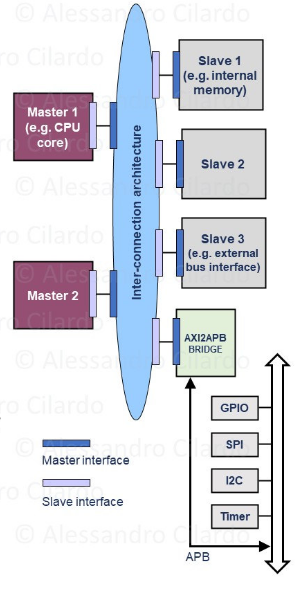
\includegraphics[width=.3\textwidth]{figures/ch1/protocols/axi-connection.png}
  \end{center}
  \caption{Schema di una connessione AXI}\label{fig:axi-connection}
\end{figure}

Il protocollo AXI supporta diverse modalità di trasferimento. Queste sono supportate dalla versione AXI-Full che ha tutte le caratteristiche. Esistono tuttavia altre due versioni del protocollo AXI: \textbf{\textit{AXI-Lite}} (che non supporta trasferimenti in \textit{burst}) e \textbf{\textit{AXI-Stream}}. Quest'ultimo aggiunge alcuni vincoli per massimizzare le performance in \textit{streaming}. Ad esempio, le trasmissioni diventano unidirezionali, non ci sono più canali separati per letture/scritture (\cref{tab:axi-modes}). Un confronto tra AXI-Full e AXI Stream è mostrato in \cref{tab:axi-full-vs-stream}.

In AMBA $4$ è stato esteso AXI con \textbf{AXI Coherence Extension (ACE)} che viene utilizzato da SoC con più core che devono implementare la coerenza nelle cache. Sostanzialmente, si aggiungono dei canali extra al classico AXI che servono ad implementare un protocollo \textbf{snoop based}. Anche questo protocollo ha una versione \textbf{Lite} in cui si implementa una coerenza in componenti che non hanno una cache, ma devono operare in un ambiente in cui è necessaria la coerenza come DMA o interfacce di rete. In AMBA $5$, è stato introdotto \textbf{Coherent Hub Interface (CHI)} basato su un protocollo a pacchetti a più livelli e supera alcune limitazioni di ACE e serve a gestire meglio integrazioni con diversi tipi di componenti: FPGA, GPU, DSP.

\begin{table}[h!]
\centering
\begin{tabular}{|l|c|c|l|}
\hline
\textbf{Modalità} & \textbf{Supporto Burst} & \textbf{Canali Indipendenti} & \textbf{Applicazioni Principali} \\ \hline
AXI Full          & Sì                      & Sì                           & Sistemi complessi con requisiti di alta velocità       \\ \hline
AXI-Lite          & No                      & Sì                           & Accesso a periferiche semplici e registri di controllo \\ \hline
AXI-Stream        & No (solo dati)          & Sì                           & Streaming dati continuo, video/audio, DSP              \\ \hline
\end{tabular}
\caption{Modalità di trasferimento supportate da AXI in AMBA 4}
\label{tab:axi-modes}
\end{table}

Inoltre in AXI, sono presenti $3$ tipi di burst (le principali differenze sono in \cref{tab:burst_types}):
\begin{itemize}
  \item \textbf{\textit{wrap}}: l'indirizzo di destinazione viene aggiorna in base ad un buffer circolare;
  \item \textbf{\textit{non incrementing (o fixed)}}: l'indirizzo di destinazione non cambia. Questo tipo di burst viene utilizzato per ricevere dati da un dispositivo seriale che hanno un porta assegnata
  \item \textbf{\textit{incrementing}}: trasferimento in cui l'indirizzo di destinazione viene incrementato (ARSIZE/AWSIZE). Viene utilizzato per dispositivi di memoria;
\end{itemize}

\begin{table}[h]
\centering
\begin{tabular}{|p{3cm}|p{7cm}|p{5cm}|}
\hline
\textbf{Tipo di Burst} & \textbf{Descrizione}                                                                                                                                 & \textbf{Applicazioni Tipiche}                                 \\ \hline
Fixed                  & L'indirizzo rimane costante per ogni trasferimento, i dati vengono scritti o letti dallo stesso indirizzo.                                           & Accesso a registri o periferiche con indirizzi statici.       \\ \hline
Incremental            & L'indirizzo si incrementa di una quantità pari alla dimensione dei dati per ogni trasferimento nel burst.                                           & Lettura/scrittura sequenziale in memoria, ad esempio in DRAM. \\ \hline
Wrapping               & Simile al burst incrementale, ma l'indirizzo si “avvolge” (ritorna indietro) se raggiunge un limite specificato (allineato alla lunghezza del burst). & Accesso a strutture dati circolari, ad esempio buffer circolari. \\ \hline
\end{tabular}
\caption{Confronto tra i tipi di burst supportati da AXI}
\label{tab:burst_types}
\end{table}


Dal punto di vista tecnico, AXI definisce $5$ canali. 
\begin{itemize}
  \item Address channels (AR, AW): sono due canali (separati per letture  e scritture) che forniscono tutt el informazioni di cotnrollo per le transazioni. In particolare, controllano il numero di trasferimenti per burst (da $1$ a $16$), la dimensione del trasferimento (fino a $1024$ bit) e il tipo di burst.
  \item Write Data Channel (W): formato da un bus dati ($8-1024$ bit) e un byte per inviare \textbf{strobe} \cref{fig:axi-write-channels};
  \item Read Data Channel (R): contiene un bus dati analogo al Write Data Channel e un bus in cui si ha una risposta che indica il completamento di un'operazione di lettura \cref{fig:axi-read-channels};
  \item Write Response Channel (B): serve ad uno slave ad inviare un segnale di completamento alla fine di ogni burst.
\end{itemize}

Ogni canale è indipendente dagli altri e contiene una propria coppia di segnali \textit{xVALID/xREADY}. Questi due segnali servono ad effettuare l'handshake per il trasferimento dati. In particolare, \textit{xVALID}, controllato dalla sorgente, informa la destinazione che i dati sono validi e possono essere letti; \textit{xREADY} viene utilizzato dal ricevente per notificare che è pronto a ricevere dati. Quando \textit{xREADY} e \textit{xVALID} sono entrambi alti si dice che è stato inviato un \textit{beat}.

\begin{figure}
\centering
\begin{subfigure}{.5\textwidth}
  \centering
  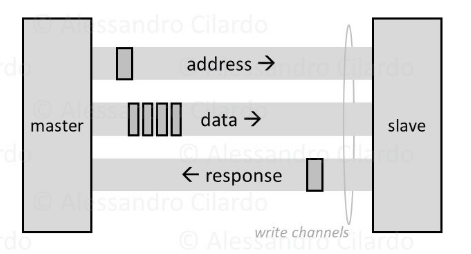
\includegraphics[width=.9\linewidth]{figures/ch1/protocols/axi-write-channels.png}
  \caption{Write Channels}
  \label{fig:axi-write-channels}
\end{subfigure}%
\begin{subfigure}{.5\textwidth}
  \centering
  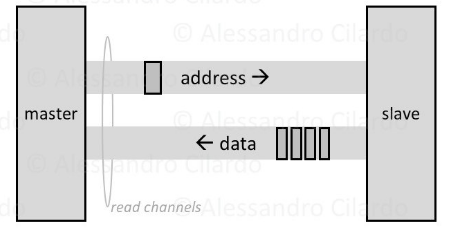
\includegraphics[width=.9\linewidth]{figures/ch1/protocols/axi-read-channels.png}
  \caption{Read Channels}
  \label{fig:axi-read-channels}
\end{subfigure}
\caption{AXI interazione base}

\end{figure}

Ci sono degli overhead rispetto ad AXI Full e AXI Stream che consentono di trasferire blocchi di dati più semplicemente. Ad esempio, si vuole inviare $1 KB$ di dati con un bus a $32-bi$ con AXI Full:
\begin{itemize}
  \item Ci sono $2-3$ cicli per inviare indirizzo e comandi;
  \item $1024/4 = 256$ trasferimenti;
  \item Ogni $16$ trasferimenti bisogna iniziare un nuovo burst in cui ci sono altri comandi;
  \item Dopo ogni trasferimento c'è una risposta da attendere;
\end{itemize}
Facendo lo stesso esercizio con AXI stream:
\begin{itemize}
  \item I dati vengono trasmessi in maniera diretta senza indirizzi;
\end{itemize}

\begin{table}[h!]
\centering
\renewcommand{\arraystretch}{1.2} % Aumenta lo spazio tra le righe
\begin{tabular}{|l|p{5cm}|p{5cm}|}
\hline
\textbf{Caratteristica} & \textbf{AXI Full} & \textbf{AXI Stream} \\ \hline
\textbf{Struttura del trasferimento} & 
Basato su indirizzi e dati. & 
Solo trasferimento di dati. \\ \hline
\textbf{Utilizzo del bus} & 
Multipli canali: indirizzo, dati, risposte. & 
Canale dati unidirezionale. \\ \hline
\textbf{Indirizzamento} & 
Supporta lettura e scrittura con indirizzi. & 
Nessun indirizzo: dati inviati in streaming. \\ \hline
\textbf{Tipi di burst} & 
Fixed, Incremental, Wrapping. & 
Non applicabile. \\ \hline
\textbf{Applicazioni tipiche} & 
Accesso a memoria, registri e periferiche. & 
Streaming dati, elaborazione video/audio, DSP. \\ \hline
\textbf{Coerenza} & 
Supporta ordini out-of-order tramite identificatori (ID). & 
Non necessario (stream continuo). \\ \hline
\textbf{Flusso dati} & 
Bidirezionale (lettura e scrittura). & 
Unidirezionale (master verso slave). \\ \hline
\textbf{Overhead} & 
Maggiore, a causa della gestione di indirizzi e risposte. & 
Minore, grazie all'assenza di indirizzi e risposte. \\ \hline
\textbf{Efficienza} & 
Ideale per accessi random e strutturati. & 
Altamente efficiente per trasferimenti continui e a basso overhead. \\ \hline
\end{tabular}
\caption{Confronto tra AXI Full e AXI Stream}
\label{tab:axi-full-vs-stream}
\end{table}

Un esempio di transazione di lettura è mostrato in \cref{fig:axi-read-transaction}. L'\textit{initiator} inizia una richiesta di lettura posizionando su \textit{ARADDR} l'indirizzo da cui partire a leggere ($0x0$), su \textit{ARSIZE} la dimensione di ciascun blocco da leggere ($4 bytes$), su \textit{ARLEN} quanti blocchi leggere ($3 + 1 = 4$) e su \textit{ARBURST} il tipo di burst (\textit{INCR}). Il ricevitore, dopo aver ricevuto \textit{ARVALID/ARREADY}, posiziona su \textit{RDATA} il risultato della lettura. In particolare, per l'indirizzo $0x0$ ritorna il valore $0x10$, per $0x4$ ritorna $0x11$, per $0x8$ ritorna $0x12$ e per $0xC$ ritorna $0x13$, tutti con codice \textit{OK}. All'ultima lettura alza il flag \textit{ARLAST}.

\begin{figure}
  \begin{center}
    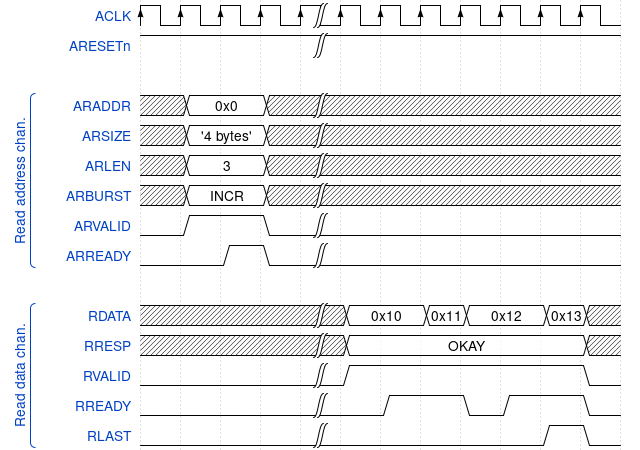
\includegraphics[width=.75\textwidth]{figures/ch1/protocols/axi-read-transaction.png}
  \end{center}
  \caption{Esempio di lettura in AXI}\label{fig:axi-read-transaction}
\end{figure}

Un esempio di transazione di scrittura è mostrato in \cref{fig:axi-write-transaction}.L'\textit{initiator} inizia una richiesta di scrittura posizionando su \textit{AWADDR} l'indirizzo da cui partire a scrivere ($0x0$), su \textit{AWSIZE} la dimensione di ciascun blocco da scrivere ($4 bytes$), su \textit{AWLEN} quanti blocchi scrivere ($3 + 1 = 4$) e su \textit{AWBURST} il tipo di burst (\textit{INCR}). Il ricevitore, dopo aver inviato \textit{AWVALID/AWREADY}, posiziona su \textit{WDATA} i dati da scrivere asserendo \textit{WVALID} e \textit{WLAST} per l'ultimo blocco. Il target ritorna un \textit{BRESP} dopo tutta la transazione. 

\begin{figure}[H]
  \begin{center}
    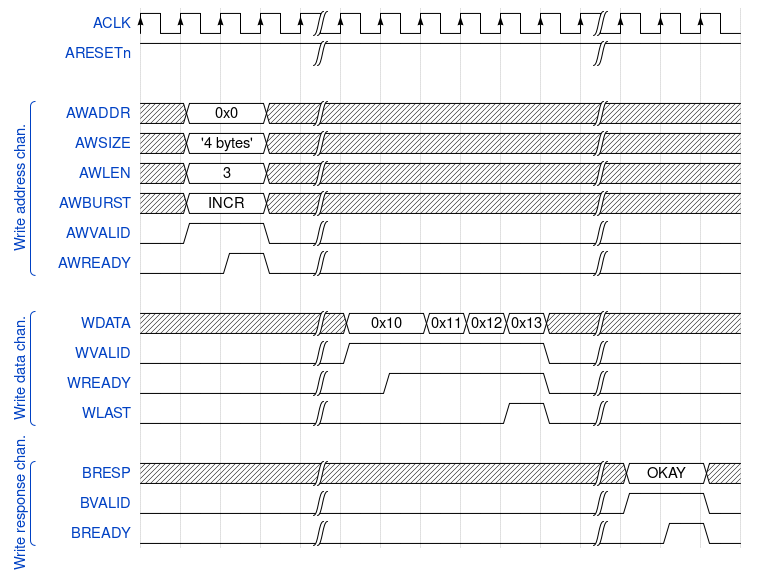
\includegraphics[width=.75\textwidth]{figures/ch1/protocols/axi-write-transaction.png}
  \end{center}
  \caption{Esempio di scrittura in AXI}\label{fig:axi-write-transaction}
\end{figure}

\clearpage
\subsection{MPSoC: Cortex A e FPGA}
In questa sezione, si studiano le caratteristiche principali di un MPSoC ARM con un FPGA integrato. Tutte le terminologie utilizzate sono proprie del gergo Xilinx che ha progettato questa integrazione. Alcuni esempi, faranno riferimento alla Zynq-7000 (dotato di un dual core Cortex-A9) e alla Zynq Ultrascale+ (con quad-core Cortex-A, GPU e RPU \cref{fig:zynq-ultrascale}). La prima distinzione che si effettua sull'MPSoC è tra \textbf{\textit{PS} (Processing system)} (riferita alla parte ARM) \textbf{\textit{PL} (Programmable Logic)}.

\begin{figure}[h]
  \begin{center}
    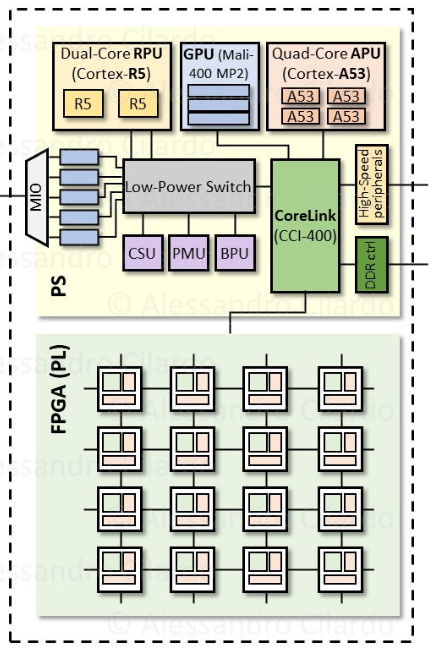
\includegraphics[width=.5\textwidth]{figures/ch1/mpsoc/zynq-ultrascale.png}
  \end{center}
  \caption{Architettura di un MPSoC dotato sia di parte PL che PS}\label{fig:zynq-ultrascale}
\end{figure}

\subsubsection{SoC: Zynq 7000}
Si tratta di un SoC dotato di $2$ core Cortex-A9 (basato su ARMv7) che può eseguire un sistema operativo completo come Linux. I dettagli sono mostrati in \cref{fig:zynq-7000-soc-detail}. L'idea di questi sistemi è quella di demandare logica custom alla parte PL scrivendo eventualemente anche delle routine in C per gestire la comunicazione con protocolli complicati. Il SoC predispone un'architettura con bus AMBA per la gestione delle comunicazioni con periferiche standard tra cui anche un modulo di memoria DDR3 da 1GB. 

\begin{figure}[h]
  \begin{center}
    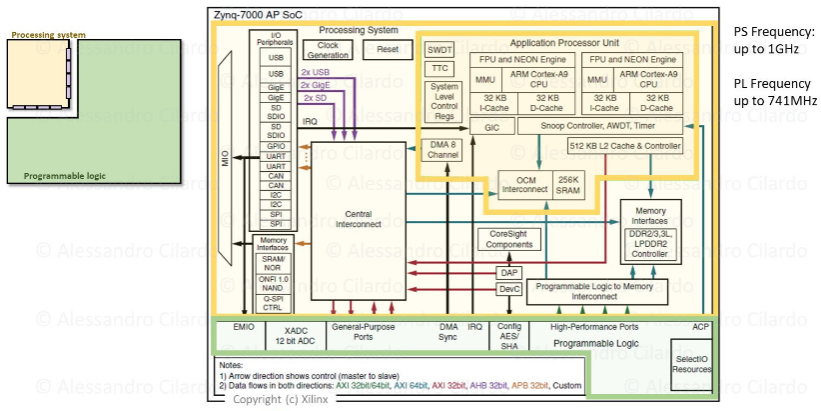
\includegraphics[width=.85\textwidth]{figures/ch1/mpsoc/zynq-7000-soc-detail.png}
  \end{center}
  \caption{Dettaglio della Zynq-7000}\label{fig:zynq-7000-soc-detail}
\end{figure}

La parte PS può essere divisa in due regioni (\cref{fig:zynq-7000-soc-detail}): la prima è detta \textbf{\textit{APU} (Application Processor Unit)}, l'altra è dedicata alle interconnessioni e contiene i controller per l'I/O gestiti con MIO (\textbf{\textit{multiplexted input/output}} i pin possono essere configurati per avere una periferica piuttosto che un'altra), i componenti di memoria e l'interfacciamento con la parte PL. Nell'APU, sono presenti due core A9 con l'estensione vettoriale NEON. I due core condividono un livello di \textit{cache L2} e la \textbf{\textit{Snoop Control Unit} (SCU)} che supporta un protocollo di coerenza a $3$ stati (\textit{modify, share, embed}) e hanno una cache \textit{L1} interna divisa tra dati ed istruzioni. 

\paragraph{Interruzioni}
Come mostrato in \cref{fig:interrupts-gic-detail}, le interruzioni devono non solo essere controllate dalla parte ARM, ma anche da quella PL e sono indicate con \textbf{\textit{shared interrupt}} (possono essere dirottate ovunque. Tutte le periferiche esterne, i controller di memoria, ricadono in questa categoria. In realtà i loro segnali di interruzione possono essere anche inoltrati verso la parte FPGA, quindi, c'è un multiplexer (sempre dove sta la freccia rossa) che può essere configurato insieme a molte altre cose in questa parte PS e permette di far arrivare certi segnali di interruzione nella parte FPGA; questo vuol dire che è possibile sviluppare dei componenti che reagiscono a un'interruzione sollevata da un controller USB nella parte PS. Alcuni gruppi di segnali come timer, watchdog sono detti \textbf{\textit{Private Peripherals Interrupts}} e sono private ai core insieme alle cosiddette \textbf{\textit{Software Generated Interrupts} (SGI)}. La parte generica è gestita da un GIC PL390 che distingue una parte di IRQ/FIQ per ciascun core.
\begin{figure}[H]
  \begin{center}
    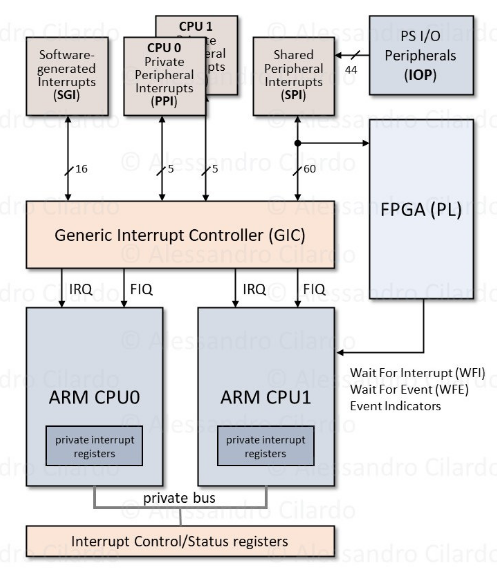
\includegraphics[width=.5\textwidth]{figures/ch1/mpsoc/interrupts-gic-detail.png}
  \end{center}
  \caption{Gestione delle interruzioni}\label{fig:interrupts-gic-detail}
\end{figure}

Tutto questo si complica se si tiene conto del fatto che la parte FPGA deve essere anche essa sorgente di interruzioni e che queste devono avere una certa priorità. Un sistema   più dettagliato è mostrato in \cref{fig:interrupt-management}.

\begin{figure}[H]
  \begin{center}
    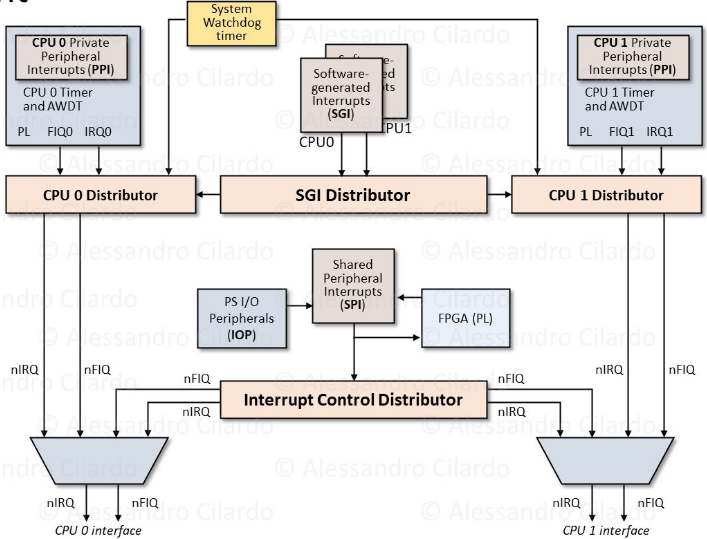
\includegraphics[width=.65\textwidth]{figures/ch1/mpsoc/interrupt-management.png}
  \end{center}
  \caption{Gestione delle interruzioni nel dettaglio}\label{fig:interrupt-management}
\end{figure}

\paragraph{Programmable logic} La programmable logic è un FPGA a tutti gli effetti e quindi contiene celle riconfigurabili. Nel corso degli anni gli FPGA Xilinx sono stati voluti per supportare funzionalità anche mediamente complesse ricorrenti nella pratica, ad esempio per fare calcolo in algoritmi orientati a DSP (Digital Signal Processing) dove fondamentalmente il pattern ricorrente di base è il multiply-accumulate, quindi la coppia moltiplicazione seguita dall'accumulazione in un registro abbastanza grande da contenere una somma di prodotti parziali (quello che faccio ad esempio in un filtro FIR) e per questo praticamente tutti gli FPGA offrono anche dei componenti che si chiamano dedicated DSP block che hanno all'interno dei moltiplicatori, non sono in logica riconfigurabile ma sono fatti direttamente su Silicio e sono dislocati in punti distribuiti dell'FPGA. Un altro componente fondamentale sugli FPGA è costituito da quelli che si chiamano \textbf{\textit{BlockRAM}}, piccoli blocchi di memoria dell'ordine dei $18-36 kB$ (pensati di essere usati a banchi di $9$ bit per includere un bit di parità).

Il mondo PL e PS comunicano o attraverso AXI o con \textbf{\textit{Extended Multiplexed Input/Output (EMIO)}} (per la comunicazione con periferiche dedicate). Tutto questo è integrato nel flusso di sviluppo: creando un moltiplicatore è possibile chiedere che gli ingressi $a$ e $b$ provengano da un'interfaccia AXI Stream per avere il massimo throughput. In \cref{fig:ps-pl-interfaces}, è mostrata in dettaglio la comunicazione. In particolare, sono previsti $3$ tipi di interfacce tra PL e PS:
\begin{itemize}
  \item High performance ports: strutture FIFO per la comunicazione burst a $32-64bit$;
  \item Accelerator Coherence Port: serve a far comunicare la PL con SCU all'interno dell'APU per la coerenza tra le cache.
  \item General Purpose AXI: avere ad una comunicazione a $32-bit$. La parte PS si compora da master;
\end{itemize}

\begin{figure}
  \begin{center}
    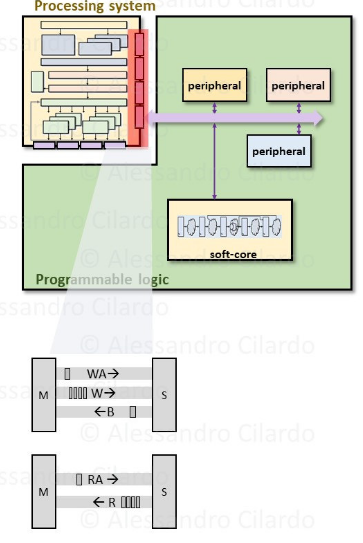
\includegraphics[width=.4\textwidth]{figures/ch1/mpsoc/ps-pl-interfaces.png}
  \end{center}
  \caption{Interfacce tra Processing System e Programmable Logic}\label{fig:ps-pl-interfaces}
\end{figure}

\subsubsection{Zynq Ultrascale+}
La Zynq-Ultrascale è la controparte più potente della Zynq-7000 dotata di un processore di fascia medio alta. In particolare, può avere fino a $4$ core di un Cortex-A53 che è basato su architettura ARMv8. La sua struttura conserva la ripartizione in PS e PL ed è illustrata in \cref{fig:zynq-ultrascale-arch}. Un caso d'uso potrebbe essere effettuare codifica/decodifica di stream video utilizzando la parte PL e poi sfruttare la GPU Mali per fare rendering. 

Come mostrato in \cref{fig:zynq-ultrascale-variants}, la Ultrascale è una famiglia di schede leggermente configurabile: ad esempio, si può decidere il numero di core del Cortex-A, se includere o meno una GPU e se aggiungere delle RPU (basate sul Cortex-R5) dotati di \textbf{\textit{Tight Coupled Memory} (TCM)} utili per elaboraziioni \textbf{\textit{real-time}}. Inoltre, a che la parte PL può essere dimensionata e in realtà, si possono trovare anche dei componenti su silicio che servono ad applicazioni specifiche: i \textbf{\textit{macro-core}}. I \textit{macro-core} sono dei blocchi hardware che supportano codec (come H264 e H265) e altre funzionalità tipiche del blocco DSP e non sono configurabili, ma cablati.

\begin{figure}
  \begin{center}
    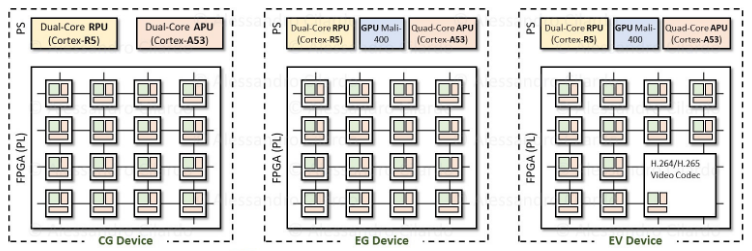
\includegraphics[width=0.95\textwidth]{figures/ch1/mpsoc/zynq-ultrascale-variants.png}
  \end{center}
  \caption{Varianti della Zynq ultrascale}\label{fig:zynq-ultrascale-variants}
\end{figure}

\paragraph{Interruzioni} Essendo basata su ARMv8, le interruzioni possono essere complicate leggeremente per supportare i \textit{guest} con l'introduzione di \textbf{\textit{virtual interrupt}}. I livelli distributor del GIC-400 (\cref{fig:zynq-ultrascale-gic}) sono analoghi a quelli della Zynq e sono privati ai core fisici. AL secondo livello, è possibile specificare una vCPU attraverso un blocco hardware messo a disposizione dal GIC e sono destinate alle macchine virtuali.

\begin{figure}[h]
  \begin{center}
    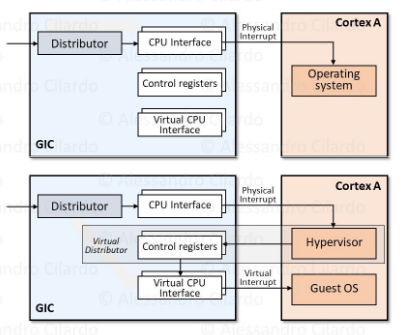
\includegraphics[width=.5\textwidth]{figures/ch1/mpsoc/zynq-ultrascale-gic.png}
  \end{center}
  \caption{Struttura GIC in ARMv8}\label{fig:zynq-ultrascale-gic}
\end{figure}

\paragraph{GPU Mali}
La GPU utilizzata dalla Ultrascale è una Mali-400 MP2 (\cref{fig:zynq-ultrascale-mali}). Non si tratta di una GPU di tipo GP (General Purpose), quindi su questa GPU non è possibile programmare con CUDA, né con OPENCL. Si tratta piuttosto di un acceleratore grafico, quindi presenta, cablato nella sua struttura, la pipe
grafica con 2 macro componenti:
\begin{itemize}
  \item Geometry processor;
  \item Pixel Processor;
\end{itemize}
Questi componenti lavorano fondamentalmente in maniera hardware o firmware su quelli che sono gli step fondamentali della pipeline grafica, che permette di passare da un modello “vettoriale” della scena al \textbf{\textit{rendering raster}} (bitmap).  I vari Processor hanno un accesso alla gerarchia di memoria e hanno una loro MMU, dunque l’interfacciamento al resto del sistema è simile a quello dell’ RPU e dell’APU. Quello che rende più o meno standard l’integrazione di questi acceleratori non è la programmabilità in software ma è un API che si chiama \textit{OPENGL} nel profilo \textbf{\textit{ES (Embedded System)}}, la quale è un API per primitive di calcolo grafico relativamente di basso livello ed è quella che molte GPU anche in ambito mobile supportano.

\begin{figure}
  \begin{center}
    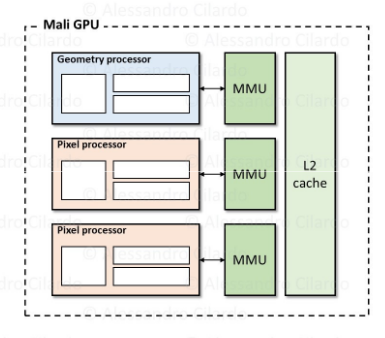
\includegraphics[width=.5\textwidth]{figures/ch1/mpsoc/zynq-ultrascale-mali.png}
  \end{center}
  \caption{Architettura di una GPU Mali}\label{fig:zynq-ultrascale-mali}
\end{figure}

\paragraph{Periferiche}
La UltraScale è un dispositivo molto complesso nel quale coesistono molte parti, non tutte necessarie in una determinata applicazione, per cui viene prevista la possibilità di accendere o spegnere
selettivamente alcune di queste parti, tra cui anche lo stesso FPGA e questo viene fatto attraverso il meccanismo dei \textbf{domini di potenza} gestito da un componente detto \textbf{\textit{Power Mode Unit} (PMU)}. Esistono 4 diversi modi di utilizzo:
\begin{itemize}
  \item \textbf{\textit{Full-Power Domain}}: la scheda utilizza tutti gli accelatori, processori e periferiche;
  \item \textbf{\textit{Idle}}: in cui si tiene accesa la RAM e consente al sistema di restare vivo prima di essere spento;
\end{itemize}

Per quanto riguarda le periferiche presenti, le \textbf{\textit{Low Speed Peripherals}} sono quelle già viste come CAN, GPIO, UART ecc. Poi ci sono quelle più esigenti, dette \textbf{\textit{High Speed Peripherals}} come USB 3.0 che ha un ordine di grande in più di throughput rispetto a USB 2.0, poi SATA, GigE (gigabit ethernet). Si tratta di interfacce che richiedono bande non gestibili tramite pin general purpose e sono gestite fisicamente in modo diversIl pezzo di High Speed è direttamente accoppiato alla parte APU a differenza della parte RPU, la quale è invece immaginata per un utilizzo più disaccoppiato col processore. Il canale che collega la parte High Speed Peripherals e il processore deve essere in grado di sostenere una banda compatibile con quello che faccio con le varie interfacce (SATA, USB etc..) e lo stesso vale per i pin in uscita, che devono essere progettati fisicamente in maniera diversa. Quello che poi fisicamente esce verso l’esterno dalla parte High Speed dipende da quali periferiche sono effettivamente presenti. 

Inoltre, questo sistema è un esempio di sistema nel quale interviene la \textbf{\textit{SMMU (System MMU}} che è la controparte della MMU attaccata ai processori e permette di supportare la traduzione degli indirizzi a 2 livelli in sistemi che abbiano virtualizzazione. Questo è un problema che troviamo in diversi contesti; nei processori \textit{x86} Intel/AMD, si trova lo stesso tipo di problematica cioè il supporto sia lato CPU sia lato dispostivi; nel caso di Intel si parla di I/O MMU che è la controparte di questa SMMU, ed ha lo stesso scopo cioè mediare tra lo spazio di indirizzi visto dall’applicazione e lo spazio di indirizzi fisico, tenendo presente che ci può essere un livello intermedio nel quale quello che è l’indirizzo fisico per un layer che è una macchina virtuale, in realtà è a sua volta un indirizzo virtuale e che deve quindi essere tradotto. Questa MMU è piazzata immediatamente al di fuori della parte APU tra le periferiche e la memoria fisica vera e propria e può essere configurata dal software di gestione in modo da allineare la traduzione degli indirizzi fatta lato APU con la traduzione degli indirizzi vista dai dispositivi; quello che ci consente di fare, ad esempio, un DMA tra indirizzi virtuali “guest” (cioè visti dalla macchina virtuale), chiedendo ad un Controller DMA, che è all’esterno del aprocessore e quindi esterno al meccanismo di traduzione degli indirizzi, di usare in maniera coerente i miei indirizzi virtuali.

\paragraph{Programmazione}
Le piattaform viste possono essere utilizzate sia con software \textit{bare-metal} che attraverso un \textit{runtime} quale un sistema operativo. La differenza sta sia nella granularità con cui si controlla la configurazione e può avere pro e contro. Ad esempio, la possibilità di usare un kernel in evoluzione può favorire sia la metrica del \textit{time to market} come quella della portabilità e riutilizzo del codice. Un sistema operativo usato su Cortex-A è il ben noto Android OS che ormai ha un architettura consolidata (\cref{fig:android-architecture}), basata sul kernel Linux. 

\begin{figure}
  \begin{center}
    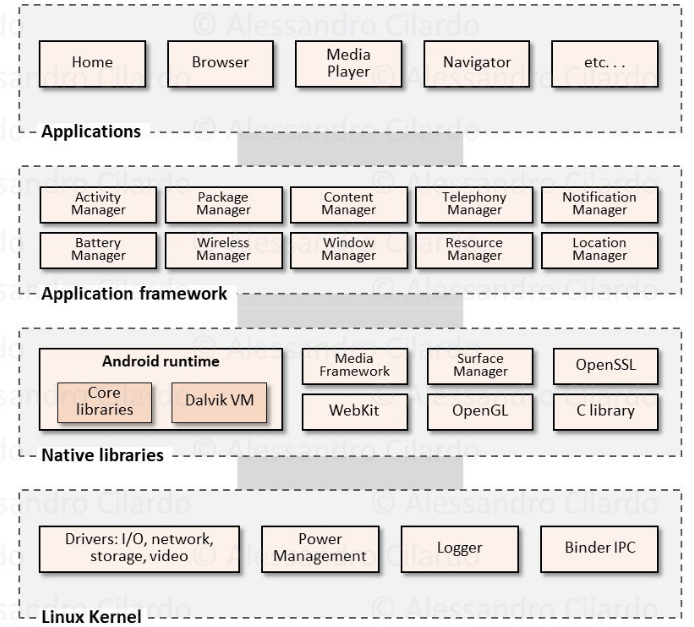
\includegraphics[width=.5\textwidth]{figures/ch1/mpsoc/android-architecture.png}
  \end{center}
  \caption{Architettura Android su processori Cortex-A}\label{fig:android-architecture}
\end{figure}


In generale, definita la piattaforma di base, vengono a crearsi diverse astrazioni (\cref{fig:abstraction}) che integrano i componenti previsti dal manufacturer. Ad esempio, il punto immediatamente dopo l'hardware è il \textbf{\textit{Board Support Package}} in cui si espongono funzionalità standard attraverso un API. Di recente, si sta cercando di introdurre il termine \textbf{\textit{Asymmetric Multi Processing}(AMP)}  in contrasto con il \textit{Symmetric Multi Processing} (SMP) in cui stack software diversi vengono eseguiti su hardware omogenei. Ad esempio un RTOS può girare insieme ad un GPOS. Infatti, Xilinx gestisce OpenAMP che mette a disposizione meccanismi di sincronizzazione e comunicazione per task che eseguono su hardware diversi ad esempio un RPU con un APU.

\begin{figure}
  \begin{center}
    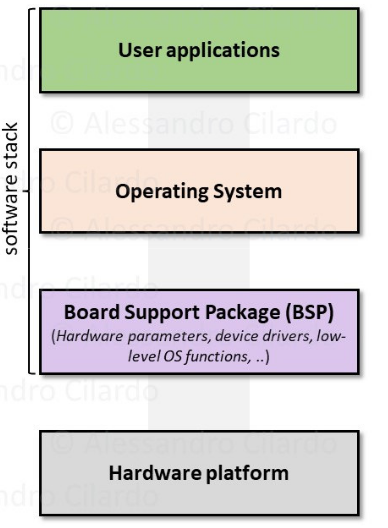
\includegraphics[width=.25\textwidth]{figures/ch1/mpsoc/abstraction.png}
  \end{center}
  \caption{Livelli di astrazione software dall'hardware}\label{fig:abstraction}
\end{figure}

\clearpage
\section{Strumenti ed esercitazioni}
\subsection{Toolchain GNU}
La toolchain GNU è un insieme di progetti che si occupano di coprire tutto il ciclo di sviluppo del software per le architetture più comuni inclusa ARM. Il flusso principale è mostrato in \cref{fig:gnu-software-dev-cycle}.
\begin{itemize}
  \item GCC: comunemente detto compilatore. In realtà, richiama tutti gli altri componenti;
  \item AS: assemblatore. Converte codice assembler in codice macchina;
  \item LD: linker. Collega tutti gli oggetti di compilazione;
  \item GDB: debugger;
  \item objcopy: impacchetta l'eseguibile come prodotto finale prendendo in ingresso l'uscita del linker
  \item objdump: effettua l'operazione di disassemlaggio;
\end{itemize}

\begin{figure}[h]
  \begin{center}
    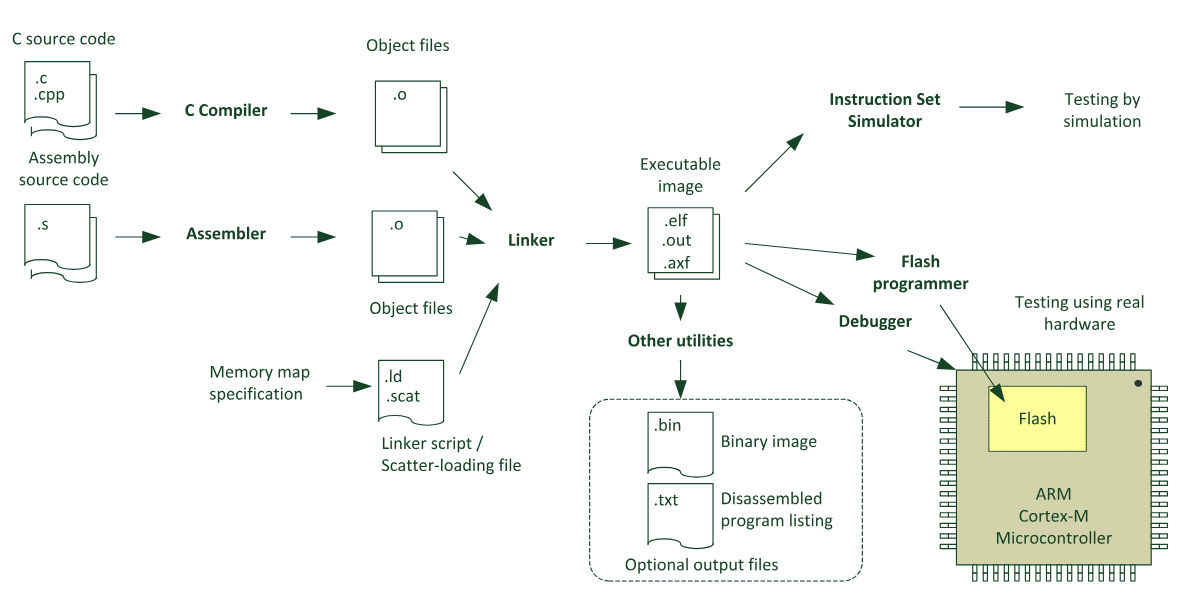
\includegraphics[width=0.95\textwidth]{./figures/ch2/software-development-cycle.png}
  \end{center}
  \caption{Ciclo di sviluppo con GNU toolchain}\label{fig:gnu-software-dev-cycle}
\end{figure}

Quando si usano le funzioni del C, si sta usando anche il suo runtime. Ad esempio, per allocare la memoria C mantiene delle sue strutture dati interne.

\subsubsection{Linkerscript}
Il \textbf{linkerscript} (detto anche \textbf{scatter-load}) è un file che prende in ingresso il Linker per capire come fare il layout in memoria del codice prodotto dalla compilazione. Un linkerscript minimale contiene:
\begin{itemize}
  \item entrypoint: punto da cui bisogna partire l'esecuzione. Una volta caricato il programma, il PC sarà impostato alla prima istruzione indicata dalla direttiva \textit{ENTRY};
  \item definizione della memoria (direttiva \textit{MEMORY}): può essere divisa in RAM, FLASH ecc. Per ciascun componente, bisogna specificare l'indirizzo di partenza e la dimensione;
  \item sezioni del codice (direttiva \textit{SECTIONS}): in base al tipo di eseguibile, si definiscono delle sezioni navigabili attraverso label. Ad esempio si configura la sezione \textit{text} in cui risiede il codice del programma da caricare, o quella del vettore delle interruzioni. Per ciascuna sezione si indica dove risiede (RAM o FLASH);
\end{itemize}

\lstinputlisting[caption="Linkerscript minimale",captionpos=bottom]{./code/base/linker_script.ld}

In generale, si parte da un programma scritto in $C$. Questo programma viene compilato in codice oggetto (utilizzando il flag \textit{-c}) ottenendo un \textbf{.o}. Al linkerscript di seguito, bisogna associare effettivamente del codice che corrisponde alla funzione \textbf{init} che si occupa di inizializzare la memoria con le indicazioni del linkerscript. Questo può essere fatto sia in assembler che in $C$. Ad esempio, in è mostrato un esempio minimale di setup. 

\lstinputlisting[language=C, caption="File di startup in C",captionpos=bottom]{./code/base/startup.c}

\subsection{Infrastruttura di debug}
\subsubsection{Semi-hosting}
\subsection{CMSIS}
\subsection{Introduzione a CMSIS}
Il \textbf{Cortex Microcontroller Software Interface Standard (CMSIS)} è un framework sviluppato da ARM per standardizzare l'accesso alle periferiche dei microcontrollori basati su Cortex-M. CMSIS fornisce un'interfaccia comune per l'accesso alle funzionalità del processore e delle periferiche, facilitando lo sviluppo di software portabile e riutilizzabile.

Uno degli elementi fondamentali di CMSIS è la funzione \textbf{SystemInit()}. Questa funzione viene chiamata all'inizio del programma, prima della funzione \textit{main()}, e si occupa di inizializzare il sistema. In particolare, \textit{SystemInit()} configura il clock del sistema, la memoria e altre periferiche essenziali. Ecco un esempio di come potrebbe apparire una funzione \textit{SystemInit()}:

\begin{lstlisting}[language=C]
void SystemInit(void) {
    // Configura il clock del sistema
    SystemClock_Config();
    
    // Configura la memoria
    Memory_Config();
    
    // Configura altre periferiche essenziali
    Peripheral_Config();
}
\end{lstlisting}

\subsection{Utilità di CMSIS}
CMSIS è utile per diverse ragioni:
\begin{itemize}
    \item \textbf{Portabilità}: Fornisce un'interfaccia standard che rende il codice portabile tra diversi microcontrollori basati su Cortex-M.
    \item \textbf{Efficienza}: Ottimizza l'accesso alle funzionalità del processore e delle periferiche, migliorando le prestazioni del sistema.
    \item \textbf{Semplicità}: Riduce la complessità dello sviluppo software fornendo un'API semplice e coerente.
\end{itemize}

\subsection{HAL e Gestione da parte di STM}
La \textbf{Hardware Abstraction Layer (HAL)} è una parte importante di CMSIS che fornisce un'interfaccia di alto livello per l'accesso alle periferiche hardware. STM (STMicroelectronics) ha esteso CMSIS con la propria libreria HAL, che include driver per tutte le periferiche dei microcontrollori STM32.

La libreria HAL di STM è organizzata in moduli, ciascuno dei quali gestisce una specifica periferica (ad esempio, GPIO, UART, SPI, ecc.). Ogni modulo include funzioni per configurare, inizializzare e utilizzare la periferica. Ecco un esempio di come potrebbe apparire l'uso della libreria HAL per configurare un GPIO:

\begin{lstlisting}[language=C]
#include "stm32f4xx_hal.h"

void GPIO_Config(void) {
    // Abilita il clock per il GPIO
    __HAL_RCC_GPIOA_CLK_ENABLE();
    
    // Configura il pin come output
    GPIO_InitTypeDef GPIO_InitStruct;
    GPIO_InitStruct.Pin = GPIO_PIN_5;
    GPIO_InitStruct.Mode = GPIO_MODE_OUTPUT_PP;
    GPIO_InitStruct.Pull = GPIO_NOPULL;
    GPIO_InitStruct.Speed = GPIO_SPEED_FREQ_LOW;
    HAL_GPIO_Init(GPIOA, &GPIO_InitStruct);
}

int main(void) {
    // Inizializza la libreria HAL
    HAL_Init();
    
    // Configura il sistema
    SystemInit();
    
    // Configura il GPIO
    GPIO_Config();
    
    // Ciclo principale
    while (1) {
        // Accende il LED
        HAL_GPIO_WritePin(GPIOA, GPIO_PIN_5, GPIO_PIN_SET);
        
        // Attende
        HAL_Delay(500);
        
        // Spegne il LED
        HAL_GPIO_WritePin(GPIOA, GPIO_PIN_5, GPIO_PIN_RESET);
        
        // Attende
        HAL_Delay(500);
    }
}
\end{lstlisting}

In questo esempio, la funzione \textit{GPIO\_Config()} utilizza la libreria HAL di STM per configurare un pin GPIO come output. La funzione \textit{main()} inizializza la libreria HAL, chiama \textit{SystemInit()} per configurare il sistema, e poi chiama \textit{GPIO\_Config()} per configurare il GPIO. Nel ciclo principale, il programma accende e spegne un LED collegato al pin GPIO.

\begin{figure}
  \begin{center}
    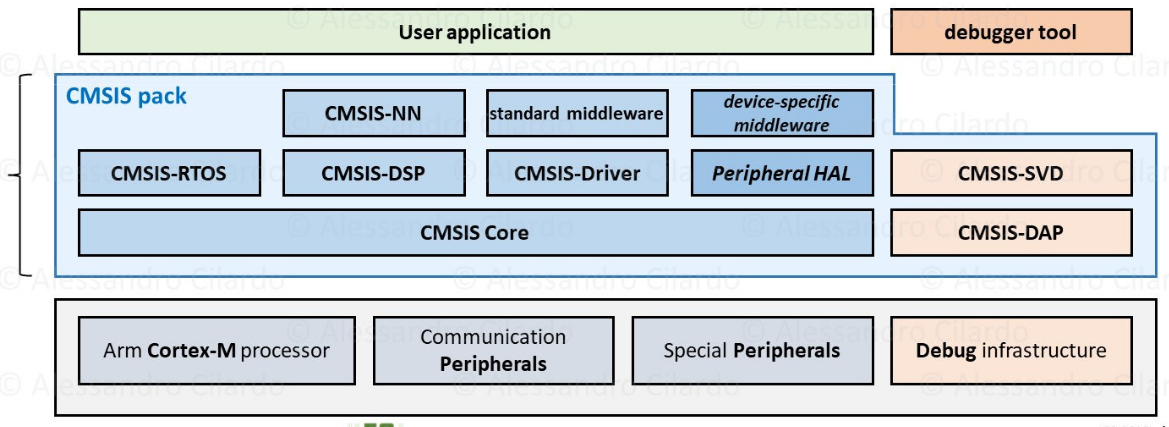
\includegraphics[width=.75\textwidth]{figures/ch2/cmsis.png}
  \end{center}
  \caption{Struttura di CMSIS}\label{fig:cmsis-structure}
\end{figure}

\subsection{FreeRTOS}
FreeRTOS è un sistema operativo real-time open source nel contesto embedded ed è supportato dalla maggior parte dei Cortex-M con supporto per il multitasking, l'\textit{inter process communication} con delle primitive di sincronizzazione, gestione di task (\cref{fig:freertos-task-state}) e \textbf{\textit{co-routine}} con un focus sulla predicibilità delle operazioni e sul ridotto \textit{footprint} (dai $4kb$ ai $9kb$). Funzionando su micro-controllori non ha supporto alla memoria virtuale e, pertanto, i processi hanno un proprio spazio di indirizzamento, ma utilizza la \textit{MPU} per isolare i \textit{task} utente da quelli \textit{real-time}. 

\begin{figure}[h]
  \begin{center}
    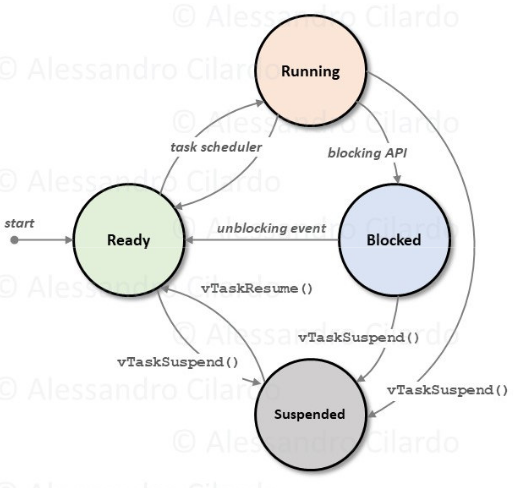
\includegraphics[width=.5\textwidth]{figures/ch2/freertos-task-state.png}
  \end{center}
  \caption{Stati di un task in FreeRTOS}\label{fig:freertos-task-state}
\end{figure}

Lo scheduler real-time è a priorità fissa, come mostrato in \cref{fig:freertos-scheduling}.
\begin{figure}
  \begin{center}
    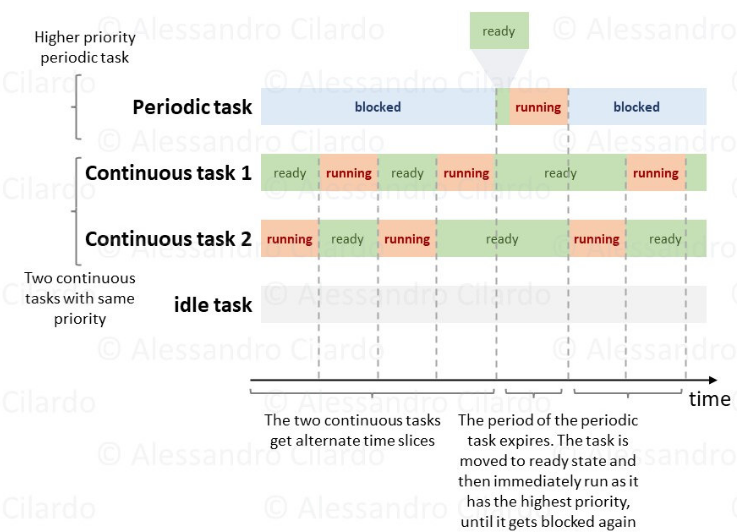
\includegraphics[width=.75\textwidth]{figures/ch2/freertos-scheduling.png}
  \end{center}
  \caption{Esempio di scheduling in FreeRTOS}\label{fig:freertos-scheduling}
\end{figure}

L'organizzazione è molto semplice in quanto la maggior parte del codice è concentrata in $4$ file:
\begin{itemize}
  \item \textit{Port.c}: modulo contenente tutto ciò che è dipendente dall’architettura target. Tutti gli accorgimenti che riguardano l’architettura, come la gestione del link register fatta da
ARM;
  \item \textit{List.c}: modulo per la gestione delle liste;
  \item \textit{Queue.c}: modulo per la gestione della comunicazione;
  \item \textit{Task.c}: modulo per la gestione dei Task;
\end{itemize}

Vi è inoltre una directory relativa alla parte di gestione della memoria, \textbf{MemMang}, che contiene differenti implementazioni di routine per la gestione della memoria dinamica. La gestione della memoria è un aspetto delicato in un RTOS poiché, nonostante la memoria dinamica consenta maggiori flessibilità alle applicazioni, pone problemi riguardanti il determinismo. Allocare un blocco di memoria significa trovare un blocco contiguo nell'area heap. Questa ricerca può essere onerosa poichè si tratta di un problema di \textit{bin packing} che può essere risolto con alcune euristiche come \textit{best fit}, \textit{worst fit} o \textit{first fit}. Inoltre, nelle implementazioni più avanzate può essere supportato l'utilizzo non continuo di memoria che aggiunge un ulteriore \textit{overhead} nell'utilizzo delle risorse. Un'altra fonte di indeterminismo riguarda la liberazione della memoria: bisogna aggiornare una struttura dati e fare il \textit{coalescing} dei blocchi di memoria continui.

FreeRTOS offre $5$ profili per gestire l'heap e sono implementati nei file $heap\_x.c$ in cui sostanzialmente sono offerte diverse versioni di \textbf{\textit{malloc()}} e \textbf{\textit{free()}}. All'aumentare del $x$ diminuisce il grado di predicibilità della gestione \textit{heap}. 
\begin{itemize}
  \item \textit{heap\_1.c}: non libera mai lo spazio, ma semplicemente mette il puntatore a $NULL$. 
  \item \textit{heap\_2.c}: libera l'heap, ma non effettua il coaelescing;
  \item \textit{heap\_3.c}: ingloba la malloc e la free del compilatore aggiungendo meccanismi di \textbf{\textit{thread safety}};
  \item \textit{heap\_4.c}: libera l'heap ed effettua il coaelescing per evitare la frammentazione della memoria. Esempio in \cref{fig:freertos-heap-4-example};
  \item \textit{heap\_5.c}: uguale al $4$, ma consente di allocare la memoria attraverso aree non adiacenti; 
\end{itemize}

\begin{figure}[H]
  \begin{center}
    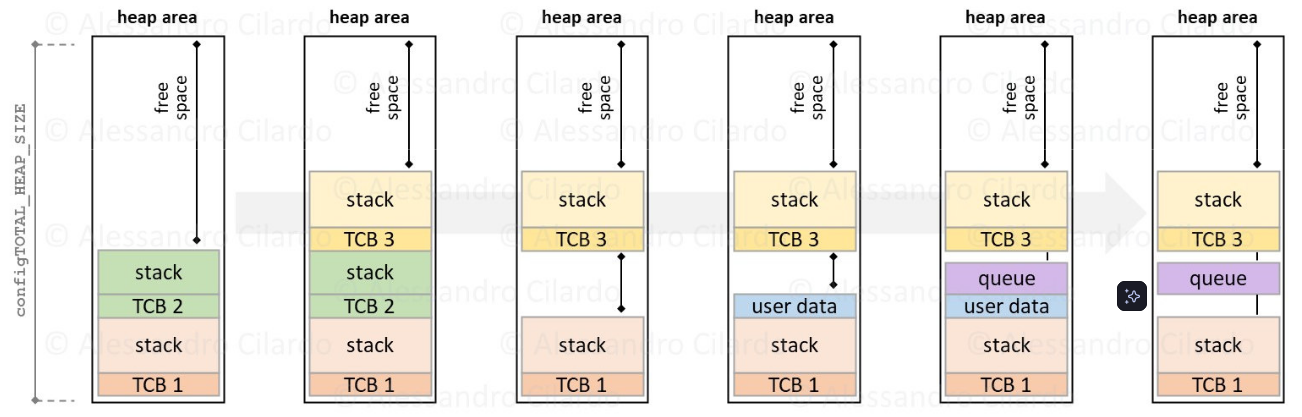
\includegraphics[width=0.95\textwidth]{figures/ch2/freertos-heap-4-example.png}
  \end{center}
  \caption{Esempio di funzionamento con la versione $4$ dell'heap}\label{fig:freertos-heap-4-example}
\end{figure}

\subsection{Linux}
Il kernel fornisce fondamentalmente funzionalità come gestione della \textit{virtual memory},  ciclo di vita dei processi, astrazione dei dispositivi con supporto per driver e anche framework costruiti \textit{on-top-of} dei driver, per esempio per esporre delle API portabili di alto livello rispetto ad una serie di funzionalità che a livello sottostante farebbero richiedere driver differenti. Ad esempio con i dispositivi USB si ha un modello di funzionamento e un’API generale ma sotto sicuramente presenta tanti tipi di driver differenti.  Un aspetto fondamentale è la distinzione tra \textbf{\textit{user-space}} e \textbf{\textit{kernel-space}} radicata nel fatto che i processori permettano almeno due modalità di privilegio differenti e che porta una serie di meccanismi relativi alla gestione delle modalità di eccezione, dei livelli di eccezione e quindi meccanismi collegati a questi per realizzare le system call. Il vantaggio di utilizzare un sistema operativo come Linux è certamente quello di spendere tutte le conoscenze ottenute dallo studio dei sistemi operativi classici: la nozione di processo è la stessa. Ad ogni processo, è associata una struttura dati che contiene il suo PID ed, eventualemente, quello del suo genitore se è stato creato con una \textit{fork}. Inoltre, il processo può essere in diversi stati e può avere un determinato \textit{set} di permessi.

\begin{figure}
  \begin{center}
    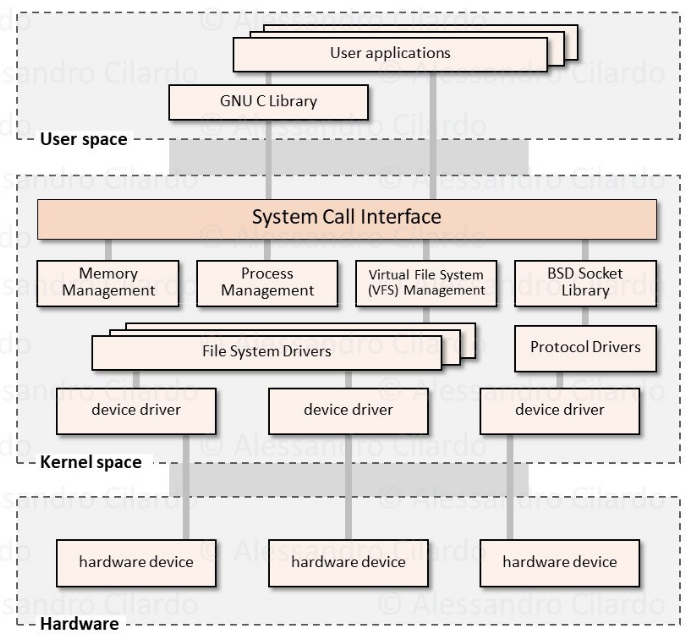
\includegraphics[width=.65\textwidth]{figures/ch2/linux-architecture.png}
  \end{center}
  \caption{Architettura del kernel Linux}\label{fig:linux-architecture}
\end{figure}

\paragraph{Gestione della memoria}
Linux gestisce uno spazio di indirizzamento a $32-bit$ ($4GB$) e prevede che la parte bassa partendo dal basso ($0x00000000-0xBFFFFFFF$, $3GB$) sono dedicati allo \textit{user space}, mentre quelli alti ($0xC0000000-0xFFFFFFFF$, $1GB$) al \textit{kernel space} che include una sezione per l'I/O ed è quella che viene utilizzata quando c'è una system call da un processo utente che, pur restando nel processo utente, obbliga il processore a passare dalla modalità utente alla modalità supervisore. Nella parte \textit{user space}, gli indirizzi vengono tradotti con una MMU, ma in quelli \textit{kernel space} la traduzione viene bypassata e le system call vengono intercettate con delle eccezioni gestite con un opportuno handler che va a controllare un struttura dati detta \textbf{\textit{system call table}}. Questo meccanismo viene fornito attraverso un'interfaccia detta \textbf{\textit{System Call Interface}} (\cref{fig:linux-architecture}).

\paragraph{File System}
Linux si caratterizza dal fatto di avere un supporto molto ricco e molto vario per il \textbf{\textit{file system}} inteso come regole per la gestione dello storage grezzo che si può avere sul dispositivo, ed è utile in tanti contesti tra cui la Zynq in cui ce ne sono di diversi come una SD, una flash. In realtà, quello che rende anche molto flessibile l’architettura di Linux è il ricondurre alla gestione del file system anche meccanismi di interazione che non sono propriamente la gestione dello storage. Innanzitutto, Linux prevede una struttura basata sul concetto di \textbf{\textit{virtual file system}} che fornisce un’astrazione superiore rispetto a quella del semplice file systeml, quindi la gerarchia di file system che possono essere montati (o anche smontati all’occorrenza) possono essere eterogenei. Per esempio, \textbf{\textit{procfs}} e \textbf{\textit{sysfs}} sono tipicamente montati sotto \textbf{\textit{/proc}} e \textbf{\textit{/sys}} rispettivamente, in realtà non sono materialmente dei file  ma sono un’astrazione nella forma di file system di una serie di informazioni che il kernel rende disponibili ed espone agli utenti. Nel caso \textit{sysfs}, le informazioni di configurazione del sistema che potrebbero essere la configurazione della cache, della \textit{SMMU}, del meccanismo di traduzione degli indirizzi, e fondamentalmente in forma di file che hanno specifici nomi e specifici percorsi, possiamo leggere (e in qualche caso anche scrivere) informazioni che sono relative alla gestione del sistema fatta dal kernel in collaborazione col processore. L'interazione con i dispositivi è incanalata in un’astrazione che è quella del file system: interagire con un dispositivo significa, interagire con un file system ovvero con un API standard in cui ci sono le primitive \textit{read, open, close, write ecc}.

\paragraph{Driver}
In Linux, c'è supporto per molti tipi di dispositivi con \textit{driver built-in}. Quando i dispositivi erano limitiati questi venivano caricati in memoria al boot, ma ora c'è un meccanismo di caricamento dinamico; tuttavia è possibile avere dei \textit{driver} \textbf{\textit{compiled-in}}. In Linux, i driver sono caricati nel kernel sottoforma di \textbf{\textit{kernel object (.ko)}}. Questo consente al kernel di essere leggero e veloce da avviare ed è possibile sviluppare con più facilità. Inoltre, c'è una distinazione tra $3$ tipi di dispositivi che espongono API diverse:
\begin{itemize}
  \item dispositivi a caratteri: questo tipo di dispositivi realizzano uno \textit{stream} di \textit{byte};
  \item dispositivi a blocchi: hanno la nozione di trasferimento di blocchi di dati di varie dimensioni e potrebbero interagire con un DMA;
  \item dispositivi di rete: rendono espliciti la nozione di \textit{socket}
\end{itemize}

\paragraph{Sequenza di boot}
Quando si preme il pulsante di accensione, si effettua il cosiddetto \textbf{\textit{stage 0 boot}}. Da una ROM o una Flash on chip si carica l'indirizzo con cui far partire il \textbf{\textit{BIOS} (Basic Input Ouput System)} nel quale vengono fatte attività di \textit{self test}.
Fondamentalmente si passa la palla a un layer successivo che prende il nome di \textbf{\textit{First Stage Boot Loader (FSBL)}} che sulla Zynq può essere cifrato e autenticato con HMAC. Su sistemi tradizionali, il boot dopo la prima routine eseguita dal firmware sulla nostra memoria non volatile, viene poi fatto a partire da un disco, sul quale ci si aspetta di trovare un settore (il primo, da $512b$, chiamato \textbf{\textit{Master Boot Record (MBR) }}) che contiene nei limiti della sua dimensione il FSBL tradizionale (diversi byte con anche un checksum e come andare a recuperare lo stage successivo). In realtà, da diversi anni non è più quello che accade, perché oltre a questo approccio legacy esiste un approccio più sofisticato (\textbf{\textit{UEFI}}) che supera questi limiti prevede di standardizzare la catena di boot comprendendo anche aspetti di sicurezza che ovviamente sono fondamentali perché questo è il momento iniziale dal quale poi possono partire diverse strade, e un attacco fatto a questo livello potrebbe essere anche abbastanza critico.

\begin{figure}
\centering
\begin{subfigure}{.5\textwidth}
  \centering
  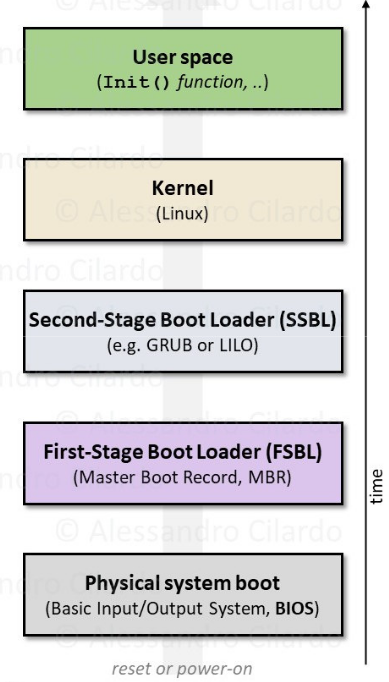
\includegraphics[width=.5\linewidth]{figures/ch2/generic-boot.png}
  \caption{Boot generico}
  \label{fig:generic-boot}
\end{subfigure}%
\begin{subfigure}{.5\textwidth}
  \centering
  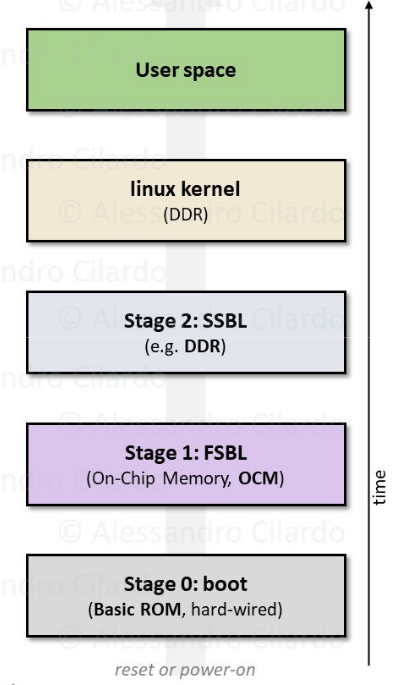
\includegraphics[width=.5\linewidth]{figures/ch2/zynq-boot.png}
  \caption{Boot della zynq}
  \label{fig:zynq-boot}
\end{subfigure}
\caption{Sequenza generica di boot e particolarizzato con la zynq}
\end{figure}

Il \textbf{\textit{Second Stage Boot Loader (SSBL)}} è fondamentalmente la schermata con le diverse opzioni di boot con diversi kernel. Tra le altre cose il SSBL si incaricherà anche di individuare quale kernel caricare, quindi potrebbe anche chiederlo a noi. In \cref{fig:generic-boot}, c'è LILO che è il più vecchio di linux che agisce come SSBL, mentre quello più recente è GRUB, più sofisticato, che permette di cercare l’immagine del kernel in determinati file system conoscendoli e sapendoli interpretare. E’ un’evoluzione utile quella tra LILO e GRUB perché a GRUB posso dare in pasto uno storage formattato, cosa che altrimenti non poteva accadere. Quindi quantomeno il SSBL può avere un’interfaccia, la possibilità di individuare quale kernel utilizzare, può anche fare cose più sofisticate dal punto di vista del controllo, ad esempio dell’integrità del kernel. Chiaramente sul SSBL non ci sono problemi di dimensione e può essere anche più ricca e sofisticata l’interfaccia esposta dall’SSBL o la logica che applica. In ogni caso quello che deve fare è individuare il kernel (proprio come file all’interno di un file system) e poi si passa alla fase successiva in cui il kernel comincia a fare i suoi settaggi di aspetti quali cache, traduzione degli indirizzi, rilevamento delle caratteristiche del processore, ad esempio supporto della floating point unit o meno, e infine il kernel linux invoca una funzione che si chiama \textbf{\textit{init}} che è la prima ad essere eseguita in user space (tra l’altro, è anche la prima che viene scritta internamente appoggiandosi su una libreria c, mentre tutto il resto è scritto con la filosofia legacy di compilare senza nemmeno una include, e senza poter usare nessuna delle funzioni della libreria standard del c). La \textbf{\textit{init}} è la prima che si basa sulla libreria c e quindi deve essere stata chiaramente opportunamente caricata e tra le altre cose che fa, in uno speciale percorso individuato dal kernel, in un file all’interno di questo percorso ci troviamo una entry che determina anche quello che si chiama il \textit{runlevel}, quindi una di diverse possibili modalità nelle quali carico un kernel:
\begin{itemize}
  \item single-user;
  \item mult-user;
  \item no-network;
  \item debug;
\end{itemize}

Questo processo può essere personalizzato per diverse board come la Zynq (\cref{fig:zynq-boot}). Nel SoC non c'è il BIOS, ma un qualcosa di equivalente che viene cablato all'interno in una flash interna non modificabile detta \textbf{\textit{boot ROM}}. Questa viene bruciata da Xilinx e contiene poche istruzioni necessarie a passare al FSBL che si trova in una memoria interna. L'FSBL può essere manomesso e Xilinx offre dei meccanismi per verificarne l'integrità con HMAC o cablando un hash all'interno del SoC o usando la crittografia a chiave asimmetrica e firmare digitalmente l'FSBL. Per essere eseguito FSBL deve essere in RAM detta \textbf{\textit{On Chip Memory} (OCM)} e non può essere più grande (tipicamente $192kb$). È prevista una modalità detta \textbf{\textit{FSBL-in-place}} come nel Cortex-M in cui FSBL viene eseguito direttamente dalla flash e dovrebbe essere utilizzato solo in fase di debug. La \textit{boot rom} legge un bit in cui si dice come eseguire l'FSBL.

Caricato l'FSBL in OCM, bisogna creare la piattaforma. In questa fase, se esiste viene caricato il \textbf{\textit{bitstream}} dell'FPGA (che può essere cifrato e/o firmato digitalmente tramite un HMAC. FPGA ha hardware che effettua AES e HMAC). Il SoC deve mettere a disposizione meccanismi per gestire in sicurezza le chiavi come BBRAM e eFUSE (discusse in \cref{sec:security}). Verificata la parte di sicurezza, si passa al \textit{SSBL} per caricare Linux (nei sistemi embedded non si usa ne LILO ne GRUB, ma \textbf{\textit{u-BOOT}}).

Come mostrato in \cref{fig:generic-boot-format}, il file principale è \textit{boot.ini}. Questo deve contenere FSBL (.elf), il bitstream (.bit) e il SSBL (.elf). Se si vuole eseguire un'applicazione bare metal, allora SSBL può caricare la prima istruzione del programma. Altrimenti, bisogna caricare un'immagine del kernel (\textit{zImgage}, da caricare in RAM) che deve inclusa nel \textbf{\textit{boot medium}}. Oltre all'immagine è necessario avere un \textbf{\textit{ramdisk}} utilizzato per dedicare una porzione di RAM a come se fosse un disco (per creare un virtual filesystem). Infine, la parte più interessante è svolta dal \textit{device-tree.dtb} (\textit{device tree blob}). Questo file è la descrizione della configurazione hardware sottostante inclusiva dei processori, delle parti più stabili, ma anche delle periferiche, in particolare quelle che ho aggiunto io. Questo elemento permette di disaccoppiare kernel (la \textit{zImage}, scritto senza preoccuparsi delle molteplici possibilità che una board o dispositivo in generale può offrire) e un layer che viene letto dal kernel a tempo di boot per apprendere fisicamente come è configurata la piattaforma sottostante.

\begin{figure}
\centering 
\begin{subfigure}{.5\textwidth}
  \centering
  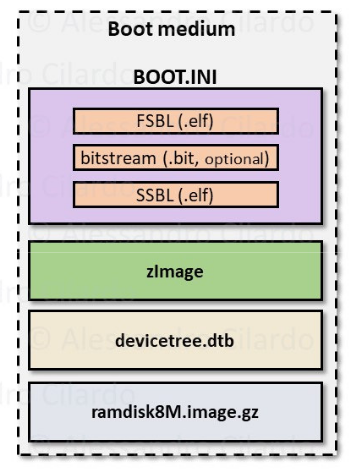
\includegraphics[width=.5\linewidth]{figures/ch2/zynq-boot-basic.png}
  \caption{Struttura del boot medium}
  \label{fig:generic-boot-format}
\end{subfigure}%
\begin{subfigure}{.5\textwidth}
  \centering
  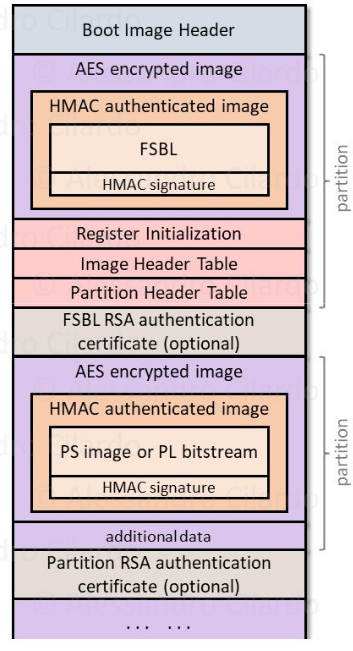
\includegraphics[width=.5\linewidth]{figures/ch2/zynq-boot-format.png}
  \caption{Dettaglio del boot medium}
  \label{fig:zynq-boot-format-detail}
\end{subfigure}
\caption{Struttura del file di configurazione di boot per la Zynq}
\end{figure}

Questo file contiene in maniera gerarchica, sotto forma di albero, la struttura fisica del sistema processori, bus intesi come raggruppamenti di periferiche omogenee (non necessariamente un bus fisico ma un’astrazione che viene esposta al kernel quando legge questo file) e ci sono informazioni riguardanti le periferiche come registri di occupa, cioè quali indirizzi fisici corrispondono ai registri di quella periferica. Ovviamente non si indicano tutti i registri, ma quelli fondamentali come indirizzo base, dimensione della finestra, numero di interruzione associato. Il device tree descrive sia la parte PS che quella PL. In \cref{fig:device-tree-basic}, c’è una regione che riguarda la cpu, che mostra le scelte specifiche che sulla mia board faccio per configurare alcuni parametri della cpu (parte PS quindi), poi c’è la parte di periferiche indicata con ps7. All'inizio si definiscono i controller delle interruzioni, le CPU e poi le periferiche. Ad ogni elemento è associato un oggetto con le proprietà dette in precedenza. Da notare la stringa \textit{compatible} che serve a fare match con il driver.  Il kernel si crea una tabella cin queste informazioni per capire quale driver assegnare a ciascuna periferica. 

\begin{figure}
  \begin{center}
    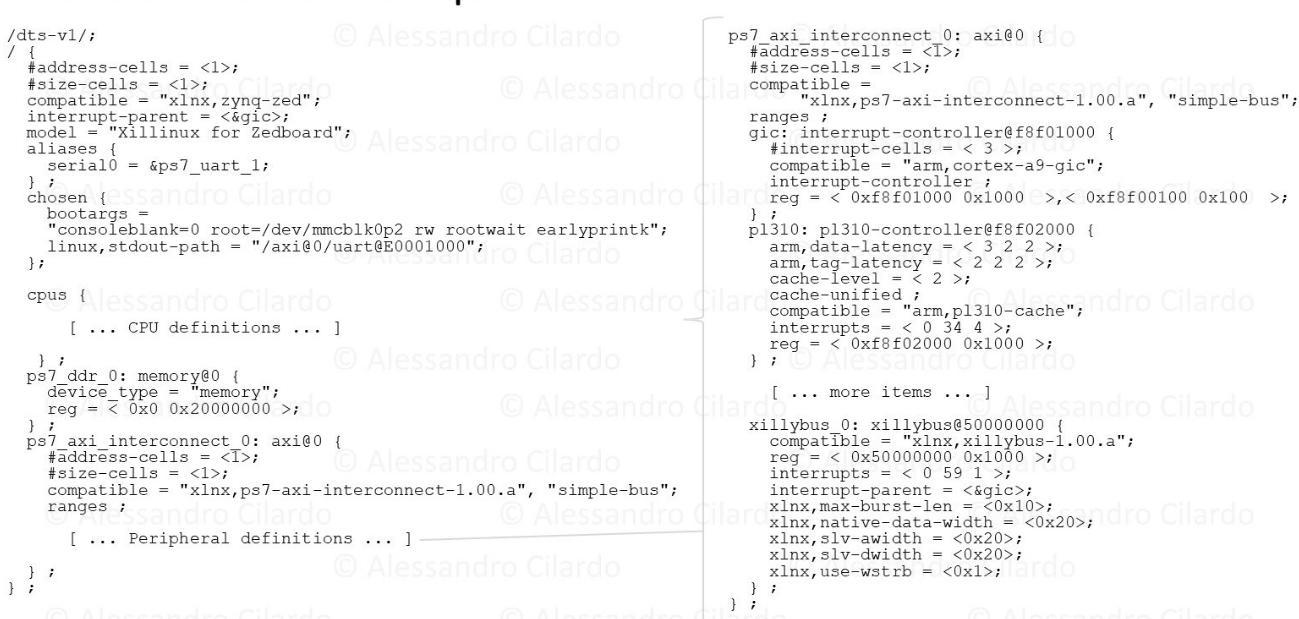
\includegraphics[width=0.95\textwidth]{figures/ch2/device-tree-basic.png}
  \end{center}
  \caption{Esempio di device tree}\label{fig:device-tree-basic}
\end{figure}

Il DTB viene compilato da un \textbf{\textit{Device Tree Compiler (DTC)}} che in ingresso più file detti \textbf{\textit{Device Tree Source} (DTS)} . Questo lo si fa spesso perché alcuni file possono esseere comuni a più board e possono definire dei dispositivi segnaposto che possono essere sovrascritti da altri file o disabilitandoli se non supportati.

\clearpage
\section{Aspetti avanzati}
\subsection{Virtualizzazione}\label{sec:virtualization}
Il focus è sulla virtualizzazione in ARM. Di seguito, vengono prima dati dei riferimenti storici per capire il problema della virtualizzazione e cosa è stato provato da Intel e AMD per l'architettura $x86$.
\subsubsection{Introduzione}
La virtualizzazione è una tecnica utilizzata per condividere la stessa piattaforma tra sistemi operativi diversi. Un sistema virtualizzato si dice che ospita delle macchine virtuali. Le macchine virtuali sono gestite da un \textbf{Virtual Machine Monitor (VMM)} detto anche \textbf{hypervisor}.
In generale, ciò porta diversi benefit quali:
\begin{itemize}
  \item \textbf{safety e security}: guasti, bug e azioni malevoli su una macchina virtuale non impattano le altre. Questa proprietà è detta \textbf{sandboxing};
  \item coesistenza di diversi sistemi operativi sulla stessa piattaforma. Ciò può essere utile anche per supportare sistemi legacy
  \item motivi economici: costa molto meno alimentare macchine diverse. Una macchina occupa meno spazio e può essere gestita facilmente
  \item load balacing: è più facile gestire (replicare) stack applicativi per la migrazione di processi ecc; 
  \item developer experience: è molto più facile testare un'applicazione sotto diversi sistemi operativi;
\end{itemize}

Ci sono $2$ tipi di Hypervisor (\cref{fig:type-of-hypervisors}):
\begin{enumerate}
  \item Hypervisor di tipo $1$: funziona solo a contatto con hardware. È detto anche hypervisor \textbf{bare metal};
  \item Hypervisor di tipo $2$: funziona insieme ad un sistema operativo \textbf{host}. Si parla di hypervisor \textbf{hosted};
\end{enumerate}
Il problema principale di un sistema virtualizzato sta nel fatto che le macchine virtuali credono di essere l'elemento più privilegiato all'interno del sistema. Infatti, un sistema operativo è formato da una parte \textbf{kernel mode} (privilegiata) e una \textbf{user mode}. Un sistema in \textit{kernel mode} ha il controllo totale sulla parte hardware. Chiaramente non è possibile avere più sistemi kernel mode contemporaneamente ed è qui che il VMM interviene per rendere possibile la coesistenza di diversi kernel.

\begin{figure}[h]
  \begin{center}
    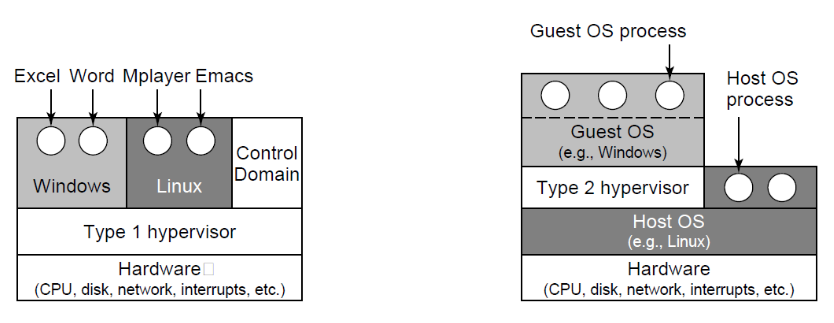
\includegraphics[width=.7\textwidth]{figures/ch3/virtualization/hypervisors.png}
  \end{center}
  \caption{Tipi di hypervisors}\label{fig:type-of-hypervisors}
\end{figure}

\paragraph{Requisiti formali per la virtualizzazione}
Dal punto di vista formale, \href{https://en.wikipedia.org/wiki/Popek_and_Goldberg_virtualization_requirements}{Popek e Goldeberg} enunciarono i requisiti principali per supportare la virtualizzazione. Innanzitutto, viene fatta una distinzioni tra le istruzioni di una CPU: non tutte sono uguali e su alcune di queste deve agire l'hypervisor.
In particolare, le \textbf{sensitive instructions} indicano istruzioni per accedere all'I/O, impostazioni dell'MMU e tutte le altre che devono essere eseguite in  \textit{kernel mode} e non è possibile eseguire in \textit{user mode}. Le \textit{privileged instructions} sono quelle istruzioni che se eseguite in modalità utente (e devono essere in modalità kernel) generano una trap. Nell'articolo, è mostrato che una macchina è virtualizzabile solo se le \textit{sensitive instructions} sono un sottoinsieme di quelle \textit{privileged}. Questo concetto abilita la tecnica del \textbf{\textit{trap and emulate}} per eseguire un sistema virtualizzato.

Questo articolo dimostra anche che la prima architettura x86 non è fatta per essere virtualizzata. Infatti, molte \textit{sensitive instructions} non eseguivano trap. Ad esempio, l'accesso a registro di stato da parte di un processo utente si traduceva semplicemente in una \textit{no-op}. Il supporto hardware alla virtualizzazione detta \textbf{VT} per Intel e \textbf{SVM} per AMD fu introdotto a partire dal $2005$.

\paragraph{Virtualizzazione senza supporto hardware: binary translation}
Senza supporto hardware, vengono usati sia la \textbf{binary translation} che i \textbf{protection ring}. L'architettura x86 ha $4$ protection mode. In un sistema non virtualizzato, il ring $0$ viene dato al kernel e i processi utente vengono eseguiti in in ring $3$. Parlando di hypervisor bare metal, le macchine virtuali usavano il ring $1$, mentre quello $0$ viene assegnato all'hypervisor (modello $0/1/3$, \cref{fig:x86-ring-deprivileging}).

\begin{figure}[h]
  \begin{center}
    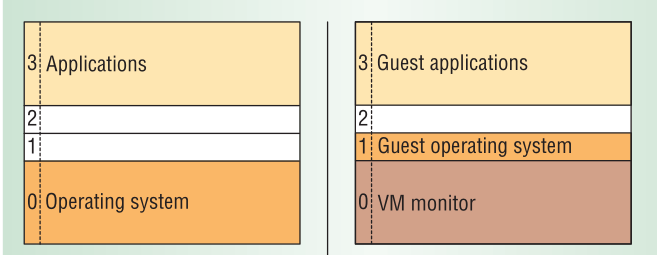
\includegraphics[width=.75\textwidth]{figures/ch3/virtualization/x86-ring-deprivileging.png}
  \end{center}
  \caption{Tecnica del ring-deprivileging prima di Intel-VTx}\label{fig:x86-ring-deprivileging}
\end{figure}

La binary translation consiste nel tradurre \textbf{basic blocks} (pezzi di codice senza salti, chiamate a funzione, trap ecc) in istruzioni compatibili. Prima dell'esecuzione di un pezzo di codice, l'hypervisor esamina il codice e, se questo contiene istruzioni sensitive, le rimpiazza con chiamate alle procedure dell'hypervisor che le gestiscono. 
Questa operazione può sembrare onerosa, ma le traduzioni sono memorizzate e le \textbf{sensitive instruction} sono una minima parte del codice da virtualizzare. Infatti, essa non interviene con i processi utente, ma solo con quelli che eseguono in \textit{kernel mode}.

Questa tecnica è semplice e si presta bene alle ottimizzazioni. Ad esempio, se un blocco tradotto termina, o viene concatenato con un'altra istruzione sensitiva, si può evitare di dare il controllo all'hypervisor. Inoltre, in alcune implementazioni si preferisce usare questa approccio anche per le parti che dovrebbero eseguire in \textit{trap and emulate} perché le trap invalidano le \textit{cache} e, hanno performance peggiori della traduzione dei blocchi. In generale, queste considerazioni hanno senso anche in hypervisor di tipo $2$. Il controllo hardware viene effettuato attraverso moduli kernel che comunicano con il sistema operativo host.

Un modello simile a quello mostrato è quello in cui viene utilizzato il livello di privilegio $3$ sia per i kernel delle macchine virtuali sia per i guest; mentre il VMM esegue a ring $0$ (modello $0/3/3$).

La virtualizzazione con  \textit{ring deprivileging} ha molti problemi che non possono essere risolti via software senza impattare di molto le performance dei guest o violando i principi di \textit{fidelity} di un VMM. Alcune di questi problemi riguardano:
\begin{itemize}
  \item \textbf{\textit{Ring aliasing}}: quando un'istruzione viene eseguita ad un ring diverso da quella per cui è stata pensata. Un guest OS può semplicemente ispezionare dei registri per capire che non sta eseguendo con privilegio $0$
  \item \textbf{\textit{Address-space compression}}: i sistemi operativi si aspettano di poter operare su tutto lo spazio di indirizzamento virtuale, ma ciò non è possibile. Il VMM ha bisogno di un suo spazio di indirizzamento e deve anche prendere un po' di memoria dai guest perché ha bisogno di allocare codice e strutture dati per gestire i cambi di contesto. Quindi bisogna prevenire che i guest entrino in queste aree di memoria protette
  \item \textbf{\textit{Non faulting access to privileged state}}: alcune istruzioni possono eseguire anche in modalità utente e possono accedere a strutture dati critiche a ring $0$. L'accesso a queste strutture come il registro $PTA$ (che contiene l'indirizzo della \textbf{Virtual Hash Page Table (VHPT)}) può far capire al guest di non essere da solo nel sistema e non avere il pieno controllo della CPU
  \item \textbf{\textit{Adverse impacts on guest transitions}}: non è possibile utilizzare le istruzioni \textit{SYSENTER} e \textit{SYSEXIT} per avere system call a bassa latenza. Queste istruzioni portano sempre ad eseguire in ring $0$ che non corrisponde alla modalità corretta per i guest. Un guest che usa \textit{SYSENTER} non va in \textit{kernel mode}, ma nel VMM. Il VMM deve poter emulare queste due istruzioni. Inoltre, l'architettura Intel supporta interruzioni veloci che non mettono dati in memoria, ma passano informazioni sull'interruzione in registri del processore. Tutti gli interrupt handler usano questi registri. Nel caso virtualizzato si genererebbero molte trap che devono essere intercettate e gestite dal VMM
  \item \textbf{\textit{Ring compression}}: per proteggere il VMM bisogna usare un meccanismo di protezione della memoria: paging. Per come è fatta, la tabella delle pagine in IA-32 non distingue i livelli di privilegio tra $0-2$. Questo vuol dire che il guest OS deve eseguire a livello $3$ per non impattare il VMM
  \item \textbf{\textit{Access to hidden state}}: alcuni registri del processore non possono essere acceduti via software. Quindi ci potrebbero essere problemi di sicurezza tra guest. Il VMM non è in grado di ripristinare questi registri
\end{itemize}

\paragraph{Supporto hardware alla virtualizzazione: Intel VT-x}
Tutti i problemi visti nel caso precedente vengono presi in considerazione in Intel VT-x. Questa estensione dell'architettura si basa sull'introduzione due modalità operative: \textbf{VMX root} e \textbf{VMX non root}. Un VMM esegue in \textit{VMX root}, i guest in \textit{VMX non root}. In queste due modalità operative, entrambi hanno i $4$ livelli di privilegio. Vengono definiti due passaggi di stato $\text{VMX root} \to \text{VMX non root}$ \textbf{\textit{VM entry}} ; mentre $\text{VMX non root} \to \text{VMX root}$ \textbf{\textit{VM exit}}.

Il sistema in modalità \textit{VMX root} è simile al sistema senza VTx. In modalità, VMX non root molte istruzioni generano dei VM exit (alcuni senza condizione altri con l'aiuto di altri registri). VTx mette a disposizione una nuova struttura di controllo \textit{Virtual Machine Control Structure (VMCS)} divisa in due parti: una per i guest e una per l'host.

Un'altra aggiunta sono \textit{VM-execution control fields} che consentono di configurare il processore in modo da specificare quali sono le istruzioni che causano VM exit e protezioni aggiuntive per i registri $CR3$, $CR4$ ecc. Altri controlli abilitano le interrupt virtuali. Tutte le interrupt esterne causano VM exits. Altri controlli sono costituiti da bitmap che consentono di gestire quando deve essere eseguito un VM exits in base a istruzioni I/O o eccezioni.

\paragraph{Virtualizzazione della memoria senza supporto hardware: shadow page tables}
Per esempio se un guest decide di mappare le pagine $7,4,3$ sulle pagine fisiche $10,11,12$, e, analogamente un altro guest decide di mappare le sue pagine $4,5,6$ su $10,11,12$. Cosa deve fare un VMM per gestire l'allocazione fisica delle pagine? Non può allocare la stessa pagina fisica. Si dice che il VMM crea una \textbf{\textit{shadow page table}} per ogni guest. Il problema principale di questo approccio sta nel fatto che il guest può cambiare la sua tabella delle pagine semplicemente scrivendo in memoria e non c'è modo per il VMM di saperlo.

Tutti i modi in cui il VMM può usare per tenere traccia delle pagine di memoria dei guest sono costosi poiché richiederebbero tanti page fault. Sono due strategie principali:
\begin{itemize}
  \item aspettare che il guest acceda alle pagine. Aggiornare la shadow page table e far riprendere l'esecuzione. Non funziona con la cancellazione: se una pagina viene cancellata questa non sarà mai più acceduta dal guest;
  \item creare una top level table page e usare le sensitive instruction del guest che accede al registro della top level table page per aggiornare la shadow page table.
\end{itemize}
Visto che queste due tecniche generano tanti page fault, bisogna distinguere i veri page fault (il guest che prova a prendere una pagina dal disco perchè non presente in RAM, noti come \textit{guest-induced faults} e quelli del VMM che tiene aggiornata la shadow page table (\textit{hypervisor-induced page faults}).

\paragraph{Virtualizzazione della memoria con supporto hardware: extended page tables}
EPTs (Extended Page Tables) (\cref{fig:x86-epts}) ha come obiettivo quello di rimuovere le trap per accedere alla memoria. Bisogna distinguere tra \textbf{\textit{guest physical addresses}}, \textbf{\textit{guest virtual address}} e \textbf{\textit{host physical address}}. Molto del lavoro per gestire le shadow page table adesso viene fatto dalla CPU in hardware analogamente a come viene fatto senza VM. L'unica differenza sta nel fatto che adesso la tabella delle pagine è più complicata e viene messa una grossa pressione sul TLB.

\begin{figure}[ht]
  \begin{center}
    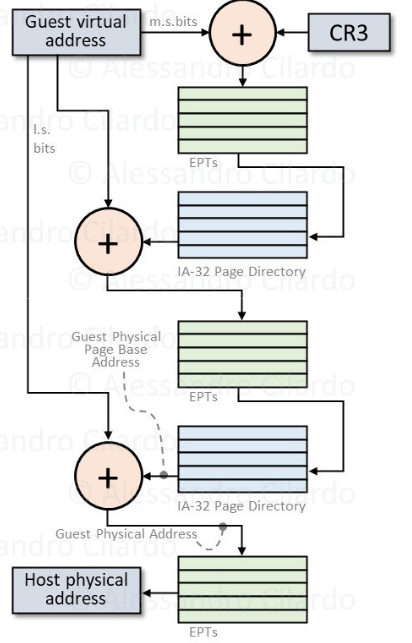
\includegraphics[width=.4\textwidth]{figures/ch3/virtualization/x86-epts.png}
  \end{center}
  \caption{Meccanismo delle Extended Page Tables}\label{fig:x86-epts}
\end{figure}


\subsubsection{Virtualizzazione in ARMv8-A}
ARMv8-A introduce il concetto di \textbf{\textit{Address Space}}(\cref{fig:armv8-a-address-spaces}) ciascuno contraddistinto da un'etichetta che precede l'indirizzo virtuale a cui si sta tentando di accedere. L'etichetta è fatta da due parti:
\begin{itemize}
  \item \textbf{Secure} o \textbf{Non Secure}: NS indica non secure;
  \item \textbf{\textit{Exception Level}} EL;
\end{itemize}

Ad esempio, un indirizzo virtuale potrebbe essere \textit{NS.EL2:0x8000}. In particolare ARMv8-A, presenta $3$ address spaces:
\begin{itemize}
  \item NS.EL0-NS.EL1 (esiste anche la versione sicura EL0-EL1);
  \item NS.EL2 (con il corrispondente valore sicuro EL2);
  \item EL3;
\end{itemize}

Ogni \textit{address space} ha le proprie tabelle (che funzionano come un normale TLB) e configurazioni che sono puntate dal registro \textit{Translation Table Base Register} (\textbf{TTBR}). I TTBR sono disponibili anche in versione virtuale e in tal caso sono gestiti dall'hypervisor. 

Guardando la \cref{fig:armv8-a-address-spaces}, si nota che per NS.EL0 e NS.EL1 è previsto un ulteriore stage di traduzione. Infatti, dal primo stage si nota che questi condividono la stessa tabella la cui uscita è un \textbf{\textit{Intermediate Physical Address (IPA)}} che a sua volta viene tradotto da un'altra tabella memorizzata in un \textbf{vTTBR0\_EL2} (interviene l'hypervisor). La presenza degli IPA crea un'ambiguità nei TLB che può essere risolta o con gli \textbf{Address Spacer Identifier} (ASID) che da un \textbf{Virtual Machine Identifier} (VMID). In generale, non è detto che questi nomi siano consistenti tra diversi core. Inoltre, questo è molto importante in single-core poichè in ARMv8-A è presente una forma di \textit{hyper-threading} in cui duplicando parte del \textit{register file} è possibile avere un'implementazione hardware di un thread eseguendo di fatto due istruzioni per volta. Questi componenti vengono detti \textbf{virtual cpu} (o \textit{virtual processing element}), ma non c'entrano nulla con la virtualizzazione, e condividono lo stesso TLB quindi c'è bisogno di risolvere l'ambiguità.

\begin{figure}[H]
  \begin{center}
    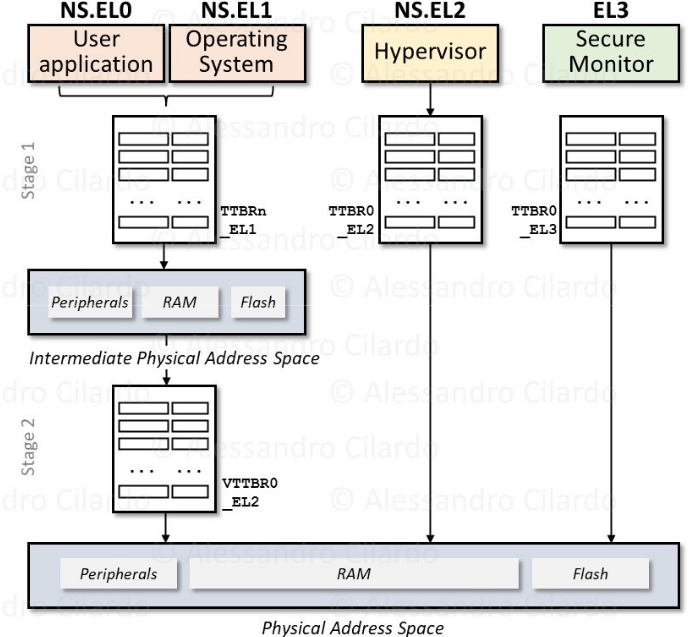
\includegraphics[width=.6\textwidth]{figures/ch3/virtualization/armv8-address-spaces.png}
  \end{center}
  \caption{Address spaces in ARMv8}\label{fig:armv8-a-address-spaces}
\end{figure}

Gli indirizzi utilizzati sono sempre a $64-bit$, ma la memoria disponibile è effettivamente inferiore. L'organizzazione degli indirizzi non cambia tanto per i livelli bassi: lo spazio viene partizionato in user space e kernel space (si utilizzano tutti e $64-bit$), mentre per i livelli più alti non c'è questa distinzione (in base all'implementazione si può arrivare fino a $52-bit$). Se il bit di configurazione $E2H = 1$ allora è possibile avere user/kernel space anche in EL2 e ciò risulta particolarmente utile quando si vuole installare un hypervisor \textit{hosted} mantenendo il sistema operativo host in EL2.

Come detto in precedenza il TLB è una cache delle traduzioni: ciò significa che un sistema operativo che effettua un cambio di contesto o cambia una pagina nella effettiva tabella deve invalidare le \textit{entry}. A tal proposito ARMv8, mette a disposizione un'istruzione speciale $TLBI$ che consente di invalidare selettivamente delle entry del TLB. Questa è un'operazione molto costosa poichè deve essere preceduta da istruzioni di barriera per essere sicuri che la \textit{pipeline} sia vuota. In \cref{fig:tlb-invalidation}, è mostrato un esempio di scrittura nella tabella e l'invalidamento del TLB.

\begin{figure}[h]
  \begin{center}
    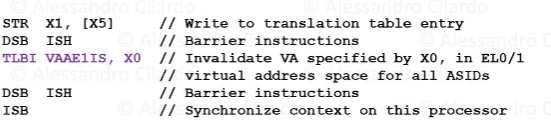
\includegraphics[width=.5\textwidth]{figures/ch3/virtualization/armv8-tlb-invalidation.png}
  \end{center}
  \caption{Programma che modifica la tabella di traduzione ed invalida il TLB dopo un'istruzione di tipo \textit{memory barrier}}\label{fig:tlb-invalidation}
\end{figure}
\clearpage

\paragraph{Virtualizzazione I/O in ARMv8}
La traduzione a due livelli rende più complicato la virtualizzazione dell'I/O. Ad esempio, se una macchina virtuale accede ad una periferica, l'attributo di memoria del \textit{Virtual Address Space} è quello di \textbf{device} (\cref{fig:armv8-memory-attributes}); mentre la periferica emulata sarà vista come un'area di memoria nell'host fisico e quindi avrà come attributo \textbf{normal}. Ci sono delle regole stringenti che ARM impone per fare questa traduzione.

\begin{figure}[ht]
  \begin{center}
    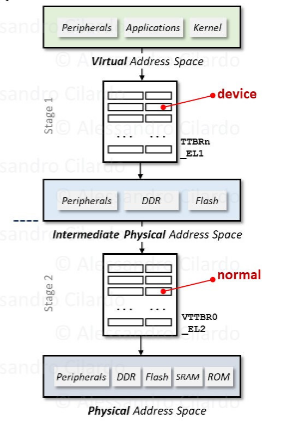
\includegraphics[width=.4\textwidth]{figures/ch3/virtualization/armv8-memory-attributes.png}
  \end{center}
  \caption{Attributi di memoria in una traduzione a $2$ livelli in ARMv8}\label{fig:armv8-memory-attributes}
\end{figure}

Inoltre, è possibile collegare una periferica fisica ad una macchina virtuale (magari assegnata in esclusiva). In questo caso, si vuole collegare l'IPA direttamente alla periferica nello spazio fisico. Per fare ciò bisogna assegnare alla periferica l'indirizzo fisico in \textbf{stage 2} (\cref{fig:armv8-peripheral-emulation}). 

\begin{figure}[H]
  \begin{center}
    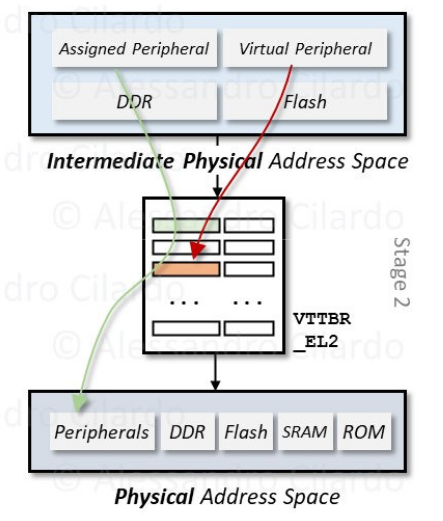
\includegraphics[width=.35\textwidth]{figures/ch3/virtualization/armv8-peripheral-emulation.png}
  \end{center}
  \caption{Traduzione di livello $2$ per una macchina virtuale con una periferica assegnata}\label{fig:armv8-peripheral-emulation}
\end{figure}

Quando la macchina virtuale che accede a questo indirizzo fisico in \textbf{stage 1} genererà un'eccezione (\textit{page fault}) che verrà gestita dall'hypervisor tramite un \textbf{ABORT} in EL2 e viene popolato il registro \textbf{ESR\_EL2} con tutte le informazioni utili (indirizzo acceduto, operazione effettua ecc), mentre in \textbf{HPFAR\_EL2} viene inserito l'IPA che ha generato l'accesso. L'hypervisor usa questi due registri per risalire alla periferica virtuale e l'operazione viene emulata (\cref{fig:armv8-peripheral-emulation-detail}).

\begin{figure}[h]
  \begin{center}
    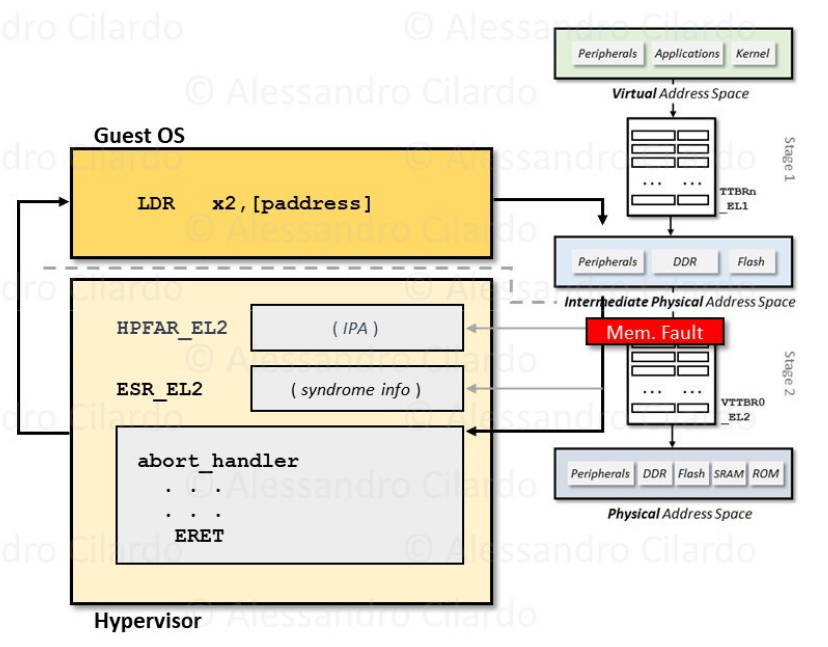
\includegraphics[width=.55\textwidth]{figures/ch3/virtualization/armv8-peripheral-emulation-detail.png}
  \end{center}
  \caption{Accesso ad una periferica fisica e gestione da parte dell'hypervisor}\label{fig:armv8-peripheral-emulation-detail}
\end{figure}

Il discorso si complica quando non c'è solo il core che vuole accedere al dispositivo fisico, ma altri dispositivi come DMA. Di fatto, il DMA fa le veci del core e quindi deve accedere anche lui ai registri fisici. In questo caso, ARM prevede l'introduzione di un'altra unità detta SMMU (o \textbf{\textit{IOMMU}}) che deve essere configurato dall'hypervisor per far vedere le IPA del guest come pagine dell'host al DMA (\cref{fig:armv8-dma-iommu}.

\begin{figure}[h]
  \begin{center}
    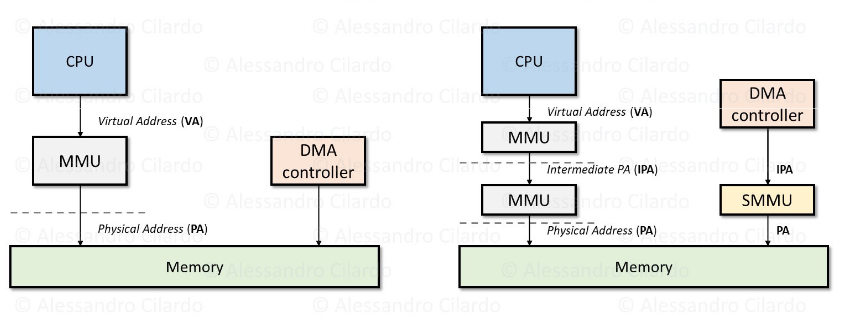
\includegraphics[width=.9\textwidth]{figures/ch3/virtualization/armv8-dma-iommu.png}
  \end{center}
  \caption{Introduzione IOMMU per consentire ad altri master di accedere alle IPA dei guest}\label{fig:armv8-dma-iommu}
\end{figure}

\paragraph{Virtualizzazione di un eccezione}
Alcuni tipi di eccezioni devono essere gestite dall'hypervisor, ma altre da una specifica VM (che potrebbe non essere in esecuzione quando si verifica l'eccezione). Nell'ultimo caso, bisogna inoltrare l'eccezione alla macchina virtuale (o ad una specifica vCPU assegnata alla VM). In questo senso, ARMv8 supporta le \textit{virtual interrupts} (\textit{vIRQ, vFIQ e vSErrors}). In generale, esistono due modi per generare un'interruzione virtuale:
\begin{itemize}
  \item si configurano dei bit in $HCR\_EL2$ per sollevare vIRQ, vFIQ e vSError (ovvero si alza un bit in vCPU). È semplice, ma il controller delle interruzioni nel \textit{guest}viene comunque emulato attraverso l'hypervisor e quindi sarebbe inefficiente;
  \item si utilizza il GIC. L'hypervisor registra una vCPU come se fosse una CPU semplice. In questo modo, la VM comunica direttamente con il GIC \cref{fig:virtual-exception-generation-gic}
\end{itemize}

\begin{figure}[h]
  \begin{center}
    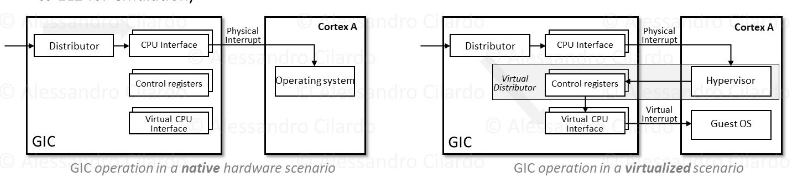
\includegraphics[width=.85\textwidth]{figures/ch3/virtualization/virtual-exception-generation-gic.png}
  \end{center}
  \caption{Registrazione di una vCPU nel GIC}\label{fig:virtual-exception-generation-gic}
\end{figure}


\paragraph{Cenni di virtualizzazione sicura} 
In ARMv8.4, la virtualizzazione sicura si basa sulla possibilità di installare \textit{trusted firmware} in EL3. Nelle versioni precedenti, EL3 conteneva firmware e codice che gestiva la parte \textit{low-level} del sistema. Con questo aggiornamento tutte le funzionalità non sicure vengono spostate più alto dando la possibilità di eseguire a livello EL2 \textit{secure partion manager/secure firmware} (\cref{fig:secure-virtualization}) che gestisce due spazi fisici (quindi anche due IPA) diverse. Un indirizzo dello stato \textit{non secure} non può accedere a quella dello stato \textit{secure}.

\begin{figure}[h]
  \begin{center}
    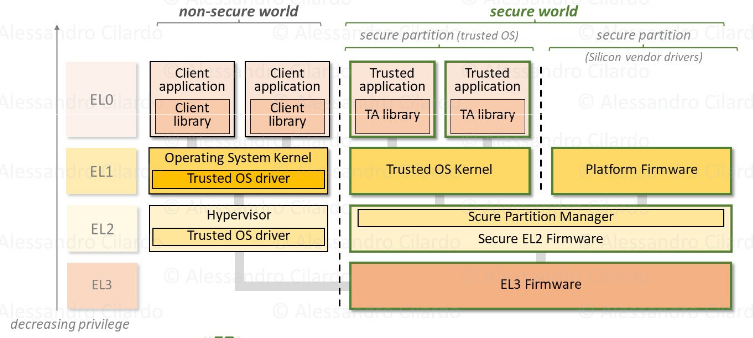
\includegraphics[width=.90\textwidth]{figures/ch3/virtualization/secure-virtualization.png}
  \end{center}
  \caption{Virtualizzazione sicura in ARMv8.4}\label{fig:secure-virtualization}
\end{figure}

Si hanno sempre $2$ livelli di traduzione. In \textbf{stage 1}, se si è in un \textit{non secure state}, allora gli indirizzi \textit{IPA} e \textit{PA} sono sempre \textit{non secure}: di fatto in questo caso si ha solo un tipo di indirizzo fisico. Invece, se si parte da un \textit{secure state}, allora l'uscita può essere sia \textit{secure} che \textit{non secure}. Quindi, si hanno $2$ possibili \textit{IPA (secure IPA e non secure IPA)} ciascuno dei quali conduce ad un \textit{secure PA e non secure PA} (\cref{fig:secure-address-translation})

\begin{figure}[H]
  \begin{center}
    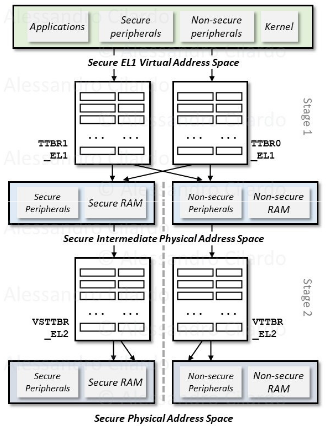
\includegraphics[width=.4\textwidth]{figures/ch3/virtualization/secure-address-translation.png}
  \end{center}
  \caption{Traduzione a due livelli di indirizzi partendo da \textit{secure state}}\label{fig:secure-address-translation}
\end{figure}


\subsubsection{Virtual Host Extentions - VHE}
In ARMv8, un hosted Hypervisor esegue in EL2 mentre l'host in EL1. Questo risulta inefficiente perchè il passaggio continuo tra EL1 (dove risiede la maggior parte del codice del sistema operativo host) e EL2 (dove risiede la maggior parte del codice relativo) è oneroso. A tal proposito a partire da ARMv8.1 sono state introdotte le \textbf{Virtualization Host Extensions (VHE)} che semplificano gli hypervisor permettendo una co-esistenza del sistema operativo host e dell'hypervisor in EL2 (\cref{fig:virtual-host-extensions}). Questa cosa risulta possibile impostando $HCR\_EL2.E2H=1$ (in modo da avere user/kernel space in EL2) e il bit $TGE$ che controlla quale spazio degli indirizzi virtuali è un utilizzo: 
\begin{itemize}
  \item $TGE=1$: sistema operativo host. In questa condizione tutte le eccezioni verranno inviate direttamente a EL2 dove si trova l'host OS;
  \item $TGE=0$: sistema operativo guest. Quando il kernel accederà ai registri EL1 verrà re-indirizzato a quelli giusti;
\end{itemize}

\begin{figure}
  \begin{center}
    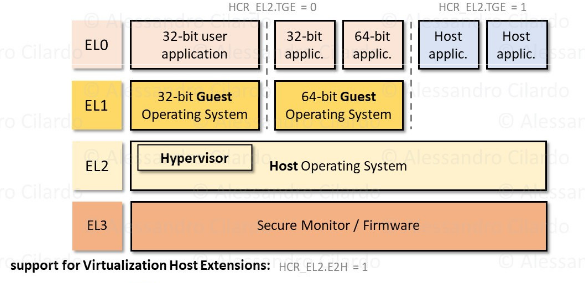
\includegraphics[width=.6\textwidth]{figures/ch3/virtualization/virtual-host-extensions.png}
  \end{center}
  \caption{Virtual host extensions}\label{fig:virtual-host-extensions}
\end{figure}

\clearpage
\subsection{Sicurezza}\label{sec:security}
\subsubsection{Introduzione}
Il focus principale di questa sezione è quello di fornire gli elementi fondamentali del \textbf{Confidential Computing}. L'acronimo CIA (\textbf{\textit{Confidentiality, Integrity, Availability}})indica le tre proprietà che un sistema deve garantire in ottica sicurezza. In particolare, il corso si focalizza su come garantire che il codice che viene eseguito a partire dalle prime fasi di avvio del sistema sia confidenziale (e quindi cifrato, non accessbile ad attori esterni) e integro (e quindi non manomesso). Inoltre, si introduce il concetto di \textbf{\textit{attestation}} in cuisi vuole verificare l'identità della piattaforma su cui si esegue un programma. Il modello di minaccia a cui si fa riferimento è quello in cui un attore malevolo potrebbe compromettere la \textbf{\textit{boot chain}} (installando un BIOS rootkit) o avere il controllo al livello sistema operativo attraverso dei moduli kernel (\cref{fig:system-overview}).

\begin{figure}[h]
  \begin{center}
    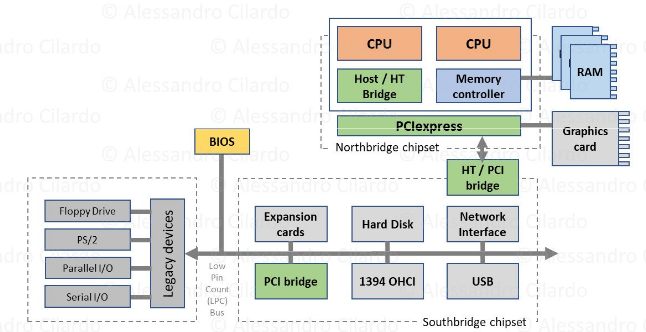
\includegraphics[width=.65\textwidth]{figures/ch3/security/desktop-pc-overview.png}
  \end{center}
  \caption{Overview di un sistema classico. Un potenziale attaccante potrebbe installare codice malevolo BIOS o in Hard Disk}\label{fig:system-overview}
\end{figure}

Il concetto principale dei sistemi di sicurezza è la \textbf{\textit{chain of trust}}. Sostanzialmente, consiste nella creazione di un sistema che calcola ricorsivamente l'hash dei componenti da caricare. Quindi, ogni componente ha una routine che calcola l'hash del successivo e lo verifica con un valore cablato. Ad esempio, il bootloader calcola l'\textit{hash} del sistema operativo e lo confronta con un valore cablato nell'immagine.
Un concetto chiave è quello di \textbf{chain of trust}. Il primo elemento di questa catena è detto \textbf{\textit{root of trust}}. Un altro concetto chiave è la \textbf{\textit{Trusting Computing Base} (TCB)}: l'insieme di componenti (hardware, software, infrastrutture o umani) di cui ci si può fidare.

\paragraph{Confidenzialità} Garantire la confidenzialità significa rendere non intelligibile i dati ad utenti non autorizzati. Questa proprietà viene garantita dalla crittografia cifrando le informazioni. In particolare, esistono due classi di algoritmi di crittografia: \textbf{a chiave asimmetrica} e \textbf{a chiave simmetrica}. La prima prevede l'utilizzo di due chiavi diverse per cifrare le informazioni: una pubblica e una privata (queste chiavi possono essere gestite a coppie o a gruppi) ed è alla base del meccanismo di firma digitale. La cifratura simmetrica prevede l'utilizzo della stessa chiave per la cifratura e decifratura e può risultare più semplice da implementare e meno robusto. Infatti, il problema principale degli algoritmi a chiave simmetrica è la condivisione delle chiavi. 

\paragraph{Integrità} Verificare l'integrità di un oggetto (hardware o software) significa certificare la sua provenienza. Tecnicamente, l'integrità viene controllata attraverso la tecnica dell'hashing è una tecnica utilizzata per trasformare un input di lunghezza arbitraria in un output di lunghezza fissa, chiamato valore di hash o digest. Gli algoritmi di hashing sono progettati per essere veloci e per produrre valori di hash unici per input diversi, minimizzando le collisioni (quando due input diversi producono lo stesso valore di hash). Gli algoritmi di hashing comuni includono MD5, SHA-1, e la famiglia SHA-2 (SHA-224, SHA-256, SHA-384, SHA-512). Una proprietà fondamentale degli algoritmi di hashing è che sono a senso unico, il che significa che è computazionalmente impraticabile risalire all'input originale a partire dal valore di hash.

\paragraph{Integrità} Verificare l'integrità di un oggetto (hardware o software) significa certificare la sua provenienza. Tecnicamente, l'integrità viene controllata attraverso la tecnica dell'hashing che si occupa di estrarre dall'oggetto che si vuole verificare un numero univoco. Le funzioni di \textit{hash} sono dette anche \textbf{\textit{one-way encryption}}: non consentono di ripristinare il contenuto. Esistono diversi algoritmi di hashing alcuni dei quali molto semplici e non con proprietà crittografiche (come \textbf{MD5}) mentre quelli più sicuri fanno parte della famiglia \textbf{\textit{Secure Hash Algorithms (SHA)}}. Il problema principale dell'hashing sono le \textbf{\textit{collisioni}}: in generale si desidera creare un'\textit{hash} univoco per ogni oggetto, ma questo non è possibile poichè bisogna rappresentare il risultato su una dimensione finita. Le funzioni di hashing sicuro aggiungono, oltre al contenuto, delle informazioni extra per ottenere anche a fronte dello stesso \textit{input}, \textit{output} diversi. Questo tipo di approccio funziona sulla base della \textbf{\textit{unforgiability}} dell'hash: non è possibile forzare un componente ad avere un'\textit{hash} che non sia il suo calcolato. Questa è una proprietà forte poichè non tutti gli algoritmi sono resistenti. Ad esempio, con \textit{MD5} è possibile modificare un input per avere un determinato \textit{hash} e quindi falsificare delle firme.

\subsubsection{Elementi di confidential computing}
Ci sono alcune definizioni di base del confidential computing che bisogna conoscere e sono elencate di seguito.

\paragraph{Integrità del sistema}
Con \textbf{Integrità} si indica il fatto che il sistema si comporta come previsto in fase di specifica. Dal punto di vista tecnico, al software viene associata un'identità che consiste in un \textit{hash}. Molti dei meccanismi di verifica sono basati sul controllo dell'hash.

\paragraph{Sealing}
Il sealing (\cref{fig:sealing}) è una tecnica duale a quella del binding in cui si vuole che l'accesso dipenda dalla configurazione del sistema. La cifratura (e la decifratura) includono una qualche informazione sull'identità specifica della piattaforma su cui ci si trova. Si può permettere la decifratura anche su una macchina fisica diversa che abbia però esattamente lo stesso firmware (bit per bit), lo stesso \textit{boot loader}. Un'applicazione che vuole fare sealing chiederà una chiave che dipende dallo stato del processore

\paragraph{Binding}
Con \textbf{\textit{binding}} (\cref{fig:binding}) si indica una cifratura portabile. L'accesso ai dati cifrati non dipende dalla configurazione del sistema, ma solo dalla chiave che a sua volta deve essere protetta. In questo caso, la chiave deve essere accessibile all'applicazione che la può utilizzare in maniera indipendente dalla piattaforma: i dati possono essere anche spostati durante il loro ciclo di vita.

\begin{figure}
\centering
\begin{subfigure}{.5\textwidth}
  \centering
  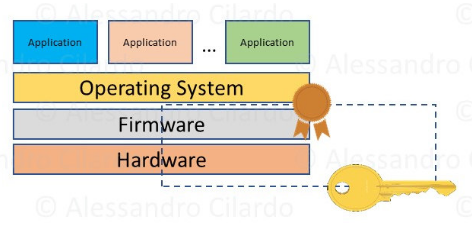
\includegraphics[width=.9\linewidth]{figures/ch3/security/sealing.png}
  \caption{Sealing}
  \label{fig:sealing}
\end{subfigure}%
\begin{subfigure}{.5\textwidth}
  \centering
  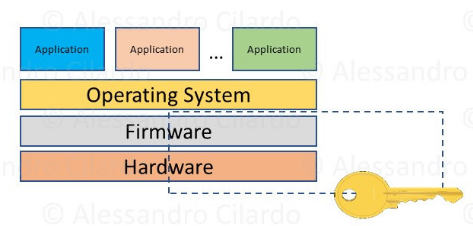
\includegraphics[width=.9\linewidth]{figures/ch3/security/binding.png}
  \caption{Binding}
  \label{fig:binding}
\end{subfigure}
\caption{Overview dei processi di sealing e binding}
\end{figure}

\paragraph{Process isolation}
Con questa tipologia si indica la separazione dello spazio di indirizzamento dei processi e può essere interpretata con diversi livelli di approfondimento. Ad esempio, potrebbe essere implementata semplicemente con una modalità utente e supervisore o con la virtualizzazione aggiungendo livelli come visto in \cref{sec:virtualization} creando molti strati di indirizzamento.

\paragraph{Remote attestation}
La \textbf{\textit{remote attestation}} offre la possibilità di verifica della piattaforma attraverso un entità di diverse parti. Ad esempio, un utente di un sistema cloud che esegue un'elaborazione su una macchina virtuale vuole avere la garanzia che la piattaforma hardware abbia degli standard di sicurezza prima di inviare i dati. Si instaura un canale, eventualmente cifrato, con una mutua autenticazione e si effettua un processo di \textit{challenge} con il quale si verifica l'identità della piattaforma e dello stack software fino ad un certo livello con un \textit{hash} firmato da un'entità fidata (molto similmente a quello che viene effettuato con \textit{https}). È possibile fare un'attestazione di \textbf{sciame} in cui si verifica un intero sistema fatto da più dispositivi.

La remote attestation è molto studiata anche nei sistemi IoT (per esempio anche sistemi in ambito industriale, droni) oggetti che sono dispiegati sul campo e che potrebbero essere modificati anche fisicamente da un attaccante. Esistono sono vari tipi di soluzioni anche tecnologiche, supportate chiaramente da un hardware che abbia qualche forma di \textit{tamper resistance} cioè che abbia un una chiave privata direttamente immessa nel silicio e un'area in cui vengono fatti i calcoli perl'attestazione all'interno di un perimetro sicuro. La \textit{tamper resistance} inibisce alcune modalità di attacco hardware che potrebbero solo essere attuate utilizzando tecniche e strumentazioni molto costose. Un altro concetto meno stringente è la \textbf{\textit{tamper evidence}}: consente di mettere fuori uso un dispositivo se questo viene manomesso.

\subsubsection{Tecniche di sicurezza hardware: Secure Boot, TPM e Disk Encryption}
Alcune tecniche di sicurezza base sono implementate anche all'interno dei normali PC. In questo caso, il threat model è più debole poichè non si vuole impattare tecnologie proprietarie. Con riferimento alla \cref{fig:system-overview}, vengono messi in sicurezza il BIOS, TPM e hard disk.
\begin{figure}[H]
\centering
\begin{subfigure}{.5\textwidth}
  \centering
  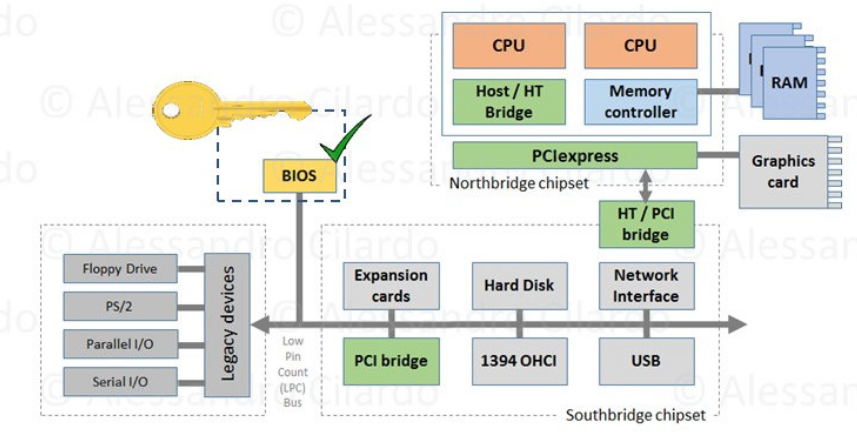
\includegraphics[width=.9\linewidth]{figures/ch3/security/secure-boot.png}
  \caption{Secure boot}
  \label{fig:secure-boot}
\end{subfigure}%
\begin{subfigure}{.5\textwidth}
  \centering
  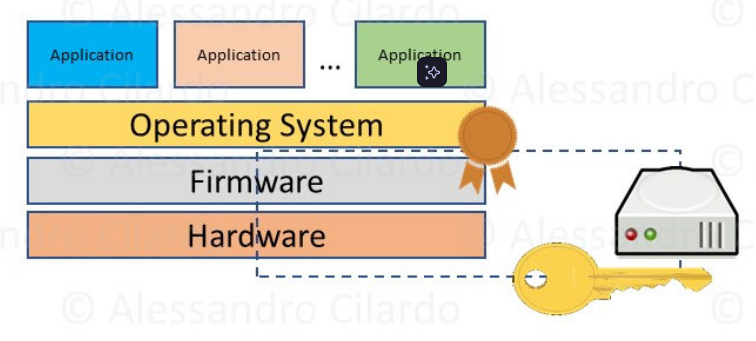
\includegraphics[width=.9\linewidth]{figures/ch3/security/disk-encryption.png}
  \caption{Disk Encryption}
  \label{fig:disk-encryption}
\end{subfigure}\\[1ex]
\begin{subfigure}{\linewidth}
  \centering
  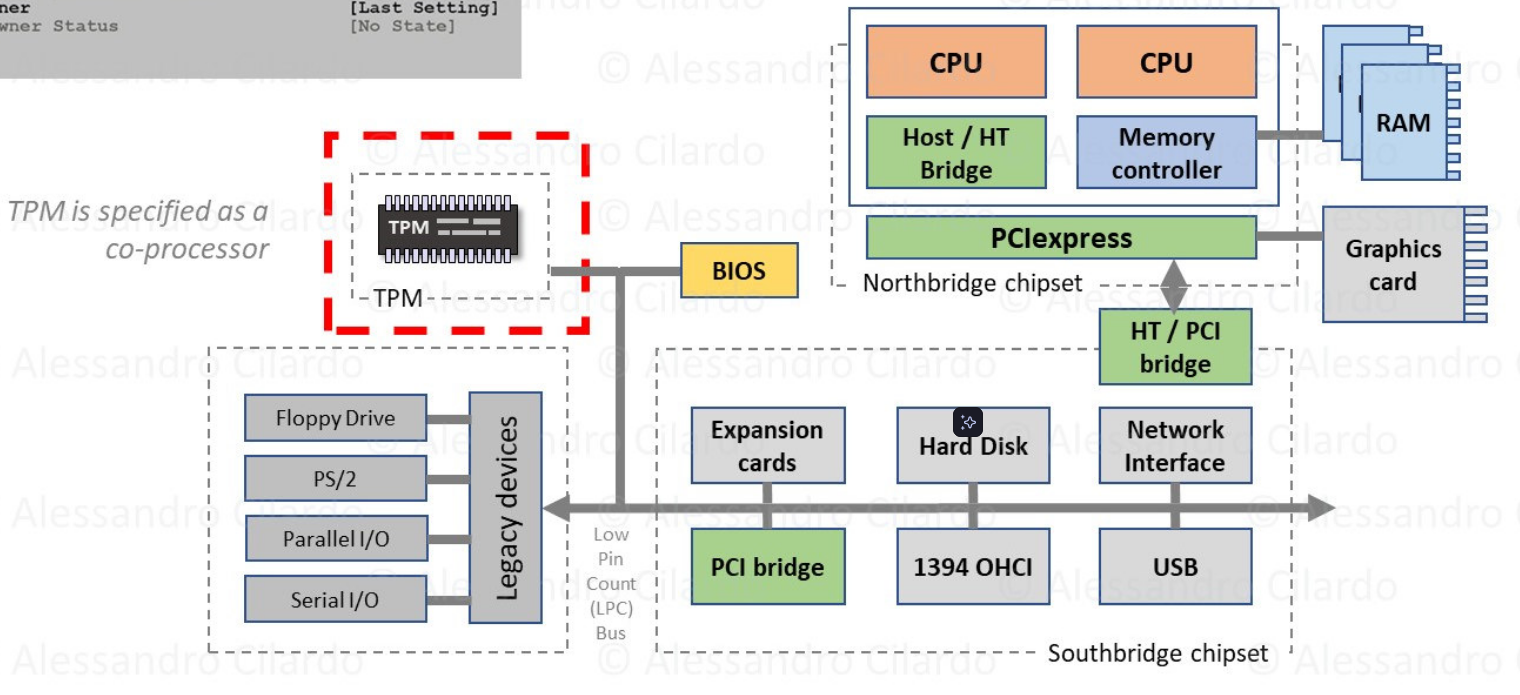
\includegraphics[width=.5\linewidth]{figures/ch3/security/tpm.png}
  \caption{TPM}
  \label{fig:tpm}
\end{subfigure}
\caption{Overview dei processi di sealing e binding}
\end{figure}
\paragraph{Secure boot}
Il \textbf{\textit{secure boot}} (\cref{fig:secure-boot}) verifica l'integrità del firmware che viene caricato all'avvio del sistema. Questo è esterno al processore e, pertanto, all'esterno del perimetro di sicurezza all'interno di una memoria non volatile che non ha nessuna protezione. Il \textit{secure boot} costruisece un perimetro di sicurezza attorno al firmware e prevede meccanismi di verificare l'integrità all'interno del processore.

\paragraph{Disk encryption}
Il \textbf{\textit{disk encryption}} (\cref{fig:disk-encryption}) è un meccanismo che protegge i dati mentre sono memorizzati. Esistono diverse soluzioni:
\begin{itemize}
  \item Linux Unified Key System (LUKS);
  \item BitLocker
\end{itemize}
La principale difficoltà di questa tecnologia è quella della gestione delle chiavi.

\paragraph{Trusted Platform Module: TPM}
Il TPM (\cref{fig:tpm}) è un oggetto che nasce come collaterale rispetto al processore: non era pensabile all’epoca di chiedere a AMD o Intel di modificare qualcosa che implicasse il processore stesso.  Il TPM è un modulo esterno simile ad una \textit{smart card} che supporta funzionalità crittografiche come firma verifica e hashing, ma non essendo integrato all'interno del processore può essere bypassato con modifiche hardware. Approfondendo il TPM in \cref{fig:tpm-detail}, si nota un parte di memoria in cui ci sono le chiavi e una di accelerazione in cui sono supportati diversi algoritmi. La parte più importante sono i $PCR_x$ (Platform Configuration Register) che contengono gli \textit{hash} al livello $x-esimo$ partendo da $0$ (livello firmware). Quest'architettura può essere utilizzata anche dalle macchine virtuali: è prevista la presenza di \textit{$0-virtuale$}. Come detto, nel modello di sicurezza non sono inclusi attacchi di tipo hardware: nessuno vieta di inserirsi tra processore e TPM e fingere delle risposte.

\begin{figure}[H]
  \begin{center}
    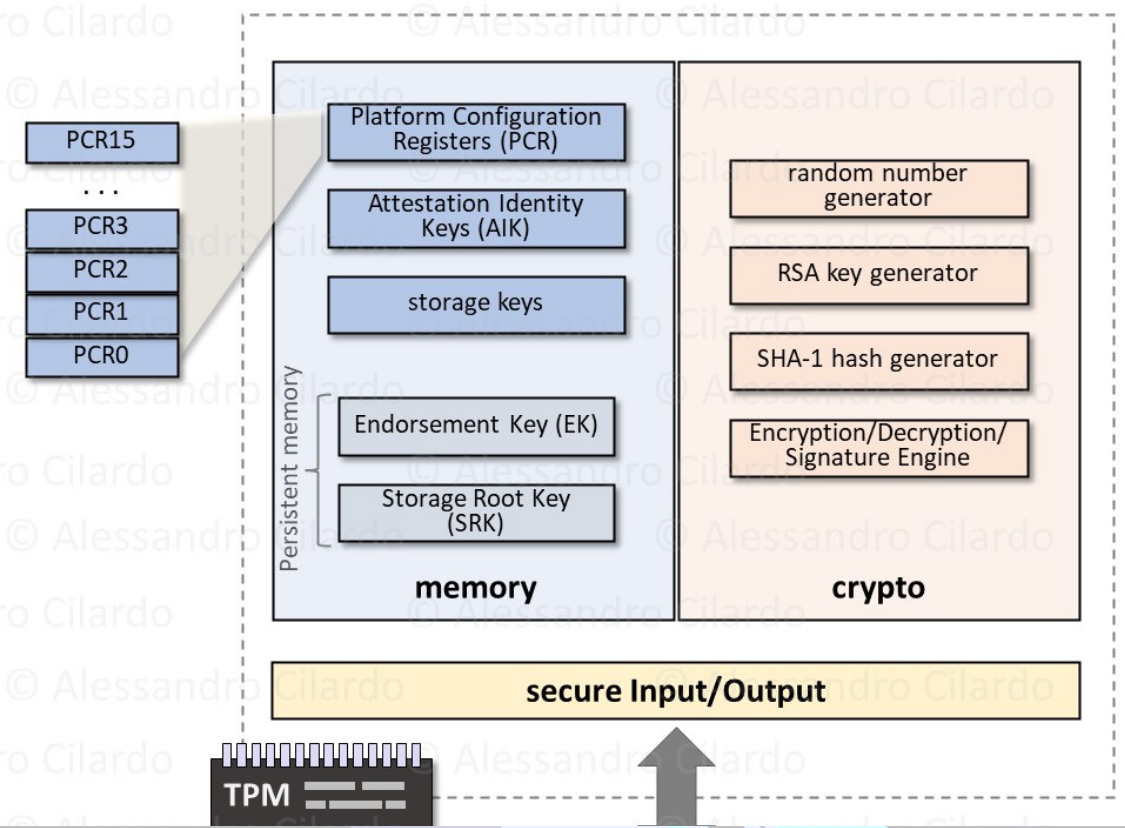
\includegraphics[width=.6\textwidth]{figures/ch3/security/tpm-detail.png}
  \end{center}
  \caption{Architettura interna del TPM}\label{fig:tpm-detail}
\end{figure}

Utilizzando il concetto di \textit{chain of trust}, il TPM è la \textit{root of trust}: se viene "violato" cade tutto il castello di carte. La TCB in questo caso è molto grande: bisogna fidarsi del produttore della CPU, della \textit{motherboard}, del \textit{manufacturer} (chi assembla il PC) ecc. Quindi non può essere utilizzata per applicazioni critiche.

Una delle cose che specifica TPM è una serie di criteri per costruire una gerarchia delle chiavi. Molto spesso le chiavi sono ottenute mediante un processo che si chiama \textbf{\textit{key derivation}} grazie al quale è possibile deterministicamente immaginare di ricostruirsi una chiave a partire dal possesso di una chiave sovrastante che spesso viene chiamata \textit{master key}. Ad esempio, un'azienda che installa tornelli deve fare in modo che ogni tornello abbia la propria chiave. Ciò avviene attraverso un modulo \textbf{\textit{SAM}} (quindi una specie di TPM o di SIM) che ha una master key comune a tutti ma che poi usa per derivare all’occorrenza una chiave specifica del dispositivo concatenando l’id del dispositivo (il serial number) con la master key e facendone un \textit{hash} una cifratura o comunque un qualcosa che dipende in maniera unidirezionale da questo input. Questo meccanismo di generazione è molto utile:

\begin{itemize}
  \item è possibile creare chiavi senza memorizzarle;
  \item è possibile cifrare file diversi con chiavi diverse aggiungendo nei metadati l'ID della chiave da utilizzare per cifrarla;
\end{itemize}

Le chiavi generate e memorizzate devono essere cifrate. Questo viene fatte con le \textit{storage key} (\cref{fig:tpk-key-hierarchy}). Per l'attestazione delle chiavi, il TPM ha un certificato pubblico firmato da un'autorità.
\begin{figure}[H]
  \begin{center}
    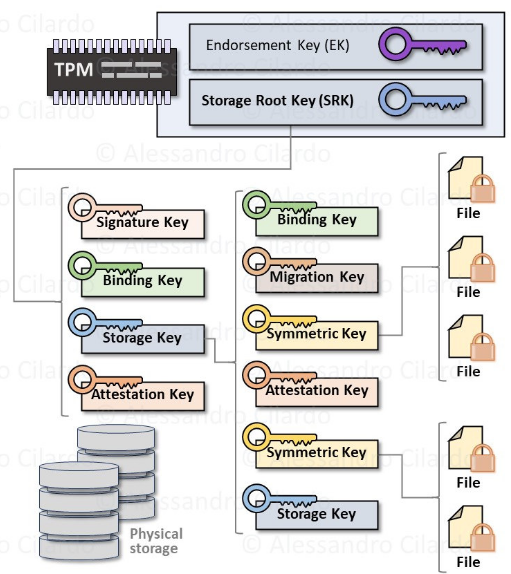
\includegraphics[width=.5\textwidth]{figures/ch3/security/tpm-key-hierarchy.png}
  \end{center}
  \caption{Gerarchia delle chiavi nel TPM}\label{fig:tpk-key-hierarchy}
\end{figure}

\subsubsection{Trusted computing al giorno d'oggi}
Tutti i concetti visti in precedenza, sono consolidati da molti anni. Tuttavia, a partire dal $2010$ ci si è iniziato a focalizzare su realizzare architetture che possano resistere ad attacchi hardware mirati cercando di realizzare applicazioni che possano ridurre la TCB includendo solo la CPU. In questo senso, si è introdotto il concetto di \textbf{\textit{Trusted Execution Enviornment}} (TEE) in cui si prevede a livello architetturale un'area di memoria dedicata ad un processo \textit{trusted} che non è accessibile agli altri dall'esterno. Ci sono diverse implementazioni del \textit{TEE}. Ad esempio, Intel con SGX introduce un'area di memoria separata detta \textbf{\textit{enclave}} cifrata. Quando il processore carica in cache le pagine, queste vengono decifrate. Al contrario, \textbf{\textit{Arm-TrustZone}} non prevede la parte di cifratura della memoria. In particolare, il concetto di ARM TrustZone è legato sia al Cortex-M che al Cortex-A, ma l'implementazione può essere profondamente diversa. Un micro-processore è molto più semplice di un application processor e, per differenziare, si usa il termine \textbf{\textit{Secure Process Enviornment (SPE)}}.

Questo concetto di separazione e isolamento è stato coniugato insieme alla virtualizzazione. Infatti, prima AMD propose \textbf{\textit{Secure Virtual Machine} (SVM)} con cui si utilizzza il TPM per controllare l'integrità del firmware prima di eseguire una macchina virtuale. A seguito dell'introduzione di TEE, AMD ha introdotto \textbf{\textit{Secure Encrypted Virtualization}}, orientato alla macchine virtuali, che, come Intel SGX, cifra la DRAM. Infine, sempre nel campo della virtualizzazione, Intel ha proposto \textbf{\textit{Trusted Domain eXtention} (TDX)}. Questa tecnologia deve avere un hypervisor che supporta questa estensione che fondamentalmente divide lo spazio in \textbf{\textit{trusted}} e \textbf{\textit{untrusted}}.

\paragraph{Remote Attestation} L'\textbf{\textit{attestation}} è un processo che serve a verificare l'autenticità di una piattaforma sulla quale si sta per effettuare un'elaborazione. In pratica, si crea una firma che attesta l'identità di un processore. Intel ha introdotto il processo di attestazione remota in cui mette a disposizione un servizio per verificare l'autenticità dei \textit{report} generati. Esistono diversi modi di realizzare questa funzionalità. Ad esempio, Intel ha implementato con il nome EPID, il protocollo \textbf{\textit{Direct Anonymous Attestation (DAA)}}: un gruppo di dispositivi, ciascuno con la propria chiave privata, può firmare un oggetto che può essere verificata con una chiave di gruppo.

\paragraph{ARM TrustZone} TrustZone è un meccanismo architetturale per la creazione di TEE che nasce in ARMv6. Nelle prime versioni (\cref{fig:armv6-trustzone}), era abbastanza rudimentale e permetteva solo di aggiungere un bit a tutte le transazioni (verso la memoria, dispositivi ecc) marcandole come \textbf{\textit{secure}} o \textbf{\textit{normal}}. Questa divisione è ortogonale alla divisione utente/supervisore: codice \textit{secure} può essere utilizzato sia in maniera privilegiata che non. Il bit $NS$ corrisponde ad un collegamento fisico che può decidere il comportamento di altri componenti come TrustZone Memory Adapter (TXMA), TrustZone Address Space Controller (TZASC, partiziona lo spazio di memoria in maniera particolare), TZ-DMA (controller che possono controllare l'accesso alla memoria di periferiche non sicure). Inoltre, ARM specifica una particolare istruzione \textbf{\textit{Secure Monitor Call (smc)}} che consente di effettuare un \textit{context switch} di sicurezza per passare da una modalità all'altra (\cref{fig:arm-trustzone-implementation}).

In ARMv6, non c'era una strutturazione precisa della TCB e mancava un meccanismo di boot sicuro; con ARMv7 e ARMv8-A/M è stata aggiunta la possibilità di avere trusted \textit{firmware} e la possibilità di avere una TCB ben definita con una \textit{root of trust}. Global Platform definisce un insieme di API standard per dialogare con le TEE. Infine, ARM ha lanciato \textbf{\textit{Platform Security Architecture (PSA)}} per dare delle linee guida da seguire per sviluppare codice sicuro fornendo esempi con trusted firmware.

\begin{figure}
  \begin{center}
    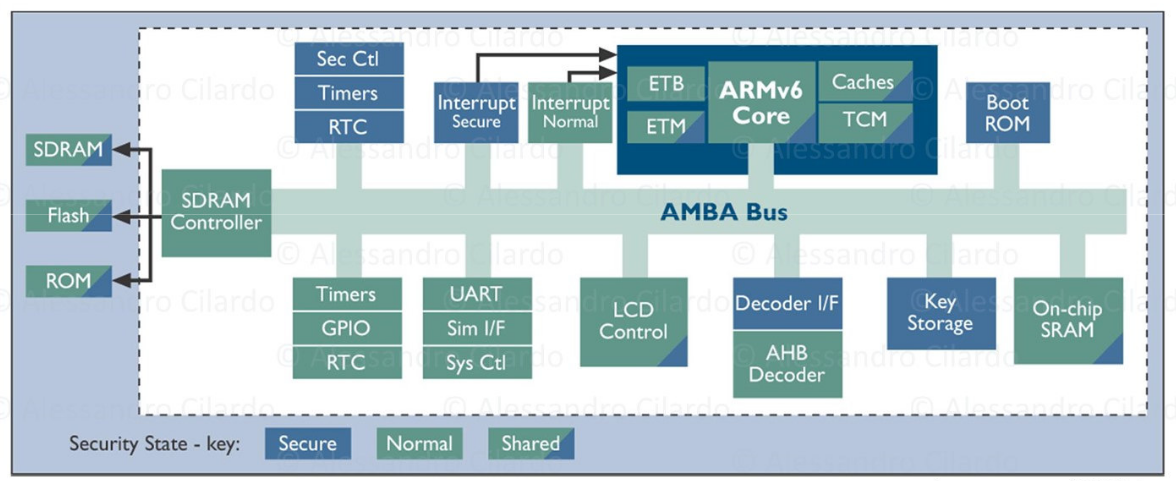
\includegraphics[width=.75\textwidth]{figures/ch3/security/armv6-trustzone.png}
  \end{center}
  \caption{Architettura ARMv6-TrustZone}\label{fig:armv6-trustzone}
\end{figure}

\begin{figure}[H]
  \begin{center}
    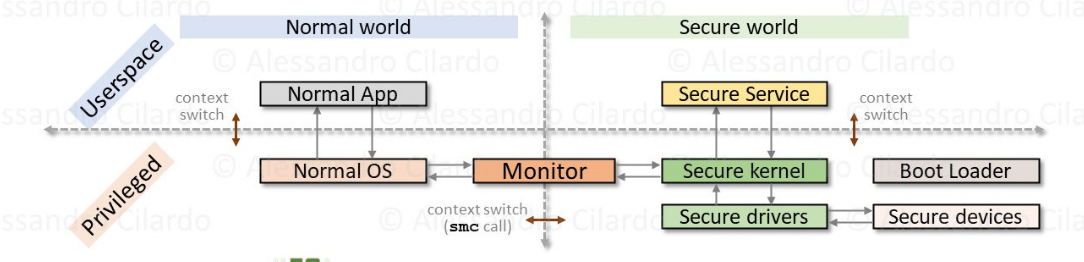
\includegraphics[width=.85\textwidth]{figures/ch3/security/arm-trustzone-implementation.png}
  \end{center}
  \caption{Overview del passaggio da secure world a normal world}\label{fig:arm-trustzone-implementation}
\end{figure}

Con riferimento ad ARMv8, un sistema sicuro che utilizza trustzone è mostrato in \cref{fig:armv8-trustzone-state}. La strutturazione in livelli di privilegio ha nell’ EL3 quello più “potente”, il quale è usato soltanto per il secure monitor, che fa le veci del secure word di Trust Zone. In particolare, lo scenario mostrato è quello nel quale EL3 gira a 64 bit (i livelli successivi sono sia a 32 che a 64): questo consente di essere compatibili con una certa architettura della memoria virtuale (VMSAv7), la quale è a 32 bit ed è diversa dall’architettura a 64 bit. La parte di secure OS ci consente di far girare applicazioni in modalità sicura: il kernel di un secure OS deve essere piccolo perché spesso questi software sono oggetto di verifica che esplode in complessità se si mette un software complesso.

\begin{figure}
  \begin{center}
    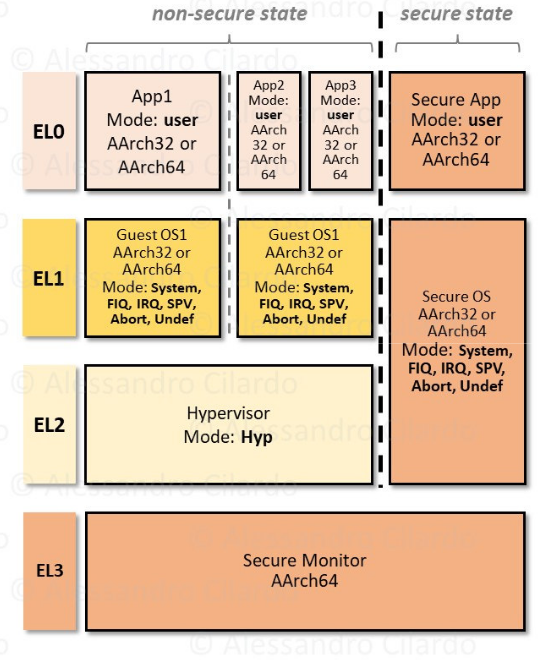
\includegraphics[width=.5\textwidth]{figures/ch3/security/armv8-trustzone-state.png}
  \end{center}
  \caption{Gestione di secure state e non secure state in ARMv8}\label{fig:armv8-trustzone-state}
\end{figure}

\subsubsection{Platform Level Security: Zynq Ultrascale+}
In questa sezione sono elencati quali sono i problemi che un ente che integra ARM sulla sicurezza. Il focus è sulla Zynq-Ultrascale+ che utilizza un FPGA Xilinx: tutti i meccanismi illustrati sono proprietari di Xilinx e non generalizzabili.

I concetti di TrustZone devono essere implmentati ed estesi in MPSoC dal manufacturer. Infatti, la parte di sicurezza deve includere anche periferiche ed interconnessioni che esulano da ARM: si parla di \textbf{\textit{platform level security}}. Nella Zynq-Ultrascale è presente un ARMv8-A con un FPGA che può accedere al bit $NS$ di ARM per configurare eventualmente periferiche in modo sicuro. Dal punto di vista della sicurezza, deve essere gestito perchè l'FPGA si configura dall'esterno e, pertanto, può essere esposto. In particolare, la Zynq mette a disposizione meccanismi per combinare \textbf{\textit{secure boot}} e cifratura del \textit{bistream}. Prendendo l'FPGA, il bitstream è cifrabile con una chiave AES direttamente da Vivado: questa chiave è possibile bruciarla una sola volta nel circuito o metterla in una RAM con alimentazione dedicata. Inoltre, è possibile autenticare il \textit{bitstream} conservando un \textit{hash} della chiave pubblica.

Con riferimento alla \cref{fig:zynq-ultrascale-arch}, si nota che il processore non è l'unico attore attivo nel sistema, ma altri componenti possono agire da \textit{master} nel sistema facendo partire le transazioni di lettura e scrittura. Questo potrebbe rapppresentare un problema di sicurezza e Xilinx ha creato dei blocchi aggiuntiv di interconnessione configurabili via software:

\begin{itemize}
  \item \textbf{\textit{XMPU}}: sono simili agli MPU, hanno degli intervalli configurabili, a ciascuno di questi è associata una maschera che identifica uno o più ID di master che sono presenti nel sistema. Applica dei controlli sulla combinazione di master che fa la richiesta e intervalli di memoria. Sono configurabili (in maniera trusted) tramite dei registri che permettono di cambiare questo tipo di scelta. Se avvenisse una violazione, si può decidere di innescare un fault o gestire l’operazione in maniera apparentemente normale. Ad esempio, si può reindirizzare l’operazione verso una sorta di periferica sink per la logica di gestione;
  \item \textbf{\textit{XPPU}}:  è molto simile alla \textit{XMPU}, ma è dedicata alle periferiche. Non ha nozione degli internalli di memoria e consente di controllare gli indirizzi degli \textit{slave};
\end{itemize}

Sempre con riferimento all'architettura è possibile notare differenti domini di potenza nell'MPSoC: regioni fisiche alimentate in maniera separata dalle altre. Ad esempio, la regione \textbf{\textit{low power}} rappresenta la parte sempre accesa del dispositivo, mentre quella \textbf{\textit{full power}} è pensata per i componenti che consumano di più.

\begin{figure}[H]
  \begin{center}
    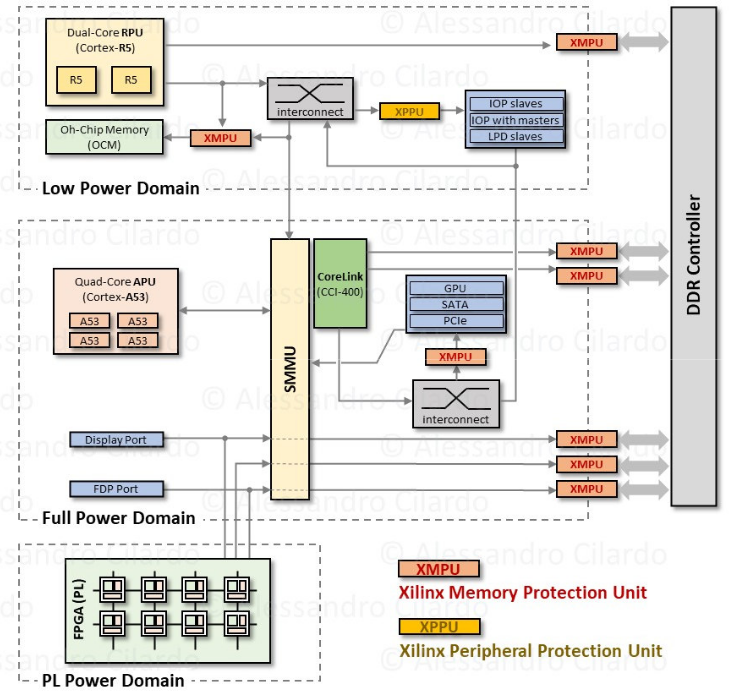
\includegraphics[width=.75\textwidth]{figures/ch3/security/zynq-ultrascale-arch.png}
  \end{center}
  \caption{Schema a blocchi della Zynq-Ultrascale}\label{fig:zynq-ultrascale-arch}
\end{figure}

Un componente fondamentale è la \textbf{\textit{Configuration Secure Unit}(CSU)} ed è divisa in due parti (\cref{fig:zynq-ultrascale-csu}):
\begin{itemize}
  \item \textbf{\textit{Secure Processor Block (SPB)}};
  \item \textbf{\textit{Crypto Interface Block (CIB)}};
\end{itemize}

Il \textit{CIB} offre funzionalità di accelerazione crittografica. Ci sono degli acceleratori che possono eseguire RSA, SHA3, AES e possono essere usati sia da FPGA (per operazioni sul \textit{bistream}), \textit{First Stage Boot Loader (FSBL)} e applicazioni utente. Un altro elemento del \textit{CIB} è il \textbf{\textit{Processor Configuration Access Port (PCAP)}}: una periferica che permette di configurare l'FPGA da \textit{software} consentendo di modificare il suo comportamento dinamcamente. Questo è utile per effettuare diversi tipi di inferenza facendo \textbf{\textit{ensamble learning}}.

\begin{figure}[H]
  \begin{center}
    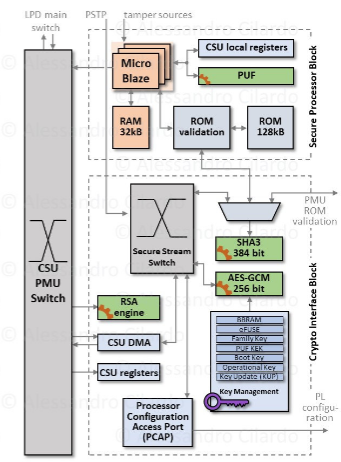
\includegraphics[width=.5\textwidth]{figures/ch3/security/zynq-ultrascale-csu.png}
  \end{center}
  \caption{Configuration Secure Unit nella Zynq-Ultrascale}\label{fig:zynq-ultrascale-csu}
\end{figure}

L'\textit{SPB} rappresenta la parte blindata della CSU e contiene la \textit{ROM} che rappresent la \textit{root of trust}, poiché ci sono le prime che istruzioni che vengono caricate che poi a loro volta si incaricano di capire dove sta il \textit{boot loader}. Questo codice è chiuso, nel senso è già scritto da Xilinx e viene anche validato con un calcolo dell’hash. Questo codice di root non viene eseguito su ARM, ma su un processore \textbf{\textit{Micro Blaze}} all’interno di SPB in configurazione \textit{TMR}. Un altro pezzo degno di nota è il \textbf{\textit{Physically Unclonable Function (PUF)}} (\cref{fig:puf-structure}): un blocco HW che può essere implementato in diversi modi. Uno di questi è quello di mettere in corto circuito una catena di buffer per causare un’oscillazione. Questa oscillazione è non è aleatoria ma dipende dal ritardo che si ha lungo la catena di \textit{buffer}. Poichè a livello microscopico è impossibile creare due circuiti identici, la \textit{PUF} può creare un'impronta digitale del chip non controllabile dall'azienda manufatturiera. Inoltre, non sempre è implementata e in tal caso può essere sostituita da un valore pubblico non modificabile detto \textbf{\textit{DNA}}.

\begin{figure}
  \begin{center}
    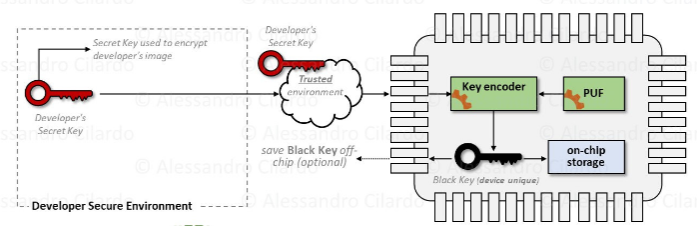
\includegraphics[width=.7\textwidth]{figures/ch3/security/puf-structure.png}
  \end{center}
  \caption{PUF}\label{fig:puf-structure}
\end{figure}

\paragraph{Key management}
Il PUF, può essere molto utile nel momento in cui bisogna generare una chiave di cifratura per il \textit{bitstream} e per il \textit{FSBL}. Il problema di \textbf{\textit{key management}} non è un problema tecnologico, ma di \textit{policy}. Infatti, bisogna trovare un \textbf{\textit{trade-off}} tra praticità e sicurezza. Un elemento aggiuntivo è la possibilità di mettere una chiave che è unica, controllata da Xilinx (nota solo all'azienda) e comune a tutti i dispositivi di una certa famiglia detta \textbf{\textit{Family Key}}. Questa chiave non è molto utile dato che è comune a gruppi di dispositivi, ma può essere utilizzate perchè in alcune situazioni non è possibile generare una chiave sicura e questa chiave potrebbe essere utile per cifrare la chiave privata con la \textit{Family Key} fidandosi di Xilinx. Nel boot, ci sarà la chiave che sarà cifrata tramite la family key classica e la chiave decifrata sarà utilizzata per l'FPGA.

\paragraph{Key rolling} Anche gli algoritmi più efficaci ppssono soffrire di attacchi hardware detti \textbf{\textit{side channel attacks}} in cui il "canale" è qualsiasi fenomeno fisico misurabile dall'esterno che possa dare informazioni sul valore della chiave. Ad esempio, la misura del tempo di esecuzione, di potenza può dare informazioni sul particolare path attivato nel momento in cui la chiave viene utilizzato (ad esempio le operaizioni di AND con uno zero possono essere più rapide). Per mitigare questi attacchi, bisogna utilizzare una chiave il meno possibile su meno dati possibile. 

Ad esempio, l'algoritmo AES lavora su $256 bit$. Il \textbf{\textit{key rolling}} (\cref{fig:key-rolling}) divide i dati in mini-blocchi che vengono decifrati in sequenza. Una parte del blocco decifrato include la chiave per decifrare il prossimo in modo tale da avere chiavi diversi utilizzate per una minor quantità di dati.

\begin{figure}[H]
  \begin{center}
    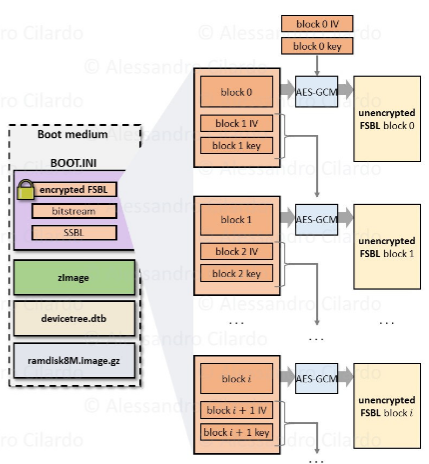
\includegraphics[width=.5\textwidth]{figures/ch3/security/key-rolling.png}
  \end{center}
  \caption{Overview key rolling}\label{fig:key-rolling}
\end{figure}

\paragraph{Anti-tampering}
Ci sono altri meccanismi che sono pensati per rispondere a dei requisiti di certificabilità in terminidi sicurezza, basati su vari standard, i quali definiscono dei requisiti per delle crypto engine. Ad esempio, i requisiti possono specificare di reagire in maniera attiva agli attacchi (ad esempio effettuando uno zero-ing della memoria) o misure passivi (come disabilitare porto di debug). Rilevare gli attacchi è un'attività complicata e richiede hardware apposito. Un attaccante potrebbe indurre selettivamente dei fault e cercare di ricavare informazioni su cosa effettivamente sta facendo il dispositivo. 

\end{document}
